% !TeX spellcheck = en_GB
\documentclass{template}

\usepackage{makros}



% metadata
\titlehead{
\includegraphics[height=1.4cm]{rwth.pdf} \hspace{1cm}

\includegraphics[height=1.4cm]{IGPM_logo_klein.png}
}

\subject{Master Thesis}
\title{Discontinuous Galerkin Methods for the \MA Equation}
\subtitle{\Large Discontinuous Galerkin Verfahren zur Lösung der Monge-Amp\`ere-Gleichung}
\author{Elisa Friebel} %\\ Matrikelnummer: 295932
\date{\today}
\publishers{Gutachter: Prof. Dr. rer. nat. W. Dahmen\\ Prof. Dr. rer. nat. S. Noelle}

% begin document
\begin{document}


\pagenumbering{Alph}
% title page
\maketitle
%\cleardoublepage

% erklärung
\begin{center}
\begin{minipage}[t]{0.8\textwidth}

\chapter*{Erklärung}
Ich versichere hiermit, dass ich die vorliegende Arbeit selbständig und
ohne Benutzung anderer als der angegebenen Hilfsmittel angefertigt habe.
Alle Stellen, die wörtlich oder sinngemäß aus veröffentlichten und nicht
veröffentlichten Schriften entnommen sind, sind als solche kenntlich
gemacht.

\vspace{1cm}
Aachen, den \today

\vspace{2cm}
(Elisa Friebel)
\end{minipage}
\end{center}
\thispagestyle{empty}
\cleardoublepage

% toc
\pagenumbering{roman}
\tableofcontents{}

%\cleardoublepage
\setcounter{page}{1}
\pagenumbering{arabic}

% content

% warum wollen wir etwas tun?was wollen wir tun? welche kapitel gibt es?
%\chapter*{Preface}
%\label{ch:preface}
%\ input{preface.tex}

% wie sieht das mathematische modell aus?
\chapter{Mathematical foundations}
\label{ch:TheoreticalBackground}
\section{ Preliminaries and Notation}
At the beginning of this chapter we repeat the basic definitions and notation for the analysis of partial differential equations as they are introduced for example in \cite[Introduction]{Evans1998}.
Let $\Omega \subset \R^d $ be an open, bounded area and $\partial \Omega$ its boundary.
\begin{definition}[Partial Differential Equation{\cite[Introduction]{Evans1998}}]
 A \emph{partial differential equation} (PDE) of order $k\in \N$ is an expression of the form
\begin{align}
	F(D^k u(x), D^{k-1}u(x), \dots, Du(x), u(x), x) = 0, (x \in \Omega)\label{eq:general PDE}
\end{align}
where $F:\R^{n^k} \times \R^{n^{k-1}} \times \dots \times \R^n \times \R \times \Omega \rightarrow \R $ is given and $u:\Omega \rightarrow \R$ is unknown.
\end{definition}
We focus in this thesis on second-order PDEs for our main PDE, namely the \emph{\MA equation} which we will introduce later is of second order. 
\\Next to the order there exist further properties to categorise PDEs:
\begin{definition}[Categories of PDEs{\cite[Introduction]{Evans1998}}]
	Given functions  $f:\Omega \rightarrow \R$ and $a_{\alpha}:\Omega \rightarrow \R$ or $a_{\alpha}:\R^{n^{k-1}} \times \dots \times \R^n \times \R \times \Omega$ respectively, for $\alpha \in \N^{k}, |\alpha| \leq k$, a PDE of order $k$ is called
	\begin{enumerate}[(i)]
		\item \emph{linear} if it can be written in the form
		\[
			\sum_{|\alpha| \leq k} a_{\alpha} (x) D^{\alpha} u(x) = f(x).
		\] 
		
%		\item \emph{semilinear} if it can be written in the form
%		\[
%			\sum_{|\alpha| = k} a_{\alpha}(x) D^{\alpha} u + a_0(D^{k-1}u, \dots, Du, u, x)= f(x),
%		\]	
%		i.e. a semilinear PDE is nonlinear in the unknown function, but linear in all partial derivatives.
		
		\item \emph{quasilinear} if it can be written in the form
		\[
			\sum_{|\alpha| = k} a_{\alpha}(D^{k-1}u, \dots, Du, u, x) D^{\alpha} u + a_0(D^{k-1}u, Du, u, x)= f(x),
		\]	
		i.e. a quasilinear PDE is nonlinear in (at least) on lower derivate, but linear in the highest order derivates.
		
		\item \emph{fully nonlinear} if it depends nonlinearly upon the highest order derivatives.
	\end{enumerate}
\end{definition}
A famous example for linear PDEs is the \emph{Poisson equation} $-\triangle u = f$,
% a semilinear PDE is for example the \emph{nonlinear Poisson equation} $-\triangle u = f(u)$.
a well-known example for quasilinear PDEs are equations of the type $\nabla \cdot (A(u) \nabla u) = f$, where $A: \R^d \rightarrow \R^{d \times d}  $. The \MA equation $\mydet {D^2 u} = f$ is part of the last category, the nonlinear PDEs. 

Another important property to classify second-order PDEs is ellipticity. 
\begin{definition}[Elliptic PDE{, \cite[p.207]{FGN2013}}]
	A fully nonlinear second order PDE is called \emph{elliptic} if its operator satisfy
	\begin{align}
		F(A,p,z,x) \leq F(B,p,z,x) \label{eq: ellipitic PDE}
	\end{align}
for all $x \in \Omega, z \in \R, p \in \R^d$ and $A,B \in \R^{d \times d}_{sym}$  with $A-B$ positive definite.

This notion is a natural extension of the ellipticity concept for first order PDEs. Interpreting a first order PDE operator as a Function depending on $D^2u, Du, u, x$, \eqref{eq: ellipitic PDE} characterises an elliptic PDE.
\end{definition}

Searching for a function $u:\Omega \rightarrow \R$ with 
\begin{align}
u=g \text{ on } \partial \Omega \label{eq: boundary}
\end{align}
for some $g:\partial \Omega \rightarrow \R$ is called a \emph{Dirichlet-boundary problem}. The function $u:\Omega \rightarrow \R$ fulfilling \eqref{eq:general PDE} and \eqref{eq: boundary} is called a classical solution of the problem. 
\todo{boundary conditions}

There are problems such that no such solution exists. A PDE of order $k$ requires its classical solution to be at least $k$ times differentiable, which is a very strong demand. To admit less regular solutions one aims for a weaker notion of a solution. Before doing this we specify some function spaces.

%\section{Functional Spaces}
According to the literature we refer by $W^{s,p}(\Omega)$ to the H\"older space, a set consisting of all $L^p(\Omega)$ functions whose distributional derivates up to order $s$ are contained in $L^ p(\Omega)$.
\todo{Sollte ich  distributional derivates erklaeren?} The special case $p=2$ are referred to as Sobolev spaces $H^s(\Omega):=W^{s,2}(\Omega)$. An additional subscript $0$ denotes the set where all functions are zero at the boundary, i.e. $H^s_0 :=\{f \in H^s(\Omega); f(x)=0 \; \forall x \in \partial \Omega\}$

Let $T$ be a triangle in $\Omega$ and spanned by the points $v_0, v_1, v_2$. We also write 
\[
	T= \langle v_0, v_1, v_2 \rangle := \{\beta_0 v_0+ \beta_1 v_1 +\beta2 v_2; 0 \leq \beta_i \leq 1, i= 0,1,2\}.
\]
The \emph{diameter} $diam(T)$ of a triangle $T$ we define as the diameter of the smallest circle containing it.
To discretise our domain $\Omega$ we subdivide it into simplices, more precisely we divide them into triangles.
\begin{definition}[Triangulation, {\cite[Definition 5.1]{Braess2003}}]
	We call a finite partition of $\Omega$ into triangles $\{T_1, \dots, T_n\}$ a feasible \emph{triangulation} $\mathcal{T}$, such that
	\begin{enumerate}[(i)]
		\item	$\bar \Omega = \bigcup_{T \in \triang} T_i$
		\item If $T_i \cap T_j$ is a point for, it is a vertex of both $T_i$ and $T_j$
		\item If $T_i \cap T_j$ is more than one point for $i \neq j$, it is an edge of both $T_i$ and $T_j$
	\end{enumerate}
	Let $h$ denote the maximal diameter $h:= \operatorname{max}\limits_{T\in \mathcal T} diam(T)$ in the triangulation $\mathcal T$, we then also refer to $\mathcal{T}$ by $\triang$. We call a triangulation \emph{regular} if every element is congruent.
\end{definition}
Note that this definition requires $\Omega$ to be a polygonal domain. However, there are extension to domain with curved boundaries: In those triangles lying at the boundary are replaced by "triangles" which have curved sides. 

\begin{figure}[H]
\usetikzlibrary{calc}

		\begin{center}
		\begin{tikzpicture}[scale = 5]
%define coordinates
			\coordinate (vEins) at (0,0) ;
			\coordinate (vZwei) at (0:4cm);
			\coordinate (vDrei) at (90:4cm);

%draw square
			\draw (0,0) -- (1,0) -- (1,1) -- (0,1) -- cycle; 

%draw diagonals
			\draw (0,0) -- (1,1);
			\draw (1,0) -- (0,1);

			\draw (0.5,0) -- (1,0.5) -- (0.5,1)-- (0,0.5) --cycle; 

			\draw(0.25,0.25) -- (0.75,0.25) -- (0.75,0.75)-- (0.25,0.75) --cycle; 

			\draw node at (0.15,0.5) {$T_0$};

			\draw[color=blue, thick] (0.25,0.25)-- node[above]{\blue{$e_0$}} (0,0.5);
			\coordinate (vMiddle) ($(0.25,0.25)!0.5!(0,0.5)$);
			
			\draw[color=blue, thick, ->] ($(0.25,0.25)!0.5!(0,0.5)$) -- node[right=0.3, below=0.1]{\blue{$\mathbf n_{e_0}^{ T_0}$}} ($ ($(0.25,0.25)!0.5!(0,0.5)$) - (0.075,0.075)$);

		\end{tikzpicture}
		\end{center}

\caption{A regular triangulation of the unitsquare}
 \label{fig: triangulation}
\end{figure}

Figure \ref{fig: triangulation} shows a triangulation of the unitsquare. Since the edges uniquely define a triangulation of $\Omega$, we later use the terms grid and mesh to refer to a subdivision into triangles.
An edge $e$ is called an interior edge if $e=T^+ \cap T^-$ holds for some $T^+,T^- \in \triang$, whereas it is called a boundary edge if $e \subset \partial \Omega$.
We divide the edges $\edges$ into the subsets $\edgesi$ and $\edgesb$ containing all interior edges and boundary edges, respectively. 
When we refer to a normal of an edge we always refer to an outward directed normal of one of the adjacent triangles. If it is not clear from the context a superscript denotes which triangle we chose.

On this basis we define the piecewise spaces
\begin{definition}[Broken Spaces]
We define some function spaces associated to a triangulation
\begin{align}
	H^s(\triang) = \prod\limits_{T\in \triang}  H^s(T), \qquad W^{s,p}(\Omega) = \prod\limits_{T\in \triang} W^{s,p}(T).
\end{align}	

\end{definition}
\begin{definition}[Piecewise Polynomial Spaces] \label{def: piecewise polySpace}
	Further we denote the finite-dimensional space of piecewise polynomials by
\[	
	\mathcal P^k_h = \{ f \in L^\infty(\Omega); f \arrowvert_T \textnormal{ is a polynomial of (total) degree } \leq k \textnormal{ for every } t \in \mathcal T_h\}.
\]
\end{definition}

%\todo{norms}
We use a subscript $h$ to indicate a piecewise evaluation/interpretation. Subsequently differential operators with a subscript $h$ imply separate differentiations on every triangle.

To formulate a method capable of handling discontinuities along triangle edges we introduce edge operators.   

\begin{definition}[Edge Operators]
We denote the \emph{normal jump} of  a piecewise smooth function $u_h:\Omega \rightarrow \R$ across an edge $e \in \edges$ by
\begin{align*}
	\jump {u_h}&:= 
	\begin{cases}
		u_h^+  \mathbf n^+ + u_h^- \mathbf n^-  &\text{ if } \partial T^+ \cap \partial T^- = e \text{ for some }T^+,T^- \in \triang, \\
		u_h \mathbf n 	 &\text{ if } \partial T \cap \partial \Omega = e \text{ for } T \in \triang,
	\end{cases}	
\end{align*}
where $n^\pm$ are the normals with respect to $T^\pm$ and  $u_h^\pm(x) = \lim_{\varepsilon \rightarrow 0} u_h(x-n^\pm \varepsilon)$.
Likewise we define the normal jump of a piecewise smooth function $u_h:\Omega \rightarrow \R^2$ across an edge $e \in \edges$ by
\begin{align*}
	\jump {u_h}&:= 
	\begin{cases}
		u_h^+ \cdot \mathbf n^+ + u_h^-\cdot  \mathbf n^-  &\text{ if } \partial T^+ \cap \partial T^- = e \text{ for some }T^+,T^- \in \triang,\\
		u_h\cdot \mathbf n 	 &\text{ if } \partial T \cap \partial \Omega = e \text{ for }T\in \triang.
	\end{cases}	
\end{align*}
Here $\cdot$ denotes the scalar product.
Note, that the jump of a scalar is a vector, whereas the jump of a vector is a scalar.

The \emph{average} of a piecewise smooth function $u_h:\Omega \rightarrow X$ for every $X$ across an edge $e \in \edges$ is defined by
\begin{align*}
	\average {u_h} &:= 
	\begin{cases}
	\frac 1 2 \left(u_h^+ + u_h^-\right) &\text{ if } \partial T^+ \cap \partial T^- = e \text{ for some }T^+,T^- \in \triang, \\
	 u_h &\text{ if } \partial T \cap \partial \Omega = e \text{ for }T\in \triang.
	\end{cases}
\end{align*}
\end{definition}


\section{Finite Element Method}
Before we discuss numerical schemes for the \MA equation we really shortly recall how a finite element method works, for a deeper insight in finite element methods we recommend \cite{Braess2003, BS2002}. Since the finite element method bases on a variational formulation we talk about finite element methods by the example of the general Poisson equation. 

%\subsection{The Poisson Problem}

\begin{definition}[Generalised Poisson Problem]
The \emph{Generalised Poisson Problem} is finding a function $u:\Omega \rightarrow \R$ such that 
\begin{align}
	-\nabla \cdot (A \nabla u) = f \qquad &\text{ in }\Omega \label{eq: poisson eq} \\
	u = g \qquad &\text{ on } \partial \Omega    \label{eq: poisson bc}
\end{align}
for $ A:\Omega^d \rightarrow \R^{d \times d}$ symmetric and functions $f,g:\Omega \rightarrow \R $. 
Because of the physical meaning of this PDE $A$ is also referred to as \emph{diffusion matrix}.
\end{definition}

We are able to set up a weak formulation of the Generalised Poisson Problem based on variational principles. A weak formulation of the problem is the key element for deriving a finite element method.

Due to the main theorem of variational analysis every classical solution to \eqref{eq: poisson eq} is equivalent to 
\begin{align}
	-\int_\Omega \varphi \nabla \cdot (A \nabla u) = \int_\Omega \varphi f \qquad \forall \varphi \in C^\infty(\Omega).\label{eq: variational form}
\end{align}
Integration by parts yields to
\begin{align}
	\int_\Omega \nabla \varphi  \cdot A\nabla u -\int_{\partial \Omega} \varphi (A\nabla u) \mathbf{n}  = \int_\Omega \varphi f \qquad \forall \varphi \in C^\infty(\Omega). \label{eq: FE integration by parts}
\end{align}
The last statement can be reformulated to the so called variational form 
\begin{align}
a(\varphi,u)  = b(\varphi) \qquad \forall \varphi \in C^\infty(\Omega). \label{eq: variational formulation}
\end{align}
with the bilinear form $a:C^\infty(\Omega) \times X \rightarrow \R$
\begin{align*}
a(\varphi,u) = \int_\Omega \nabla \varphi  \cdot A\nabla u -\int_{\partial \Omega} \varphi (A\nabla u) \mathbf{n}
\end{align*}
where $X$ is a function space we define in a moment and the functional $b:C^\infty(\Omega) \rightarrow \R$
\begin{align*}
 b(\varphi)  = \int_\Omega \varphi f.
\end{align*}


\begin{definition}[Weak Solution]
	Functions satisfying \eqref{eq: variational formulation} are called \emph{weak solutions} of \eqref{eq: poisson eq}.
\end{definition}
Note, due to the lack of regularity it is possible that we cannot restrict a weak solution to the boundary of $\Omega$. However one can reformulate boundary conditions for weak solution with trace operators \cite[Section 5.5]{Evans1998}.

The generalised poisson problem is well-posed in the sense that it has a unique weak solutions if $A$ is positive definite and $f\in L^2(\Omega)$. This is mainly due to the ellipticity of the PDE (and as a consequence thereof the ellipticity of $a$) allowing to apply the Lax-Milgram theory and a maximum principle. For an analysis we refer the interested reader to \cite[Chapter~6]{Evans1998}.

On the left-hand side in the weak notation only first derivatives of $u$ appear, hence \eqref{eq: variational formulation} is also applicable for functions $u$ not twice differentiable. It turned out that the previously defined Sobolev spaces are well-suited candidates for the space $X$ where we find weak solutions \cite[Chapter 1]{BS2002}. Therefore we search for the solution of the infinite-dimensional problem: Find $u\in H^1(\Omega)$ such that  $a(\varphi,u)  = b(\varphi) \;\forall \varphi \in C^\infty(\Omega)$ holds. % $\forall \varphi \in C^\infty(\Omega)$.
The main idea of the finite element method is to approximate the two function spaces, namely the spaces $H^1(\Omega)$ and $C^\infty(\Omega)$ containing $\varphi$ and $u$, respectively by finite dimensional spaces $W_h$ and $V_h$. For those spaces should hold a analogous equation as we have in the variational form stated in \eqref{eq: variational formulation}.\\
The limited space $W_h$ is called \emph{test space} and its elements are called \emph{test functions}. $V_h$ is referred to as \emph{ansatz} or \emph{trial space}, the contained functions accordingly \emph{ansatz} or \emph{trial functions}. To assert the boundary condition \eqref{eq: poisson bc} we demand $u_h|_{\partial \Omega} = g$ for every $u_h \in V_h$.

As the subscript $h$ suggests the two spaces normally are based on a discretisation of $\Omega$ and often only piecewise smooth. Consequently, since we are searching for an analogue of the bilinearform $a$ we require differential operators defined on $W_h \cup V_h$. We denote these extended versions using the subscript $h$.

With these preliminaries we can define the finite element methods as searching for $u_h \in V_h$ such that 
\begin{align}
a_h(\varphi_h,u_h) = b_h(\varphi_h) \qquad \forall \varphi \in W_h. \label{eq: FE variational formulation}
\end{align}
with the bilinearform  $a_h:W_h \times V_h \rightarrow \R$
\begin{align*}
a_h(\varphi_h,u_h)  = \int_\Omega \nabla \varphi_h  \cdot A\nabla u_h -\int_{\partial \Omega} \varphi_h (A\nabla u_h) \mathbf{n}
\end{align*}
and the functions $b:W_h \rightarrow \R$
\begin{align*}
b_h(\varphi_h) = \int_\Omega \varphi_h f.
\end{align*}

This general proceeding is called a \emph{Galerkin approach}. Choosing $W_h = V_h$ yields to the so-called \emph{Galerkin methods}, otherwise the methods are referred to as \emph{Petrov-Galerkin methods}.

To construct $u_h$ in this linear case we first choose a basis $B_W$ of $W_h$ and a basis $B_V$ of $V_h$.
Since the left-hand side is linear in $\varphi_h$ we only need to check the equations in \eqref{eq: FE variational formulation} for all $\varphi_h \in B_W$. 
Furthermore we can express $u_h$ as the linear combination of basis functions, namely $\sum_{b \in B_V} \mathbf{c}_b \; b$ and hence, we can rewrite \eqref{eq: FE variational formulation} as a linear system of equations $M \mathbf{c} = \mathbf{b}$ where  $\mathbf{c}$ is the unknown coefficient vector of $u_h$ to the basis $B_V$.  The matrix $M$ sometimes is named the \emph{system} or \emph{stiffness matrix}.

Altogether a finite element method for the general Poisson equation is defined by the bilinearform $a$ and the functional $b$ together with the choice of $W_h$ and $V_h$. Its computations consist of the assembling process where the matrices $M$ and the right-hand side vector $b$ are computed and the solving process of the resulting linear system of equations.\\
The error made by restriction to finite elements is characterised by the following Lemma.
\begin{lemma}[C\'ea Lemma{, \cite[4.2]{Braess2003}}]
	Let the bilinear form $a$ be $V$ elliptic with $H_0^m \subset V \subset H^m(\Omega) $, i.e. $0 < \alpha \leq C$ exist with
	\[
		a(u,u) \geq \alpha  \norm u ^2_V \text{ and } |a(u,v)| \leq C \norm u ^2_V \norm v ^2_V.
	\]
	Then for the solution $u_h$ of \eqref{eq: FE variational formulation}  holds
	\begin{align}
		\norm {u - u_h}_V \leq \frac C \alpha \inf\limits_{v_h \in V_h} \norm {u-v_h}_V.
	\end{align}
\end{lemma}
This result shows the quality of the finite element solution depends on one side on the problem parameters $\alpha$ and $C$, but on the other side particularly on the approximation properties of $V_h$. A typical choice for the function spaces $W_h$ and $V_h$ are piecewise polynomials spaces which have good approximation properties and are easy to handle.

\section{Discontinuous Galerkin (DG)} \label{sec: SIPG}
A recent idea is to choose the test and ansatz spaces to include discontinuous functions. This approach arised in the context of hyperbolic PDEs of which solutions eventually contain discontinuities, later it was also applied to ellipitic PDEs \cite{ABC+2002}. Although the Generalised Poissson Problem is not hyperbolic and its solutions are continuous we use this example to explain the issues arising when the finite element spaces is extended to discontinuities. The crux is the handling function evaluations along discontinuities.

%We recall our triangulation $\mathcal{T}_h$ of $\Omega$. 
If we modify the finite element procedure a bit we can use $V_h = \mathcal P_h^k$ as defined in Definition \ref*{def: piecewise polySpace} for the ansatz and test space: Due to fact we have discontinuities pnly along edges we perform the integration by parts in \eqref{eq: variational form} piecewise on every triangle leading to
\begin{align}
	a(\varphi, v) = & \sum_{T \in \triang} \int_T \nabla \varphi \cdot A \nabla v - \sum_{T \in \triang} \int_{\partial T} \varphi A \nabla v \cdot \mathbf n.
\end{align}
Since two adjacent elements share the same edge only with opposite directed normal vectors we can rewrite the last term by
\begin{align*}
\sum\limits_{T \in \triang}\int_{\partial T} \varphi A \nabla v \cdot \mathbf n 
= &\sum\limits_{e \in \edgesi}\int_{e} \left( \varphi^+ A^+ \nabla v^+ \cdot \mathbf n^+ + \varphi^- A^- \nabla v^- \cdot \mathbf n^- \right) \\
& + \sum\limits_{e \in \edgesb}\int_{e} \varphi A \nabla v \cdot \mathbf n,
\end{align*}
where $h^\pm $ is $h$ evaluated in one of the two adjadecent elements $T^\pm$ with $T^+ \cap T^- = e$. With the identity $\mathbf n^- = -\mathbf n^+$ we can extend
\begin{align*}
	&\varphi^+ A^+ \nabla v^+ \cdot \mathbf n^+ - \varphi^- A^- \nabla v^- \cdot \mathbf n^+ \\
		= & \phantom{+} \varphi^+ A^+ \nabla v^+ \cdot \mathbf n^+ 
		     + \frac 1 2  \varphi^+ A^- \nabla v^- \cdot \mathbf n^- + \frac 1 2 \varphi^+ A^- \nabla v^- \cdot \mathbf n^+ \\
		& + \frac 1 2  \varphi^- A^+ \nabla v^+ \cdot \mathbf n^+ + \frac 1 2 \varphi^- A^+ \nabla v^+ \cdot \mathbf n^-
		   + \varphi^- A^- \nabla v^- \cdot \mathbf n^+
\end{align*}
Splitting up first and last term and reordering and we find this equals to
\begin{align*}
		 & \phantom{+} \frac 1 2 \varphi^+ A^+ \nabla v^+ \cdot \mathbf n^+ 
		     + \frac 1 2  \varphi^+ A^- \nabla v^- \cdot \mathbf n^- + \frac 1 2  \varphi^- A^+ \nabla v^+ \cdot \mathbf n^+ + \frac 1 2 \varphi^- A^- \nabla v^- \cdot \mathbf n^- \\
		& + \frac 1 2  \varphi^+ A^+ \nabla v^+ \cdot \mathbf n^+  + \frac 1 2 \varphi^+ A^- \nabla v^- \cdot \mathbf n^+ +\frac 1 2 \varphi^- A^+ \nabla v^+ \cdot \mathbf n^- + \frac 1 2 \varphi^- A^- \nabla v^- \cdot \mathbf n^-\\
		    	  = & \phantom{+} \frac 1 2 \left(\varphi^+ + \varphi^- \right) \left(A^+ \nabla v^+ \cdot \mathbf n^+ + A^- \nabla v^- \cdot \mathbf n^- \right) \\
  &+  \varphi^+ \frac 1 2  \left(A^+ \nabla v^+ + A^- \nabla v^-\right) \cdot \mathbf n^+ + \varphi^- \frac 1 2 \left(A^+ \nabla v^+ + A^- \nabla v^-\right) \cdot \mathbf n^- \\
  = &  \jump {\average \varphi  A \nabla v}+ \jump {\varphi \average{ A \nabla v}}.
\end{align*}
Therefore the weak formulation can be written as $a(v,\varphi) = l(\varphi)$ with 
\begin{align*}
  a(v, \varphi) = & \sum\limits_{T \in \triang} \int_T \nabla \varphi \cdot A \nabla v \\
	& - \sum\limits_{e \in \edgesi}\int_{e} \left( \jump {\average \varphi A \nabla v} + \jump {\varphi \average{ A \nabla v}} \right)\\
& - \sum\limits_{e \in \edgesb}\int_{e} \varphi A \nabla v \cdot \mathbf n
\end{align*}
and
\[
l(\varphi) = \sum_{T \in \triang} \int_T v f.
\]
Due to the smoothness of the exact solution $u$ we neglect the jump in $A \nabla u$ and find
\begin{align*}
 a(v, \varphi) = & \sum\limits_{T \in \triang} \int_T \nabla \varphi \cdot \left(A \nabla v\right) %\\
	- \sum\limits_{e \in \edgesi} \int _e\jump{ \varphi \average{ A \nabla v}} %\right)
	\\
& - \sum\limits_{e \in \edgesb}\int_{e} \varphi A \nabla v \cdot \mathbf n.
\end{align*}

To get a symmetric system matrix we symmetrise our bilinear form $a$ by adding terms. 
The first term we add is  $- \sum\limits_{e \in \edgesi}\int_{e} \jump{ v \average{ A \nabla \varphi}}$ which equals to zero evaluating the integral for a smooth $v$. Hence it will vanish for the solution of the generalised Poissson problem. The second term required to achieve symmetry is  $-\sum\limits_{e \in \edgesb}\int_{e} v A \nabla \varphi \cdot \mathbf n$. Since the Dirichlet boundary condition gives us solution values at the boundary this term equals to $\sum\limits_{e \in \edgesb}\int_{e} g A \nabla \varphi \cdot \mathbf n$ and thus, we simply add both to the bilinear form and to the right-hand side functional.
\begin{align}
 a_S(v, \varphi) = &\sum\limits_{T \in \triang} \int_T \nabla \varphi \cdot A \nabla v \nonumber \\
  &-\sum\limits_{e \in \edgesi}\int_{e} \jump {\varphi \average{A \nabla v} }
 - \sum\limits_{e \in \edgesi}\int_{e} \jump{ v \average{ A \nabla \varphi}} \nonumber\\ 
 & - \sum\limits_{e \in \edgesb}\int_{e} \varphi A \nabla v \cdot \mathbf n 
    - \sum\limits_{e \in \edgesb}\int_{e} v A \nabla \varphi \cdot \mathbf n. \label{eq:inner product SIPG}
\end{align}
and 
\begin{align}
	l(\varphi) =& \sum\limits_{T \in \triang} \int_T \varphi f -\sum\limits_{e \in \edgesb}\int_{e} g A \nabla \varphi \cdot \mathbf n.
\end{align} 

%and $f$
%\begin{align}
%	f_S(v,\varphi) = && \sum\limits_{T \in \triang} \int_T \varphi f \\
%	 				&+ &\sum\limits_{e \in \edgesb}\int_{e} \varphi \cof(D^2 w) \nabla v \cdot n \\
% &+ &\sum\limits_{e \in \edgesi}\int_{e} v \llbracket \cof(D^2 w) \nabla \varphi \cdot n\rrbracket \\
%	&-  &\sum\limits_{T \in \triang} \int_T v (\nabla \cdot \cof(D^2w)) \cdot \nabla \varphi \\
%\end{align} 

To enforce continuity in the numerical solution we add the following penalty terms as in  \cite[3.2.2.]{PPO+2000}  \todo{mehr Motivation for penalty term?}
\begin{align}
	J^\sigma(\varphi, v) = \sum\limits_{e \in \edges} \int_e \frac \sigma {|e|} \jump \varphi \jump v \textnormal{ and } 	J^\sigma_0(\varphi, v) = \sum\limits_{e \in \edgesb} \int_e \frac \sigma {|e|} \varphi g .
\end{align}

Thus, we end up with the problem finding $v \in V_h$ such that
\[
	a_S(\phi,v) + J^\sigma(\varphi,v) = l(\varphi) + J^\sigma_0(\varphi)
\] 
$  \textnormal{for all } \varphi \in V_h$. 
%The authors of \cite{PPO+2000} suggest to choose the penalty term $\sigma$ as $10 k^2$ and undergird that 

Just like in the finite element method we can derive a linear system of equations $M \mathbf{u} = \mathbf{b}$ with $M$ sparse and $\mathbf{u}$ representing the coefficient vector of $u_h$ with respect to the basis $B_V$.
This particular discontinuous Galerkin method is called \emph{Symmetric Interior Penalty Galerkin method} (SIPG).

\section{Implementation of a SIPG Method}

In this section we mention the main problems arising at the implementation of a finite element method. A detailed survey can be also found in \cite[Section 0.6]{BS2002} and \cite[Chapter 8]{Braess2003}.
We assume that we have a regular triangulation of $\Omega$ given. One main problem in the implementation of a SIPG method (or any finite element method) is the assembly of matrix defined by the left-hand side inner product. As suggest in the form in \eqref{eq:inner product SIPG} we evaluate the integrals on every triangle, edge respectively individually.

\subsection{Integration scheme}
First, to evaluate an integral numerically we need an integration scheme. Usually Gauss quadrature is the method of choice. To estimate the integral $\int h(x) dx$ a Gauss quadrature formula $\sum_{i=1}^{N} w_i h(q_i)$ needs to evaluate $h$ at certain quadrature points $q$. For the case $N=7$ we show the quadrature points for a triangular domain in figure \ref{fig: quadrature}.
\begin{figure}[!h]
	\centering
	
\usetikzlibrary{calc}

\newcommand{\baryc}[3]{  ($({ {#1}*\xOneRef + #2*\xTwoRef +#3*\xThreeRef}, 
                                                { {#1}*\yOneRef + #2*\yTwoRef +#3*\yThreeRef})$)  }

\begin{tikzpicture}[scale = 4,
]
	\def \xOneRef {0};
	\def \yOneRef {0};
	\def \xTwoRef {1};
	\def \yTwoRef {0};
	\def \xThreeRef {0};
	\def \yThreeRef {1};

	\coordinate (POneRef) at (\xOneRef, \yOneRef);
	\coordinate (PTwoRef) at (\xTwoRef, \yTwoRef);
	\coordinate (PThreeRef) at (\xThreeRef, \yThreeRef);


	\draw (0,0) -- (0,1) -- (1,0) -- cycle;

%draw point in ref triangle
	\draw[fill] (POneRef) circle (0.0pt) node [below left] {$v_0$};
	\draw[fill] (PTwoRef) circle (0.0pt)node [below right] {$v_1$};
	\draw[fill] (PThreeRef) circle (0.0pt)node [above right] {$v_2$};

	\def \a {0.470142};
	\def \b {0.0597159};
	\def \c {0.101287};
	\def \d {0.797427};
  	\draw[fill] \baryc {0.333333} {0.33333} {0.33333} circle (0.5pt);
  	\draw[fill] \baryc {\b} {\a} {\a} circle (0.5pt);
  	\draw[fill] \baryc {\a} {\b} {\a} circle (0.5pt);
 	\draw[fill] \baryc {\a} {\a} {\b} circle (0.5pt);
  	\draw[fill] \baryc {\d} {\c} {\c} circle (0.5pt);
  	\draw[fill] \baryc {\c} {\d} {\c} circle (0.5pt);
  	\draw[fill] \baryc {\c} {\c} {\d} circle (0.5pt);
\end{tikzpicture}
	\caption{Quadrature points for a integral over a triangle domain with $N=7$}
	 \label{fig: quadrature}
\end{figure}
Quadrature formulas, i.e. quadrature points and weights, especially for handling volume integrals can be found in \cite{Strout1971}.
To assemble the stiffness matrix $M$ the data we have to provide reduces to the data at the element, face respectively quadrature points.  
At an element quadrature point these are the gradients, whereas at a face quadrature point we need information about  the function values $u$ and the normal derivatives, i.e. $\nabla u \cdot \mathbf{n}$ of all test functions.

\subsection{A Reference Cell}
To reduce the storage space one usually specifies a reference cell $T_{ref}$ such that every triangle $T \in \triang$ is the image of $T_{ref}$ under an affine transformation $\Phi_T:T_ref \rightarrow T$. 
%We make use of the triangle spanned by the points $(0,0)^t, (0,1)^t$ and $(1,0)^t$ for our reference cell. 
Since the DG spaces also allow discontinuous functions a basis $p^1_{ref},\dots,p^n_{ref}$ of $T_{ref}$ also induces a basis on every $T$, namely the basis consisting of 
\[
	p_T^i(x) := p^i_{ref}(\Phi_T^{-1}(x)), \qquad x \in T, 1 \leq i \leq n.
\]
The most famous basis polynomials are the Lagrange elements, i.e. given a set of points $P$ each Lagrange basis element evaluate at exactly one point of $P$ to one and vanishes at every other point. Due to this property this basis is also referred as a nodal basis. 
A huge benefit of the Lagrange elements are their interpolation properties. 

Now most of the required data on a triangle $T$ can be easily derived knowing $\Phi_T$ and the reference cell $T_{ref}$. We explain how to do that in detail for the two-dimensional case.

\begin{example}
From now an we consider $\Omega \subset \R^2$ and we choose the reference triangle to be the triangle spanned by the points $\point 0 0, \point 0 1$ and $\point 1 0$.
Suppose we want to figure out the transformation for the triangle $T = \langle v_1,v_2,v_3 \rangle$.
It has to hold
\[
\Phi\left(\point 0 0\right) = v_0, \Phi\left(\point 0 1\right) = v_1 \textnormal{ and } \Phi\left(\point 1 0\right) = v_2
\]
Since every two-dimensional affine transformation can be written in the form $\Phi(x) = Ax+b$ for some $A \in \R^{2 \times 2}$ and $b \in \R^2$ it is easy to verify that we have $A = \begin{pmatrix} v_1-v_0 & v_2-v_0\end{pmatrix}$ and $b = v_0$.
Having determined the transformation we are able to easily calculate its inverse $\Phi_T^{-1}(x) = A^{-1} (x-b) =: A^{-1} x- \tilde b$. \\
Let $\beta_0, \beta_1$ and $\beta_2$ be the barycentric coordinates of $x \in T$. Because of $\Phi^{-1}$'s linearity we find
\begin{align*}
	p^i_T(x) =& p_T^i( \beta_0 v_0 +\beta_1 v_1 + \beta_2 v_2  ) \\
	=& p^i_{ref}(\Phi_T^{-1}(\beta_0 v_0 +\beta_1 v_1 + \beta_2 v_2)) \\
	=& p^i_{ref}(\beta_0 \Phi_T^{-1}(v_0) +\beta_1 \Phi_T^{-1}(v_1) + \beta_2 \Phi_T^{-1}(v_2)) \\
		=& p^i_{ref}(\beta_0 \point 0 0 +\beta_1 \point 0 1 + \beta_2 \point 1 0 ), \qquad 1 \leq i \leq n.
\end{align*}
Thus, basis function values in $T$ can be simply determined by barycentric coordinates. Henceforth we refer with $x_{ref}$  to the point $\beta_0 \point 0 0 +\beta_1 \point 0 1 + \beta_2 \point 1 0$ which is the to $x$ corresponding point in the reference triangle . In Figure \ref{fig: transformation} the connection between $x_ref$ and $x$ is shown.

\begin{figure}[!h]
	
\usetikzlibrary{calc}
\usetikzlibrary{decorations.markings}
%\newcommand\fOne[2]{2*#1 + 0* #2 + 2}

%\fOne 1 1 

\begin{tikzpicture}[scale = 4,
]
	\def \xOneRef {0};
	\def \yOneRef {0};
	\def \xTwoRef {1};
	\def \yTwoRef {0};
	\def \xThreeRef {0};
	\def \yThreeRef {1};

	\coordinate (POneRef) at (\xOneRef, \yOneRef);
	\coordinate (PTwoRef) at (\xTwoRef, \yTwoRef);
	\coordinate (PThreeRef) at (\xThreeRef, \yThreeRef);

	\def \xRef {0.6};
	\def \yRef {0.2};
	\coordinate (PRef) at (\xRef, \yRef);


	\def \a {1.1};
	\def \b {0.4};
	\def \c {1.2};
	\def \d {0.3};

	\def \e {1.5};
	\def \f {0.5};

	\coordinate (xOneT) at ($({\a*\xOneRef+\b*\yOneRef+\e},{\c*\yOneRef+\d*\xOneRef+\f})$);
	\coordinate (xTwoT) at ($({\a*\xTwoRef+\b*\yTwoRef+\e},{\c*\yTwoRef+\d*\xTwoRef+\f})$);
	\coordinate (xThreeT) at ($({\a*\xThreeRef+\b*\yThreeRef+\e},{\c*\yThreeRef+\d*\xThreeRef+\f})$);

	\coordinate (xT) at ($({\a*\xRef+\b*\yRef+\e},{\c*\yRef+\d*\xRef+\f})$);


	\draw (0,0) -- (0,1) -- (1,0) -- cycle;
	\draw (xOneT) -- (xTwoT) -- (xThreeT) -- cycle;

%draw point in ref triangle
	\draw[fill] (POneRef) circle (0.6pt) node [below left] {$v^{ref}_0$};
	\draw[fill] (PTwoRef) circle (0.6pt)node [below right] {$v^{ref}_1$};
	\draw[fill] (PThreeRef) circle (0.6pt)node [above right] {$v^{ref}_2$};

	\draw[fill] (PRef) circle (0.6pt) node [left] {$x^{ref}$};


	\draw[fill] (xOneT) circle (0.6pt) node [left=0.1cm] {$v_0$};
	\draw[fill] (xTwoT) circle (0.6pt) node [right=0.2cm] {$v_1$};
	\draw[fill] (xThreeT) circle (0.6pt) node [above right] {$v_2$};

	\draw[fill] (xT) circle (0.6pt) node [left=0.1cm] {$\Phi(x^{ref}) =x$};

%	\draw[->, shorten >=0.5cm, shorten <=1cm] (PRef) edge [bend right] ($(xT)$);

	\draw[
			decoration = {markings, mark=at position 0.98 with {\arrow[scale=3, black]{stealth}}},
			postaction = {decorate},
			shorten >=5,
			shorten <=5,
			bend right] (PRef) to node [below] {{\Large $\Phi$}} ($(xT)-(0.005,0.005)$) ;

	%draw axes
	\draw[thick,->] (0, 0) -- (1.3,0);
	\draw[thick,->] (0, 0) -- (0,1.3);
	


\end{tikzpicture}
	\caption{Transformation of reference cell}
	 \label{fig: transformation}
\end{figure}

Similarly we can affiliate the determination of the gradient in $T$ to a calculation in $T_{ref}$. With the chain rule we have
\begin{align*}
	\left(\nabla_x p_T^i(x)\right)^t = D_x p_T^i(x) =& D_x p^i_{ref}(\Phi_T^{-1}(x)) \\
	  =& D_{\Phi_T^{-1}(x)}p^i_{ref}(\Phi_T^{-1}(x)) \cdot D_x  \Phi_T^{-1}(x) \\
	  =& D_{x_{ref}}p^i_{ref}(x_{ref}) \cdot  A^{-1}
\end{align*}
and thus
\begin{align}
	\nabla_x p_T^i(x) = A^{-t} \cdot \nabla_{x_{ref}}(x_{ref}), \qquad 1 \leq i \leq n. \label{eq: ref gradient}
\end{align}

Analogous proceeding yields for the Hessian matrix
\begin{align}
D_x^2p_T^i(x) = A^{-t} D_{x_{ref}}^2p^i_{ref}(x_{ref})  A^{-1}, \qquad 1 \leq i \leq n.
\end{align}

Concluding, if we need to determine function values, gradient and Hessian of a basis function on a cell, we only need the Jacobian of its transformation, i.e. $A$. We are able to calculate all further information with the data provided by the reference triangle.
\end{example}

\subsection{Refinement and Base Cells}
Let us in the rest of this section further assume we have a triangulation of a two-dimensional domain $\Omega$. 
Suppose the mesh of our triangulation is created by refinement of a coarser mesh. We use a specific kind of refinement: Given a triangulation $\triang$ every triangle $T \in \triang$ is divided into four congruent triangles as is shown in figure \ref{pic: refinement}. We note, the finer grid $\triangFine$ for the diameter of each triangle is halved.

\begin{figure}[h]
\usetikzlibrary{calc}

		\begin{center}
		\begin{tikzpicture}
%define coordinates
			\coordinate (vEins) at (0,0) ;
			\coordinate (vZwei) at (0:4cm);
			\coordinate (vDrei) at (90:4cm);

%draw triangle
			\draw (vEins) -- (vZwei) -- (vDrei) -- cycle;

%draw refined triangle
			\draw ($(vEins)!0.5!(vZwei)$) -- ($(vEins)!0.5!(vDrei)$);
			\draw ($(vDrei)!0.5!(vZwei)$) -- ($(vEins)!0.5!(vDrei)$);
			\draw ($(vEins)!0.5!(vZwei)$) -- ($(vZwei)!0.5!(vDrei)$);

%draw nodes
			\draw[fill =black] (vEins) circle (1pt) node[left] {$ v_0$};
			\draw[fill =black] (vZwei) circle (1pt) node[right] {$v_1$};
			\draw[fill =black] (vDrei) circle (1pt) node[above] {$v_2$};

%			\draw node at (30:2.4cm) {$T_1$};

			\draw node at (45:0.9cm) {$T_2$};
			\draw node at (45:2cm) {$T_0$};
			\draw node at (74:2.6cm) {$T_3$};
			\draw node at (12:2.7cm) {$T_1$};

		\end{tikzpicture}
		\end{center}

\caption{Refinement of a triangle}
 \label{pic: refinement}
\end{figure}

We identify the new refined triangles with their original cell in $T$ calling it their basecell $T^T_b$. Repeating the refinement we can always relate a cell in the finest mesh with a basecell in the original triangulation. We can find an affine mapping $\Psi_T:T^T_b \rightarrow T$ transforming the $T^T_b$ to $T$ such that $\Phi_T = \Psi_T \circ \Phi_B$. This implies also that for the jacobians $A_{\Phi_T}, A_{\Psi_T}, A_{\Phi_B}$ of the affine transformations $\Phi_T, \Psi_T,\Phi_B$ holds
\begin{align}
A_{\Phi_T}=A_{\Psi_T} A_{\Phi_B}
\end{align} 

This makes saving information about the basecell very beneficial for the transformation matrix $A_{\Psi_T}$ is a diagonal matrix which even has the same entries along the diagonal. It even follows basis function data on two triangles with the same basecell only differ in a constant. Yet another benefit of the relation between cells and their basecells is they hav the same, or for the innermost triangle($T_0$ in figure \ref{pic: refinement}) opposite directed, normals.

\begin{example}
In the two-dimensional case the Jacobian $A_{\Psi_T}$ of a transformation $\Psi_T$ from the base cell $B$ to a $l$ times refined triangle $T$ is $
	\begin{pmatrix}
		\frac 1 {2^l} & 0 \\ 0 & \frac 1 {2^l}
	\end{pmatrix} \text{ or }
	\begin{pmatrix}
		-\frac 1 {2^l} & 0 \\ 0 & -\frac 1 {2^l}
	\end{pmatrix}$, respectively if the number of intermediate basecells being an inner triangle during refinement  has been odd.

 To a point $x \in T$ we can determine a corresponding base cell point $x_B$, namely the point which satisfies $x = \Psi_T(x_B)$. With the help of \eqref{eq: ref gradient} we find the identity
\begin{align}
\nabla_x p_T^i(x) &= A_{\Phi_T}^{-t} \nabla_{x_{ref}} p^i_{ref} (x_{ref}) \nonumber\\
 &= A_{\Psi_T}^{-t} A_{\Phi_B}^{-t} \nabla_{x_{ref}} p^i_{ref} (x_{ref}) \nonumber\\
&= \epsilon 2^l A_{\Phi_B}^{-t} \nabla_{x_{ref}} p^i_{ref}(x_{ref}), \qquad \epsilon \in \{+,-\} \label{eq: trafo grad},
\end{align}
with $l \in \N$ indicating how often $T$ is refined with respect to the original mesh.\\
Analogously we have
\begin{align}
\nabla_x p^i(x) \mathbf n &= 2^l  A_{\Phi_B}^{-t} \cdot \nabla_{ref}p^i_{ref}(x_{ref}) \mathbf{ n_{b}} \qquad \text{ and } \label{eq: trafo normal der} \\
D_x^2 p^i(x) &= 2^{2l}  A_{\Phi_B}^{-t} D_{x_{ref}}^2 p^i_{ref}(x_{ref}), \qquad 1 \leq i \leq n,
\end{align}
where $\mathbf n_b$ is the to $n$ corresponding normal in the base cell. Note, that \eqref{eq: trafo normal der} even holds for inner refined triangles: The minus sign of the gradient cancels with the minus sign of the base cell normal $n_B$ since $n_B$ is opposite directed as the corresponding normal $n$ of a inner triangle.\\
Another case where the sign of the gradient \eqref{eq: trafo grad} could be important when we evaluate of the first part of the bilinearform, i.e. $\nabla \phi \cdot A \nabla v$. We first note, that two basis functions $p_T^i, p_T^j$ having only support on $T$ are created with the same affine mapping $\Phi_T$. Hence they have the same transposed, inversed Jacobian $A^{-t}_{\Phi_T}=\epsilon 2^l A_{\Phi_b}^{-t}$ and therefore the sign on the right-hand side in \eqref{eq: trafo grad} is for both gradients the same. Because we multiply both gradients a sign change between base and the actual cell does not affect the evaluation of our bilinear form. 
Of course for other combinations of basis polynomials the latter volume integral always equals zero because the polynomials' support is chosen in such a way that all other gradients vanish in the inner of $T$.
So, we are able to save a lot of memory if we store instead of all data at every quadrature points in each refined cell just the data of the base cell and the number of refinements. The refined cells contained in the actual mesh are referred as \emph{leaf cells}.
\end{example}

\subsection{Assembly Loop}
Another crux of the implementation is the handling of face terms, more specific: We mentioned earlier that we evaluate the bilinearform cell-wise. Hence the volume integrals are calculated visiting every cell only once. When do we compute the edge integrals?\\
Face terms can be collected either by assemble them in two steps or a more complex one.
For the two step variant the face terms are split up into the contributions of their two adjacent cells, such that the first part is assembled when processing the first adjacent cell and the second during the processing of the other adjacent cell. \\
In the one step variant we handle a face term when visiting an adjacent cell for first time. To detect the first time we introduce a cell flag for every leaf cell indicating whether the cell has been processed yet. Now, each time the assembling algorithm visits a face it determines the neighbouring cell and checks if the face has already been processed. The following algorithm \ref{alg: assembling} from \cite{BMV2009} illustrates how to perform this one step approach. 
\begin{algorithm}[H]
\caption{An assembling loop for a DG method}
\label{alg: assembling}
\begin{algorithmic}
\Ensure every cell flag is false
\For {cell in all leaf cells}  
\State get cell data
\State assemble volume integrals 
	\For {face in faces(cell)}
		\If {neighbour across the face exists} 
			\If {not neighbour flag}
					\State get neighbour cell data
					\State assemble face terms
			\EndIf
		\Else
			\State assemble boundary terms
		\EndIf
\EndFor
	\State cell flag to true 
\EndFor
\State Reset every cell flag to false
\end{algorithmic}
\end{algorithm}

In \cite{BMV2009} Brix et. alter also develop a data structure efficiently handling all the mentioned requirements among a lot of other features. On this structure our implementation used for the later numerical results is based on.

After we saw the main implementation points of a DG method we need some algebraic and analytic identities for the Hessian matrix to develop a DG method handling the \MA equation.
\section{Hessian Identities}

We begin with the notion of the cofactor matrix which is later important for the linearisation of the \MA equation.
\begin{definition}[Cofactor Matrix] \label{def: cof matrix}
	The \emph{cofactor matrix} of a matrix $A \in \R^{d \times d}$ is defined by the entries
	\begin{align}
	(\mycof A )_{i,j} = (-1)^{i+j} \mydet{A_{ij}},
	\end{align}
	where $A_{ij}$ denotes the matrix resulting from deleting the $i$-th row and $j$-column in $A$.
\end{definition}

We observe that in the two-dimensional case the cofactor matrix of the Hessian simplifies to
\begin{align}
\mycof {D^2 u} = \begin{pmatrix}
								\dxx{x_2} u & -\frac {\partial }{\partial x_1 x_2} u\\
								-\frac {\partial }{\partial x_2 x_1} u & \dxx{x_1} u
							\end{pmatrix}.
\end{align}

\begin{definition}[Frobenius product]
	The Frobenius product : of two matrices $A, B \in R^{d \times d}$ is defined by
	\[
		A:B := \sum_{1 = i,j} ^d a_{i,j} b_{i,j}
	\]
\end{definition}

Very helpful is the relation between the determinant and the cofactor matrix.
\begin{lemma}\label{la: rel det cofactor}
	For every matrix $A  \in \R^{d \times d}$ it holds
	\[
		d \mydet A = \mycof A: A
	\]
\end{lemma}
\begin{proof}
	After Laplace's formula it holds for any $1 \leq j \leq d$
	\[
		\mydet A = \sum\limits_{i = 1}^{d} a_{i,j} (\mycof A )_{i,j} 
	\]
	Summing over all $j$ yields
	\[
		d \mydet A = \sum\limits_{j= 1}^{d} \sum\limits_{i = 1}^{d} (\mycof A )_{i,j}  a_{i,j}  = \mycof A: A
	\]
\end{proof}

Another advantage is the behaviour of the cofactor matrix of a Hessian if a divergence is applied to it:
\begin{definition}[Matrix Divergence]
The divergence $\nabla \cdot A$ for a matrix $A$ is defined by taking the divergence row-wise,i.e.
\[
	\nabla \cdot A := \begin{pmatrix} \nabla \cdot A_1 \\ \vdots \\ \nabla \cdot A_d\end{pmatrix}
	= \begin{pmatrix} \sum_{j = 1}^{d} \dx{x_i} a_{1,j} \\ \vdots \\ \sum_{j = 1}^{d} \dx{x_i} a_{d,j}\end{pmatrix}.
\]
where $A_i$ denotes the $i$-th row of $A$.
	
\end{definition}

\begin{lemma}[Divergence-Free Property of Cofactor Matrices] \label{la: divergence free cof}
For smooth functions $u:\Omega \rightarrow \R$ with $\Omega \subset \R^2$ the cofactor matrix of the Hessian is divergence-free:
\[
	\nabla \cdot \mycof{D^2 u} = 0.
\] 
\end{lemma}
\begin{proof}
\begin{align*}
	\nabla \cdot \mycof{D^2 u} = \sum_{i=1}^{d} \dx{ x_i}\mycof{D^2 u}_i = 
	\begin{pmatrix}
		\frac {\partial^3} {\partial x_1 {x_2}^2 } -\frac {\partial^3} {\partial{x_2} x_1 {x_2}} \\
				\frac {\partial^3} {\partial {x_1}x_2 {x_1}} -\frac {\partial^3} {\partial x_2 {x_1}^2 }
	\end{pmatrix}
\end{align*}
By Schwarz' theorem the latter equals zero if $u$ is twice continuous differentiable.
\end{proof}

The divergence-free property yields to a integration by parts rule:
\begin{lemma}[Integration by parts for the Frobenius product] \label{la: integration by parts Frobenius}
For a Frobenius product with the Hessian's cofactor matrix  the following integration by parts rule holds for smooth $u$
\[
	\int_\Omega (D^2 u : B) = - \int_\Omega (\nabla \cdot B) \cdot \nabla u + \int_{\partial \Omega}  B \nabla u \bf n
\] 
\end{lemma}

\begin{proof}
The proof is based on applying integration by parts row-wise
\begin{align*}
- \int_\Omega (\nabla \cdot B) \cdot \nabla u &= 
- \int_\Omega \sum_{i = 1}^{d} (\nabla \cdot B_i) \dx {x_i} u \\
&=  \int_\Omega \sum_{i = 1}^{d} B_i \cdot  (\nabla \dx {x_i} u) - \int_{\partial \Omega} \sum_{i = 1}^{d} (B_i) \dx {x_i} u \mathbf{n} \\
&=  \int_\Omega \sum_{i = 1}^{d}\sum_{j= 1}^{d} B_{ij} \dxy {x_i}{x_j} u- \int_{\partial \Omega} B \nabla u \mathbf{n} \\
&=  \int_\Omega (D^2 u : B)- \int_{\partial \Omega} B \nabla u \mathbf{n} 
\end{align*}
\end{proof}

When later talking about weak formulations it is handy to have a divergence form of the latter Frobenius product.
\begin{lemma}[Divergence form of the Frobenius Product] \label{la: An application of the divergernce product rule}
\[
		\nabla \cdot \left( \mycof {D^2 u } \nabla v \right) %- \nabla \cdot \left(\mycof {D^2 u }\right) \nabla v
		= \mycof {D^2 u}: D^2 v
\] 
\end{lemma}

\begin{proof}
\begin{align*}
\nabla \cdot \left( \mycof {D^2 u } \nabla v \right) =&%- \nabla \cdot \left(\mycof {D^2 u }\right) \nabla =& 
\sum_{i= 1}^{d} \dx {x_i} 	\left( \sum_{j= 1}^{d} \mycof {D^2 u }_{i,j} \dx{x_j} v \right)\\
%&-  \sum_{j= 1}^{d}  \sum_{i= 1}^{d} \left(\dx {x_i} \mycof {D^2 u }_{i,j}  \right) \dx{x_j} v \\
=&  \sum_{i= 1}^{d} \sum_{j= 1}^{d}  \left(\dx {x_i} \mycof {D^2 u }_{i,j}  \right) \dx{x_j}v + \sum_{i= 1}^{d} \sum_{j= 1}^{d}  \mycof {D^2 u }_{i,j} \dxy{x_j}{x_i}v\\
=&  \sum_{j= 1}^{d}  \nabla \cdot \left(\mycof {D^2 u }\right)_j \dx{x_j}v + \sum_{i= 1}^{d} \sum_{j= 1}^{d}  \mycof {D^2 u }_{i,j} \dxy{x_j}{x_i}v\\
=&   \nabla \cdot \left(\mycof {D^2 u }\right) \nabla v+ \mycof {D^2 u }:D^2v
\end{align*}
The statement results from the fact that the cofactor matrix of the Hessian is divergence-free.
\end{proof}



\chapter{The \MA Equation}
\label{ch:MongeAmpereEq}
This chapter covers the main results on the \MA equation. After a definition of our main PDE we very briefly discuss solution concepts, as well as existence and uniqueness results. Thereafter we derive a linearisation of the \MA operator and conclude with a short overview of existing numerical schemes solving \MA equations. 


\section{The \MA Equation}

The \MA Equation with Dirichlet boundary data states
\begin{align}
	 \mydet{D^2 u} &= f \textnormal{ in } \Omega \label{MA eq}\\
	 u & = g \textnormal{ on } \partial \Omega,
\end{align}
where $D^2 u$ denotes the Hessian of $u$.
It is a general fully nonlinear partial differential equation meaning it is nonlinear in the highest order derivatives, namely the second derivatives.

\begin{proposition}
	The \MA equation is elliptic for strictly convex function $u$ and $f > 0$.
\end{proposition}
For a proof of this result we refer to \cite{CC1995, GT1977}. In other words only restricted to convex solutions and for a positive right-hand side the \MA operator is elliptic.

Note, different from the well-known linear case we cannot derive a weak formulation based on weak derivatives/integration by parts. Because of the nonlinearity in the highest derivatives we are not able to shift derivatives to test functions. To the author's knowledge there is no general variational or weak formulation for fully nonlinear PDEs \cite{FGN2013}.
However, there are attempts to establish less regular weak solutions to the \MA equation:

\section{Weak Solution Concepts}
First Crandall and Lions \cite{CL1983} introduced the notion of \emph{viscosity solutions} for fully nonlinear first order PDEs. The developed theory was later extended to also handle second order PDEs.
\begin{definition}[Viscosity Solution{\cite[Definition 1.1]{FGN2013}}]
	Let $F$ be an elliptic  fully nonlinear second order operator.
	$u \in C^0(\Omega)$ is called a \emph{viscosity subsolution (supersolution)} of $F(D^2u(x), \nabla u(x), u(x), x)=0$  if, for every point $x_0 \in \Omega$ and function $\varphi \in C^2(\Omega)$ satisfying $u \leq \varphi (\geq \varphi)$ in $\Omega$ and $u(x_0) = \varphi(x_0)$, there holds $\mydet{D^2 \varphi(x_0)} - f \leq 0 (\geq 0)$. 
%	\[
%	\forall x_0 \in \Omega \forall \varphi \in C^2(\Omega), u \leq \varphi (\geq \varphi)
%	\] holds
%	\[
%	u(x_0) = \varphi(x_0) : F[\varphi](x_0) \leq 0 (\geq 0)
%	\]
	$u$ is called a \emph{viscosity solution} if $u$ is simultaneously a viscosity sub- and supersolution.
\end{definition}

We see directly that a convex classical solution is also a viscosity solution. Conversely, viscosity solutions are solutions in a weaker sense and there are examples where only a viscosity solution exists, see for example a later Benchmark test \ref{test sqrt}.
It proved very hard to develop reliable numerical schemes converging to the viscosity solution and even harder to come up with proves of convergence to the viscosity solution.

%\subsection{Aleksandrov Solution}
A different kind of solution concept is derived by reformulating the \MA problem in two dimensions via a differential geometry interpretation.

\begin{definition}[\MA Measure {\cite[2.1.1.]{FGN2013}}]\label{def:MA measure}
	The \emph{\MA measure} associated with $u$ is defined as 
	\begin{align}
		\mathcal{M}_u (E) = \mathcal{L}^2(\partial u(E)) \qquad \text{ for any Borel set } E \subset \Omega,
	\end{align}
	where $\mathcal{L}^2$ denotes the two-dimensional Lebesgue measure and 
	\[
		\partial u(E) = \bigcup_{x \in E} \partial u (x) = \bigcup_{x \in E} \{p \in \R^2; u(y) \geq u(x) +p\cdot (y-x) \forall y \in \Omega\}
	\]
	denotes the union of the \emph{subdifferentials (or normal mappings)} of $u$ with respect to $E$.
\end{definition}
The corresponding \MA problem is then defined by

\begin{definition}[Aleksandrov Solution {\cite[2.1.1.]{FGN2013}}]\label{def:aleksandrov solution}
A convex function $u$ such that for a given Radon measure $\mu$ it fulfills
\begin{align}
\begin{split}
\mathcal M_u&= \mu \\ 
u &= g  \text{ on } \partial \Omega
\end{split}
\end{align}
is called \emph{Aleksandrov solution} of the \MA equation.
\end{definition}

Aleksandrov solution are also viscosity solutions if $\mu$ is absolutely continuous with Lebesgue measure with a continuous density $f$ \cite[proposition 1.3.4.]{Gutierrez2001} . For $f > 0$ the two solution concepts even coincide \cite[proposition 1.7.1]{Gutierrez2001}. 

\section{Existence and Uniqueness}
Showing existence of fully nonlinear PDEs is a hard challenge compared to the linear case. Nevertheless it is an important part of the well-posedness of a numerical problem. 
For simplicity we constraint ourselves to the elliptic case. 

The existence of classical solutions hangs on the regularity of the right-hand side $f$ and boundary data $g$, as well as on the problem domain $\Omega$. There are several variants and relaxations on assumptions made on $\Omega,f$ and $g$, mostly $\Omega$ is taken to be convex with a smooth boundary and $f,g$ to be smooth, results can be found e.g. in \cite{Gutierrez2001, GT1983, Urbas1998}.

The \MA equation is known for its notorious ambiguity: If $\Omega$ is a domain, one can proof it has at most two solutions, compare \cite[Kap.IV, \S 5,3]{CH1968}. In general these two solutions also exist.
A finite difference method with a standard nine-point stencil and Newton's method to solve the resulting nonlinear system produce fore different initial guesses even sixteen different numerical solutions on a $4 \times 4$ grid\cite{FGN2013}. 

In 1989 Ishii proved existence of viscosity solution using the comparison principle and Perron's method \cite{Ishii1989}. 
A main thesis for uniqueness theory is the comparison principle for second order equations.

\begin{theorem}[Comparison Principle]
	Let $F$ be a fully nonlinear second order operator continuous in all of its arguments.
	If $F$ is elliptic,	u,v are, respectively a viscosity subsolution and a viscosity supersolution to $F[u](x)=0$ and $u \leq v$ on $\partial \Omega$, then $u \leq v$ in all of $\bar \Omega$.
\end{theorem}
A proof can be found for example in \cite[Theorem 17.1]{GT1983}

A viscosity solution is unique by the comparison principle. If $u$ and $v$ are two viscosity solutions of $\mydet{D^2 u}=f$ with $u=v$ on $\partial \Omega$, then especially holds $u \leq v$ on $\partial \Omega$ and hence by the comparison principle $u \leq v$ in  $\bar \Omega$. Applying the same argument for $v \leq u$ on $\partial \Omega$ we find equality of the solutions. Note, that a viscosity has to be convex since otherwise the \MA operator is not elliptic, hence  

\section{The Linearisation of the \MA operator}\label{sec: linearisation}

	\begin{theorem}[Linearisation] \label{thm: linearisation}
		The Linearisation of the \MA operator $F(u)=\mydet{D^2u}-f$ is given by
		\begin{align}
			DF[u]v = \nabla \cdot \left( \mycof {D^2 u } \nabla (v) \right) \text{ or } DF[u]v=\mycof{D^2 u}:D^2 (v)		\end{align}
	where $DG[u]$ denotes the \emph{G\^ateaux derivative} of $G$ given by
	\[
		DG[u]v = \lim\limits_{\varepsilon \rightarrow 0} \frac { G(u+\varepsilon v) - G(u)}\varepsilon.
	\]
	\end{theorem}
		
	\begin{proof}
	We define the \MA bilinear form by
	\[
	\bilin v w = \mycof{D^2 v}:D^2w.
	\]
	Note that by Lemma \ref{la: rel det cofactor} then $\mydet {D^2 u} = \frac 1 2 \bilin u u$ holds.
	
	Since the \MA form is bilinear and symmetric we have the identity
	\begin{align}
		\mydet{D^2 (v+w)} =& \frac 1 2 \bilin{v+w}{v+w} = \frac 1 2 \left(\bilin v v + 2 \bilin v w + \bilin w w \right)  \\
		=&  \detHess v  + \cofHess v : D^2 w + \detHess w \label{eq: det addition}
	\end{align}
	 Let us now look at the G\^ateaux derivative of $F$
		\begin{align*}
			DF[u]v =& \lim\limits_{\varepsilon \rightarrow 0} \frac { \mydet{D^2(u+\varepsilon v)} - \mydet{D^2u}}\varepsilon\\
			\end{align*}
Applying \eqref{eq: det addition} we find
		\begin{align*}
			DF[u]v =& \lim\limits_{\varepsilon \rightarrow 0} 
										\frac  {\detHess u + \cofHess u : D^2(\varepsilon v) + \detHess {\varepsilon v} - \detHess u}
													\varepsilon\\ 
			 =& \lim\limits_{\varepsilon \rightarrow 0} 
										\frac  {\varepsilon \cofHess u : D^2(v) + \varepsilon^d \detHess v}
													\varepsilon\\ 
			\stackrel{d > 1} =& \mycof{D^2 u}:D^2v
		\end{align*}
Considering also the result of Lemma \ref{la: An application of the divergernce product rule} the claim follows.
	\end{proof}	


\section{Types of Numerical Methods for the \MA Equation}
Since equations of \MA type arise in many areas such as optics, transportation etc. there has been an active research on how to solve. Except for some simple special cases there is no analytical solution known resulting in a widely varied numerical set of methods.

They can roughly be divided in four categories: Direct Finite difference schemes, methods based on variational principles and approximating infinite-dimensional spaces by finite-dimensional spaces, methods based on finite basis expansions and approximating PDEs at sampling points and the rest. \\
In the last category one can mainly find methods as the lattice Boltzmann method, these are often designed for special applications.

A lot of the methods result in hard to handle nonlinear system. The most favoured method to solve this system is Newton's method // Often the method of choice is Newton's method. However, it requires an appropriate initial guess//accurate starting value. Finding//providing those is sometimes as tricky//hard as the problem itself.

We give now an short overview of the different methods and some of their most known representatives. For a more detailed survey we refer the interested reader to the overview article \cite[Section 2.1]{FGN2013}.


\subsection{Direct Finite Difference Schemes}

We recall the first category consists of direct finite difference schemes, where the term Direct refers to the fact that these schemes directly approximate the in \eqref{MA eq} occurring derivatives. 
There are two points in favor of those schemes. First, because of their simplicity methods finite difference schemes widely used in "application areas".  And second Barles and Souganidis set up a general framework to analyse finite difference schemes for fully nonlinear elliptic PDEs satisfying a comparison principle \cite{BS1991}, this work especially reduces the convergence analysis for monotone schemes to the verification of stability and consistency.
%As one desires monotone schemes for there exist theorems on their convergence, compare \cite[Theorem 2.1]{BS1991} and monotone schemes even for linear PDEs require wide stencil, compare \cite{MW1953} many finite difference schemes are wide-stencil schemes. 
Built on this structure and are the works of Benamou, Oberman and Froese \cite{BFO2010, Oberman2008, FO2011}, where they provide some monotone wide-stencil for the \MA equation.
They are able to prove convergence to the unique convex viscosity solution and experiments show the mentioned methods turn out to be very robust. To the author's knowledge until today all methods proven to converge to the viscosity solution are finite difference schemes.
Nevertheless these methods have a huge drawback. Monotone schemes even for linear PDEs require wide stencils, compare \cite{MW1953}  and in order to increase accuracy one has not only to refine the grid, but also to increase the size of the stencil. These stencils make the methods difficult to apply if the problem domain $\Omega$ is not easily approximated by rectangles. Another disadvantage is that in general there are no rate of convergence is given, even for classical solutions.

\subsection{Methods based on Variational Principles and Approximating Infinite-dimensional Spaces by Finite-dimensional Spaces}
 We concentrate ourselves in this work to methods of the second area to which beside DG methods methods such as finite element methods, augmented Lagrangian methods, least squares methods and boundary element methods belong. Current DG methods we discuss in the next chapter \ref{ch:DGMongeAmpere} in detail.
To make use of least square methods one needs at first to formulate the \MA problem as a constrained minimalisation problem.
\begin{definition}[Constrained Minimalisation Formulation, \cite{FGN2013}]
Find $(u,p) \in \mathcal{S}$ such that
\begin{align}
	j(u,p) \leq& j(v,q) \qquad \forall \{v,q\} \in \mathcal{S}, \text{ where }\\
	j(v,q)  =& \frac 1 2 \int_{\Omega} |\triangle v |^2, \\
	\mathcal{S} =& \{(v,q)\in V_g \times Q^+_f, D^2v-q =0\},\\
	V_g =& \{v \in H^2(\Omega), v \arrowvert_{\delta \Omega}=g\} \\
	Q^+_f =& \{q \in [L^2(\Omega)]^{2\times2} , q_{12} =q_{21},  q_{11} > 0,q_{22} > 0, \mydet q = f\}.
\end{align}

\end{definition}
%Ensuing from this formulation Dean and Glowinski formulated a saddle point with an augmented Lagrangian and provided an algorithm computing its solution in \cite{DG2004}. The algorithm splits the nonlinear \MA problem to 
Based on this formulation Dean and Glowinski developed augmented Lagrangian methods and least square approaches \cite{DG2004,DG2006,DG2006a}.

Another approach in this category are the so called \emph{vanishing moment methods}. First introduced in \cite{FN2009} they try to transfer the idea of the vanishing viscosity method: Feng and Neilan add higher order terms to obtain a higher order PDE that is easier to handle than the original one. Then the contribution of this higher order terms is decreased approximating thereby the \MA solution. \\
One choice for those higher order terms is the square of the Laplacian of $u$ such that the new PDE is fourth order but linear. Additionally to more terms the newly derived PDE gets further boundary conditions to gain well-posedness , yielding to the problem
\begin{definition}[Vanishing Moment Equations]
	The vanishing moment method approximates \eqref{MA eq} by the sequence
	\begin{align}
		\varepsilon \triangle^2 u^\varepsilon - \mydet{D^2 u^\varepsilon} =& -f \text{ in } \Omega \label{eq: VMM 1}\\ 
		u^\varepsilon =& g \text{ on } \partial \Omega \label{eq: VMM 2}\\
		\triangle u^\varepsilon = & \varepsilon \text{ on } \partial \Omega \label{eq: VMM 3}
	\end{align}
The limit $\lim\limits_{\varepsilon \rightarrow 0 } u^\varepsilon$, if exists is called a \emph{moment solution} of the \MA equation.
Of course the vanishing moments is not directly connected to a solution method, for example one could solve \eqref{eq: VMM 1}-\eqref{eq: VMM 3} with a finite difference scheme or a appropriate Galerkin Method.
Feng and Neilan provide a theoretical analysis for the radially symmetric case and numerical experiments in \cite{FN2009, Neilan2010, FN2011a}. One interesting point is that this method autonomously chooses the unique convex viscosity solution, in even dimensions substituting $\varepsilon$ by $-\varepsilon$ in  \eqref{eq: VMM 1} yields to the other, concave solution to the \MA problem.  
\end{definition}


\subsection{Methods based on Finite Basis Expansions and Approximating PDEs at Sampling Points}
The third category consists of collocation methods and meshless methods.
An example for a spline collocation method is introduced in \cite{BHP2014}. 
Liu and He developed an adaption of an approach of Benamou, Froese and Oberman into to meshless method \cite{LH2013}.



% wie sieht das mathematische modell aus?
\chapter{Galerkin type Methods for the \MA equation}
\label{ch:DGMongeAmpere}
\subsection*{Vorüberlegungen zu Galerkin}

\[
\int_\Omega F(D^2 u_h, \nabla u_h, u_h, x)v_h dx = 0
\]

Damit diese Formulierung Sinn macht, sollten die FE-Räume $C^1$ sein.
Für Brenner ist wichtig, dass Linearisieren und Diskretisieren kommutativ sind (bei $C^1$ der Fall, im Paper \cite{Brenner2012} erzwingt sie es für $C^0$) sonst ist das Verfahren instabil.

ACHTUNG:
\[
\sum_{T \in \mathcal{T}_h} \int_T(f-Det(D^2 u_h))v_h dx = 0 \qquad \forall v_h \in V_h \cap H_0^1(\Omega)
\]



\section{State of the Art for Discontinuous Galerkin Methods} % for the \MA equation}

The most natural attempt for a formulation of a DG method is to exploit the equations
\begin{align}
	\int_{\Omega} \mydet {D^2 u} v = \int_\Omega fv, \qquad \text{ for all test functions } v. \label{eq: naiv ansatz}
\end{align}

However, this formulation has two minor disadvantages. 
At first we cannot throw the high derivatives onto the test functions using integration py parts, thus we do not easily get a variational formulation as we do for linear PDEs. Secondly \eqref{eq: naiv ansatz} only is sensible for test and ansatz functions contained in $C^1(\Omega)$. An extension with the natural DG terms which would allow less regular functions does not produce sensible results. Brenner et alter make the inconsistency between the linearisation of the discrete problem and the the linearisation of the continuous problem responsible \cite{BGN+2011} for this failure. Thus, their idea is to add terms to force consistency and add stability.

\subsection{A $C^0$ Penalty Method }

The linearisation of the left-hand side of \eqref{eq: naiv ansatz} is given by the bilinear form
\begin{align}
\langle L_{u,h}(w_h),v_h\rangle = \int_{\Omega} \left( \mycof{D^2 u_h} \nabla w_h\right) \cdot \nabla v_h. \label{linearOperator}
\end{align}
\todo{proof}

%operator is
%\begin{align}
%\langle L_{u,h}(w_h),v_h\rangle = \int_{\Omega} \left( \mycof{D^2 u_h} \nabla w_h\right) \cdot \nabla v_h. %\label{linearOperator}
%\end{align}
%Using the divergence product rule we get 
%\[
%   \mycof{D^2 u_h}:D^2 w_h  = \nabla \cdot (\mycof{D^2 u_h} \nabla w_h) - (\nabla \cdot \mycof{D^2 u_h}) \nabla w_h,
%\]
%which simplifies by the divergence free property of the cofactor matrix to
%\begin{align*}
%   \mycof{D^2 u_h}:D^2 w_h  &= \nabla \cdot (\mycof{D^2 u_h} \nabla w_h).
%\end{align*}
Due to integration by parts it holds
\begin{align*}
  \int_T \nabla \cdot (\mycof{D^2 u_h} \nabla w_h) v_h= -\int_T (\mycof{D^2 u_h} \nabla w_h) \nabla v_h+ \int_{\partial T} (\mycof{D^2 u_h} \nabla w_h) v_h.
\end{align*}
Summing over the whole triangulation it becomes
\begin{align*}
  \int_\Omega \nabla \cdot (\mycof{D^2 u_h} \nabla w_h) v_h= -\int_\Omega (\mycof{D^2 u_h} \nabla w_h) \nabla v_h+ \sum_{e \in \edges} \int_{e} \llbracket \{\{\mycof{D^2 u_h} \}\} \nabla w_h\rrbracket v_h.
\end{align*}

Setting this in \eqref{linearOperator} yields 
\begin{align*}
	\langle L_{u,h}(w_h),v_h\rangle 
	     &=- \sum_{T \in \triang}  \int_T \nabla \cdot (\mycof{D^2 u_h} \nabla w_h) v_h
	    + \sum_{e \in \edges} \int_{e} \llbracket \{\{\mycof{D^2 u_h} \}\} \nabla w_h\rrbracket v_h
\end{align*}
The aim is this bilinear form to be consistent and stable with the linearisation of the \MA equation. Hence, Brenner et al. gain the improved bilinearform
\begin{align*}
	\langle L^B_{u,h}(w_h),v_h\rangle 
	    =&- \sum_{T \in \triang}  \int_T \nabla \cdot (\mycof{D^2 u_h} \nabla w_h) v_h
	    + \sum_{e \in \edges} \int_{e} \llbracket \{\{\mycof{D^2 u_h} \}\} \nabla w_h\rrbracket v_h \\
	    &+ \sum_{e \in \edges} \int_{e} \llbracket \{\{\mycof{D^2 u_h} \}\} \nabla v_h\rrbracket w_h
\end{align*}
Plugging the newly derived terms of the enhanced bilinearform into the original naive ansatz \eqref{eq: naiv ansatz} and adding further terms to enforce weak boundary conditions they formulate the problem: Find $u_h \in V_h$ such that
\begin{align}
\begin{split}
	&\int_{\Omega} (f-\mydet {D^2_h u_h} v 
	+ \sum_{e \in \edgesi} \int_{e} \llbracket \{\{\mycof{D^2 u_h} \}\} \nabla u_h\rrbracket v_h \\
	&- \sum_{e \in \edgesb} \int_{e} \llbracket \{\{\mycof{D^2 u_h} \}\} \nabla v_h\rrbracket (u_h -g) 
	+ \sigma  \sum_{e \in \edgesb} \frac 1 {h_e} \int_{e} (u_h -g)  = 0 \; \forall v_h \in V_h \label{eq: brenner method}
\end{split}
\end{align}
They choose their ansatz and test space $V_h$ to be the space of continuous functionous being piecewise polynomials up to degree $k$ for a $k \geq 3$. For this case they provide a detailed analysis consisting of a proof of well-posedness and some error estimates. Their numerical results suggest convergence rates \todo{convergence rates} although they cannot confirm those with theoretical evidence. \\
However, their approach has a drawback. In order to find $u_h$ one has to solve the from \eqref{eq: brenner method} resulting nonlinear system. Brenner et alt. make use of Newton's method in the numerical results to solve their example problems. For a good initial guess they inquire a vanishing moments method which internally again solves nonlinear systems based on a Newton's method which uses a nested iteration to create initial guesses. 

We implemented their presented method using the finite element tool FEniCS \cite{FEniCS} and experienced a huge sensitivity for initial starting points.
\todo{tolle numerische ergebnisse}

Neilan claims when presenting his method in \cite{Neilan2014} that this methods fails to converge for the test case
$u = -\sqrt{2 - x_1^2 - x_2^2 }$ and $f = \frac 2 {{2 - x_1^2 - x_2^2}^2}$. Generally the presented method is more appropriate for classical solutions, they plan to address less regular solution in future work.


\subsection{A Finite Element Method based on a Discrete Hessian} \label{subsec: disrete Hessian} \label{sec: FEM discrete Hessian}

Shortly Neilan generalised a finite element method of Lakkis and Pryer \cite{LP2011} in his paper \cite{Neilan2014}.
The crux of this idea is the notion of a \emph{discrete Hessian}. 
While the real Hessian fulfills due to integration by parts as we have seen in Lemma \ref{la: integration by parts Frobenius}
	\begin{align}
		\int_\Omega (D^2 u : B) = - \int_\Omega \left(\nabla \cdot B\right) \cdot \nabla u + \int_{\partial \Omega}  B \nabla u \mathbf {n} \qquad \forall B \in [H^1(\Omega)]^{d \times d}, \label{eq: part int hessian}
	\end{align}
often the ansatz spaces $V_h$ are not regular enough such that $D_h^2 v$ for $ v \in V_h$ does not inherit this property. Considering that most weak formulations base on a integration of a multiplication with a test function, the idea of a discretisation of the Hessian retaining this quality was born.
To create this discretisation he integrates \eqref{eq: part int hessian} piecewise on every triangle and rewrite as usual the edge terms by a combination of jump and averages leading to
	\begin{align}
		\begin{split}
		\int_\Omega (D^2 u : B) 
		=& - \int_\Omega \left(\nabla \cdot B\right) \cdot \nabla u \\
		&+ \sum_{ e \in \edgesi} \int_e  \jump {\average B \nabla u }
				+ \sum_{ e \in \edges} \int_e  \jump{B \average {\nabla u} }  \qquad \forall B \in \Sigma_h. \label{eq: part int hessian omega}
		\end{split}
	\end{align}
Observing, that the last step admits more possible test functions $B$, Neilan suggests the ansatz space $V_h = \mathcal{P}_h^k \cap H^1(\Omega)$ and the test space $\Sigma_h = [\mathcal{P}_h^k]^{d \times d}$.

Substituting in \eqref{eq: part int hessian omega} $\nabla u$ across the edges with its numerical counterpart, namely the numerical trace chosen as $\laverage \nabla u \raverage$ one has as predefinition of the discrete Hessian
	\begin{align}
		\int_\Omega (D_{DH}^2 u : B) 
		&= - \int_\Omega \left(\nabla \cdot B\right) \cdot \nabla u
		+ \sum_{ e \in \edgesi} \int_e  \jump {\average B \nabla u } 
				+ \sum_{ e \in \edges} \int_e \jump {B \average {\nabla u} }  \nonumber \\
		&= - \int_\Omega \left(\nabla \cdot B\right) \cdot \nabla u
				+ \sum_{ e \in \edges} \int_e  \jump{B \average {\nabla u} }.	
	\end{align}
Applying once more integration by parts for a Frobenius product on every triangle in the integral on the right-hand side results in
	\begin{align}
		\int_\Omega (D_{DH}^2 u : B) 
		=& \int_\Omega D_h u: B 
			-\sum_{ e \in \edgesi} \int_e  \jump {\average B  \nabla u }
			- \sum_{ e \in \edges} \int_e \jump {B \average {\nabla u} }\nonumber \\		
			&+ \sum_{ e \in \edges} \int_e  \jump {B \average {\nabla u} }		\nonumber \\
		=& \int_\Omega D_h u: B -\sum_{ e \in \edgesi} \int_e  \jump {\average B  \nabla u }				
	\end{align}

Hence,
\begin{definition}[Discrete Hessian]
	The discrete Hessian $D_{DH}^2 u$ of a function $u$ is the unique function satisfying
	\begin{align}
		\int_\Omega (D_{DH}^2 u : B) 
		= \int_\Omega D_h u: B -\sum_{ e \in \edgesi} \int_e  \jump {\average B \nabla u }\qquad \forall B \in \Sigma_h. \label{eq: discrete hessian}
	\end{align}
\end{definition}

Even though the Hessian is symmetric, in general the discrete Hessian is owing to the face terms not obligatory symmetric. \\
Note, that for a discontinuous $\Sigma_h$ the computations for $D_{DH}^2 u$ reduce to purely local efforts. For piecewise constant space $\Sigma_h$ the discrete Hessian $D_{DH}^2 u$ can even be computed explicitly.

The next natural step is to plug the newly deduced Hessian into the original \MA PDE resulting in the method: Find $u \in V_h$ such that

\begin{align}
		\int_\Omega \left(\mydet{D_{DH}^2 u} - f \right) v = 0 \qquad \forall v \in V_h
\end{align}
where
	\begin{align}
		\int_\Omega (D_{DH}^2 u : B) 
		= \int_\Omega D_h u: B -\sum_{ e \in \edgesi} \int_e  \jump {\average B \nabla u }\qquad \forall B \in \Sigma_h. \eqref{eq: discrete hessian}
	\end{align}

Neilan shows the well-posedness and optimal error estimates of this methods for $k \geq 3$. Albeit he cannot prove it his numerical experiments suggest that it even works for smaller polynomial degrees. Although for $k=1$ he had to add an additional penalty term forcing thereby a smooth gradient to obtain convergence.

He does not present any proofs for convergence rates, but in the numerical results his method performs with optimal convergence rates. We check the performance of this algorithms later in chapter \ref{ch:NumericalResults}.

\chapter{A Discontinuous Galerkin Method for the \MA equation}
\label{ch:ourMethod}
\section{A Picard Iteration for the \MA equation}

For quasilinear PDEs such as $\nabla \cdot (A(u) \nabla u ) = f$ it is common to determine the solution via a fixed point iteration. \todo{cite}The key aspect lies in a decoupling of the coefficient matrix $A(u)$ and $\nabla u$. Hence, one solves the equations
\[
	\nabla \cdot (A(u^{i} )\nabla u^{i+1}) = f  \text{ and } \nabla \cdot (A(u^{i+1}) \nabla u^{i}) = f, \text{ respectively}
\] 
iteratively.

In this spirit we want to decouple the derivates in the \MA equation. Recall, the \MA equation states
\begin{align}
 \mydet{D^2 u} &= f \nonumber \\
 	\Leftrightarrow \qquad  \dxx{x_1} u \dxx{x_2} u -\dxy {x_1}{x_2} u \dxy{x_2}{x_1} u  &= f. \label{eq:mongeAmpere detForm}
\end{align}
To shorten and facilitate terms we will denote $x \in \Omega \subset {\R^2} $ by $(x,y)^t$ and the partial derivates with subscripts as for example $\dxx{x_1} u = u_{xx}$.

At first, we multiply \eqref{eq:mongeAmpere detForm} by $2$ and expand the left-hand side
\begin{align}
% 	2\dyy u {x} \dyy u {y}-2\dyx u {x}{y} \dyx u{y}{x}  &= 2 f \\
 	\dyy u {x} \dyy u {y}+\dyy u {x} \dyy u {y} -\dyx u {x}{y} \dyx u{y}{x} -\dyx u {x}{y} \dyx u{y}{x} &=2 f. 
\end{align}

Decoupling into the two functions $v = u ,w = u$ and reordering terms we have
\begin{align}
	w_{yy} v_{xx}- w_{xy} v_{yx} - w_{yx} v_{xy} +w_{xx} v_{yy} = 2f \label{eq:decoupled PDE start}
\end{align}
Rewriting this by matrix frobenius product yields to
\begin{align}
 \begin{pmatrix} w_{yy} & -w_{xy}  \\ -w_{yx} & w_{xx} \end{pmatrix}: \begin{pmatrix} v_{xx} & v_{yx}  \\  v_{xy} & v_{yy} \end{pmatrix} = 2f.
\end{align}
We see that the left matrix is the cofactor matrix of the hessian (Definition \ref{def: cof matrix}) and the right one the hessian itself and find
\begin{align}
		\mycof {D^2 w }:D^2 v  = 2f  \label{eq:short formula}
\end{align}
Note, the identity $\mycof {D^2 w }:D^2 v  = d \mydet{D^2 w}$ also holds for arbitrary dimensions $d \in \N$ as one can easily verify with Laplace's formula and the definition of the cofactor matrix . 
\todo{Teil davor durch die herleitung mit laplaces formula ersetzen}

Substituting the identity of Lemma \ref{la: An application of the divergernce product rule} we find
\begin{align}
	\nabla \cdot \left( \mycof {D^2 w } \nabla v \right) = 2f.
\end{align}


Multiplying by $-1$ we get a term the equation
\begin{align}
	- \nabla \cdot \left( \mycof{ D^2 w} \nabla v \right)  = -2f.  \label{eq:decoupled PDE}
\end{align}
For a fixed $w$ the left-hand side now is (at least) quasilinear in $v$ opposed to the nonlinearity in $u$ in the original PDE. From its derivation it is clear that for smooth functions $w=u, v=u$ \eqref{eq:decoupled PDE} is equivalent to the classical formulation of the \MA equation. Furthermore due to the symmetry of \eqref{eq:decoupled PDE start} in $v$ and $w$, analogously the equation 
\begin{align}
	- \nabla \cdot \left( \mycof{ D^2 v} \nabla w \right)  = -2f.  \label{eq:decoupled PDE two}
\end{align}
can be deduced.

Thus, it is natural to examine the fixed point iteration
\begin{align}
	\begin{split}
	- \nabla \cdot \left( \mycof{ D^2 u^i} \nabla u^{i+1} \right)  &= -2f  \text{ in } \Omega \\
		u^{i+1} &= g \textnormal{ on } \partial \Omega
	\label{eq:fixed point iteration}
	\end{split}
\end{align}
for its applicability for numerical schemes approximating a \MA solution.

\section{SIPG formulation of the Iteration}\label{sec: SIPG}
Since in every iteration \eqref{eq:fixed point iteration} states a generalised poisson equation we can apply the derived  method of section \ref{sec: SIPG} directly: Given $u^i_h$ find $u^{i+1}_h \in \mathcal P^k_h$ satisfying
\begin{align}
 &\int_{\Omega} \nabla v \cdot \cof(D_h^2 u^{i}) \nabla u_h^{i+1}\\
 & -\sum\limits_{e \in \bigEps^i}\int_{e} \jump {v \average { \cof(D_h^2 u^{i}) \nabla u_h^{i+1}} }
 - \sum\limits_{e \in \bigEps^i}\int_{e} \jump {u \average{ \cof(D^2 u_h^{i}) \nabla v} } \\  
 & - \sum\limits_{e \in \bigEps^b}\int_{e} v \cof(D^2 u_h^{i}) \nabla u_h^{i+1}\cdot n 
    - \sum\limits_{e \in \bigEps^b}\int_{e} u_h^{i+1}\cof(D^2 u_h^{i}) \nabla v \cdot n
    +\sum\limits_{e \in \bigEps} \int_e \frac \sigma {|e|} \jump v  \jump {u_h^{i+1}}\\
    =& - 2 \int_{\Omega}v f
    	 				-\sum\limits_{e \in \bigEps^b}\int_{e} u_h^0 \cof(D^2 u_h^{i}) \nabla v \cdot n 
    	 				+\sum\limits_{e \in \bigEps^b} \int_e \frac \sigma {|e|} v u_h^0    \qquad \forall v \in  \mathcal P^k_h.
    	\label{eq: sipg iteration}
\end{align}
\todo{beschraenkung of grad 2}


\section{Challenges for a \MA DG method}
Reviewing existing DG method for the \MA we learned some ?(subjects, matter, points) we have to keep in mind// pay attention to //concern while examining the fixed point iteration.

\begin{itemize}
\item convexity
\item consistency
\item penalties
\item if necessary initial guesses
\end{itemize}

\subsection{Convexfication}
The \MA equation in general does not define a unique solution. For most applications the unique convex solution is required. The question is how to oblige a numerical method to select only convex solutions.
The most intuitive way is to convexify the solution after every step. Thus, on the one hand we make sure the right solution is approximated and on the other hand we smooth the generalised poisson solution aiming for a better approximation of the second derivatives.
Yet a convexification is not simple. For our approach we choose a Bernstein basis for the ansatz space at first.
\begin{definition}[Bernstein-B\'ezier form]\label{def: BernsteinBezierForm}
	Any univariate polynomial of degree $k$ on a triangle $T$ can be represented in \emph{Bernstein-B\'ezier form} as
\begin{align}
	p(x) = \sum_{i+j+k = d}  c_{ijk} B^d_{ijk}(x),\label{eq: BernsteinBezierForm}
\end{align}
where
\[
	B^d_{ijk}(x) = \frac {d!}{i!j!k!} \beta_1^i \beta_2^j \beta_3^k
\]
are the \emph{Bernstein polynomials} of degree $k$ and $\beta = (\beta_1, \beta_2, \beta_3)$ are the barycentric coordinates of $x$ relative to the triangle $T$.
The points $c_{ijk}$ are called \emph{control points} and the polygon defined by the control points \emph{B\'ezier control polygon}.
\end{definition}

The benefit of the Bernstein-B\'ezier form is that there can be formed conditions ensuring the convexity of the polynomial on a triangle. Namely there is a connection between the convexity of the control polygon and the convexity of the polynomial.
\begin{theorem}
	The convexity of the control polygon implies the convexity of the represented polynomial.
\end{theorem}
It is not far to seek in applying a convex hull algorithm on given Bernstein-B\'ezier coefficients thereby enforcing convexity, for there are a lot of convex hull algorithm available due to their importance in computer graphics. However, this approach is designated to go amiss for a convex hull algorithm only operate on a set of point and does not necessarily produce the same connectivity the control polygon implies. An example for that is given in figure \ref{fig: diff connectivity}. 

\begin{figure}[h]
\begin{subfigure}[b]{.5\textwidth}
	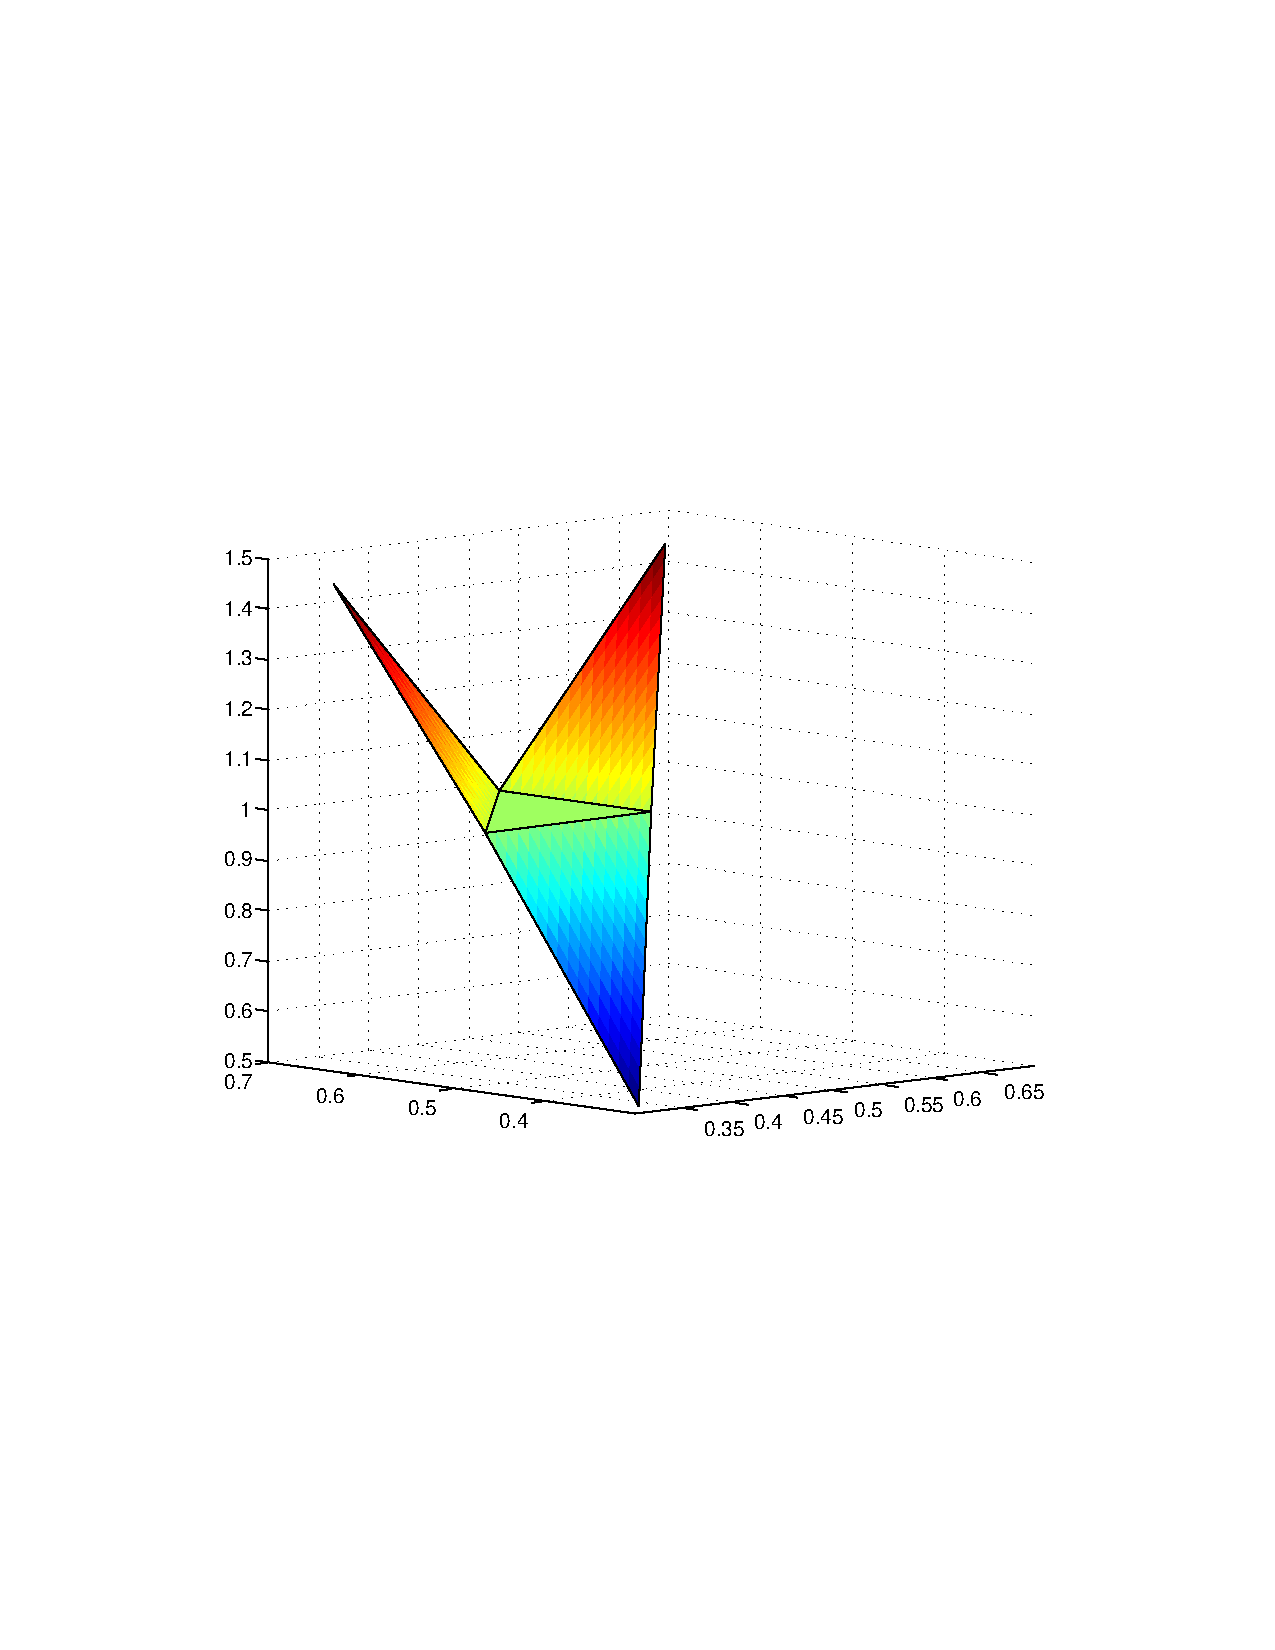
\includegraphics[trim=3cm 8cm 3cm 8cm, width=1.\textwidth]{control_polygon2.pdf}
	\caption{control polygon}
\end{subfigure}
\begin{subfigure}[b]{.5\textwidth}
	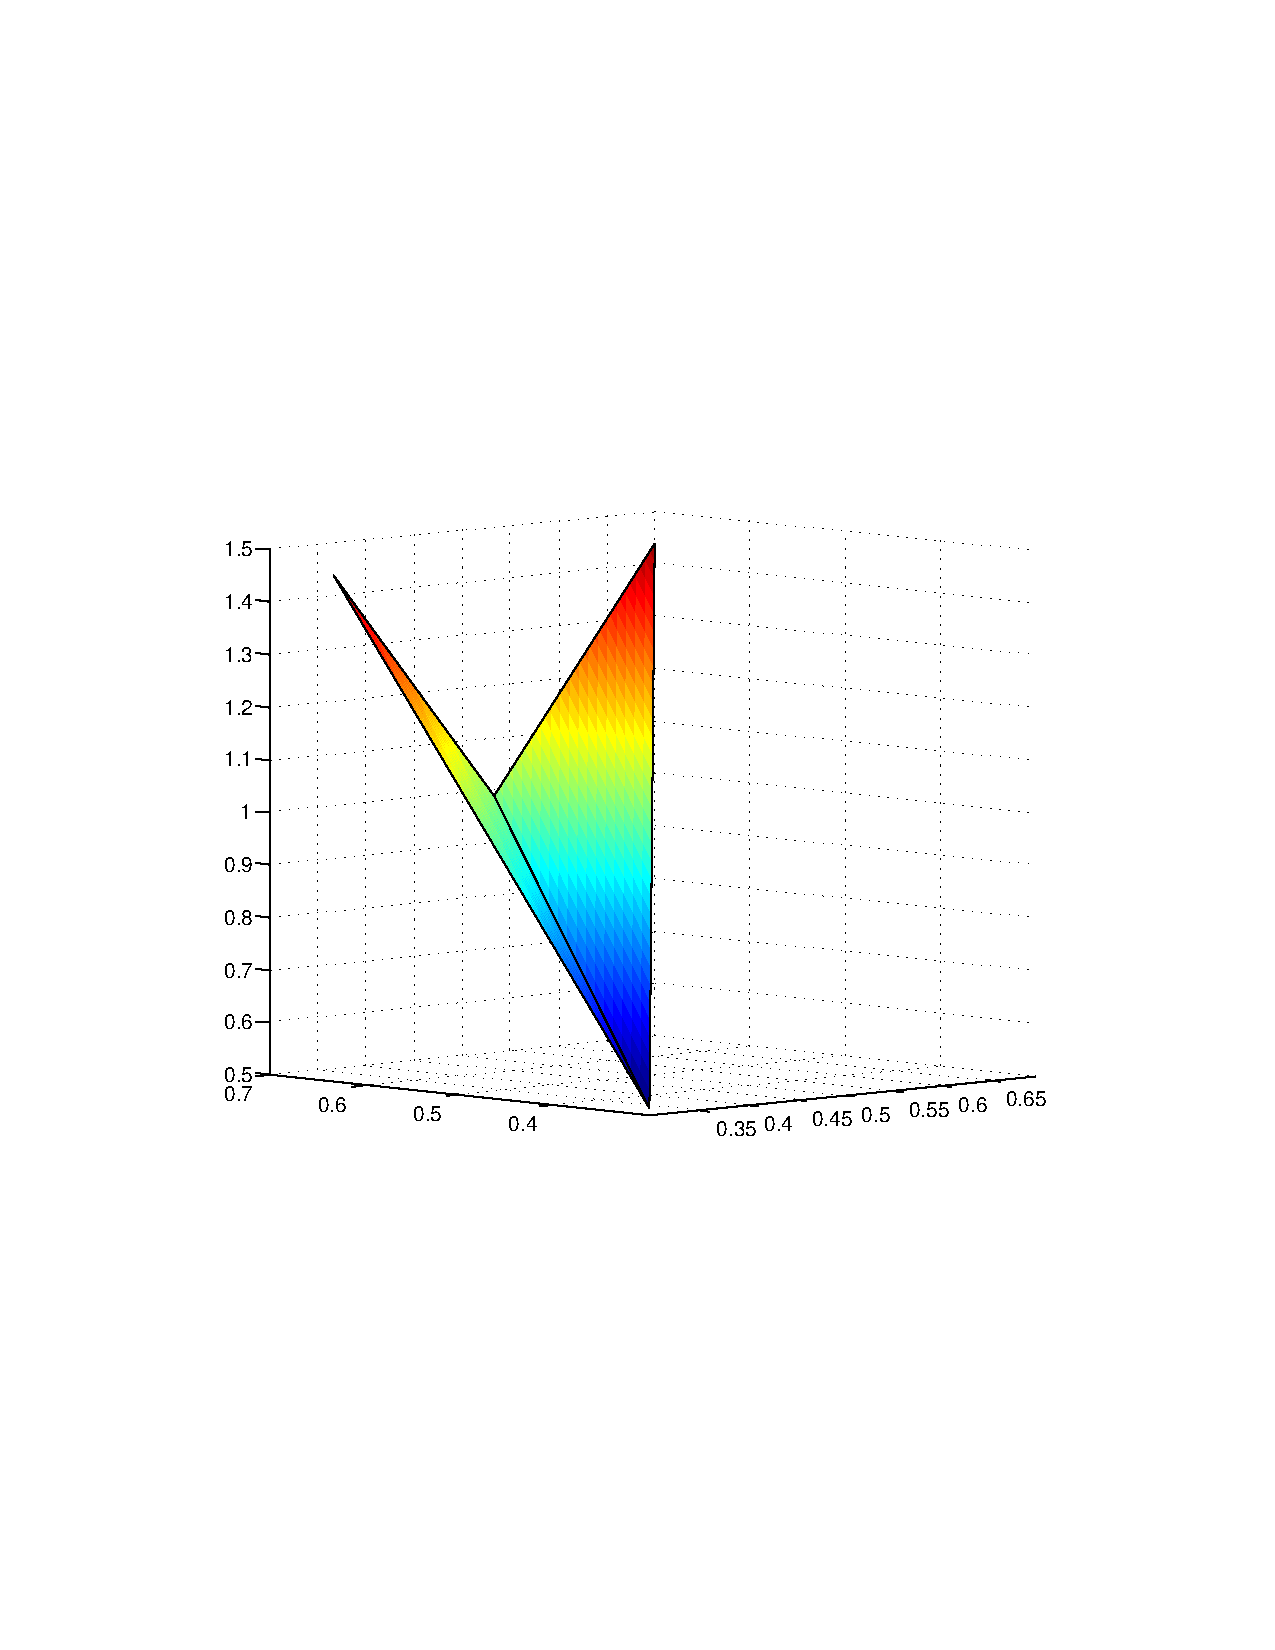
\includegraphics[trim=3cm 8cm 3cm 8cm, width=1.\textwidth]{convex_hull2.pdf}
	\caption{lower convex hull}
\end{subfigure}
\caption{The control polygon and lower convex hull of a given set of control points}
\label{fig: diff connectivity}
\end{figure}

While the the control polygon is obviously not convex, the surface of the lower convex hull of the control points is convex because it connect the inner control points differently.

Schumaker and Speleers present in \cite{SS2014} an approach to ensure convexity by a set of conditions on the coefficents , resulting in a quadratic program with linear constraints. To set up the convexity constraints we first need to define the difference operator
\begin{definition}[Difference Operator]
	$\Delta_{\mu \nu}$ is the \emph{difference operator} along the edge $(v_\mu, v_\nu)$ as for example
	\begin{align*}
		\Delta_{21} c_{ijk} &= c_{i,j+1,k} -c_{i+1, j,k}  \\
		\Delta_{31}^2 c_{ijk} &= c_{i,j,k+2} -2c_{i, j+1,k+1} +c_{i, j+2,k} \\
		\Delta_{12} \Delta_{32} c_{ijk} &= c_{i,j+1,k+1} -c_{i+1, j,k+1} - c_{i,j+2,k} +c_{i+1, j+1,k}\\	\end{align*}
\end{definition}
 
Lai and Schumaker present in \cite{LS2007} \todo{siehe nummer 3 in $C^0 $ schumaker paper} a sufficient condition to ensure convexity on a triangle.
\begin{theorem}[A Sufficient Condition for Convexity]
	A polynomial $p$ is convex on a triangle $T$ if the matrix
	\[
		\begin{pmatrix}
			\Delta_{21}^2 c_{ijk} & \Delta_{31} c_{ijk} \Delta_{32} c_{ijk}\\
			\Delta_{31}c_{ijk} \Delta_{32} c_{ijk} & \Delta_{31}^2 c_{ijk} 
		\end{pmatrix}
	\]
	is nonnegative definite for each $i + j + k =2 $.
\end{theorem}
Note, that this condition is quadratic in the coefficients. But there are many relaxations of these conditions, we refer the interested leader to \cite{SS2010}. \todo{zitate}An example with 12 inequalities is \todo{welche art von satz, theorem, etc?}
\begin{theorem}[Sufficient Linear Conditions for Convexity]
	A polynomial $p$ is convex on a triangle $T$ if its B\'ezier coefficient $c_{ijk}$ satisfy
	\begin{align*}
		&(\Delta_{21} + 2\Delta_{31}) \Delta_{31} c_{ijk} \geq 0, 
		&   (\Delta_{21}^2 + 3\Delta_{21} \Delta_{31} + 2 \Delta_{31}^2) c_{ijk} \geq 0, \\
		& \Delta_{21}(2\Delta_{21} + \Delta_{31})  c_{ijk} \geq 0, 
		&   (2\Delta_{21}^2 + 3\Delta_{21} \Delta_{31} +  \Delta_{31}^2) c_{ijk} \geq 0, \\  
		&(\Delta_{32} + 2\Delta_{12}) \Delta_{12} c_{ijk} \geq 0, 
		&   (\Delta_{32}^2 + 3\Delta_{32} \Delta_{12} + 2 \Delta_{12}^2) c_{ijk} \geq 0, \\
		&\Delta_{32} (2\Delta_{32} + \Delta_{12}) c_{ijk} \geq 0, 
		&   (2\Delta_{32}^2 + 3\Delta_{32} \Delta_{12} +  \Delta_{12}^2) c_{ijk} \geq 0, \\  
		&(\Delta_{13} + 2\Delta_{23}) \Delta_{23} c_{ijk} \geq 0, 
		&   (\Delta_{13}^2 + 3\Delta_{13} \Delta_{23} + 2 \Delta_{23}^2) c_{ijk} \geq 0, \\
		& \Delta_{13}(2\Delta_{13} + \Delta_{23})  c_{ijk} \geq 0, 
		&   (2\Delta_{13}^2 + 3\Delta_{13} \Delta_{23} +  \Delta_{23}^2) c_{ijk} \geq 0   
	\end{align*}
	for all $i + j + k =2 $.
\end{theorem}
The latter conditions only ensure convexity on a single triangle. That would suffice for piecewise polynomials contained $C^1$ because for them unlike to splines contained in $C^0$ convexity on each triangle implies global convexity. To patch this matter Schumaker and Speleers introduce further conditions making sure splines are convex across triangle boundaries//edges, as they prove in Theorem 3.6 \cite{SS2014}.
\begin{theorem}[Sufficient Conditions for Convexity across Triangle Edges]
	Let $p$ be a piecewise polynomial being convex on every triangle. Suppose its B\'ezier coefficients for every interior edge $e =(v_\kappa, v_\mu)$ fulfill 
	\begin{align}
		{\hat c_{i,j,1}} = \beta_1^c c_{i+1, 0,j} +\beta_2^c c_{i,1,j} + \beta_1^c c_{i, 0,j+1}, \; i+j=d-1, \label{eq: convexity across edge}
	\end{align}
where  $\{c_{i,j,k}\}_{i+j+k=d}$ and $\{ {\hat c_{i,j,k}}\}_{i+j+k=d}$ are the B\'ezier coefficients of $p$ relative to the two triangles $T_1 = \langle v_\kappa, v_\lambda, v_\mu \rangle$ and $T_2 = \langle v_\kappa, v_\mu, v_\nu \rangle$ sharing the edge $e$, and $(\beta_1^c,\beta_2^c,\beta_3^c)$ are the barycentric coordinates of $v_\nu$ with respect to $T_1$. Then $p$ is convex.
\end{theorem}

\begin{figure}[h]
			\begin{center}
		\begin{tikzpicture}
%define coordinates
			\coordinate (vEins) at (120:4cm) ;
			\coordinate (vZwei) at (60:4cm);
			\coordinate (vDrei) at (0:0cm);
			\coordinate (vVier) at (0:4cm);

			\draw (0,0) -- (vEins) -- (vZwei) -- node[above left ] {$e$} (vDrei) -- (vVier) -- (vZwei);

%draw nodes
			\draw[fill =black] (vEins) circle (1pt) node[left] {$ v_\nu$};
			\draw[fill =black] (vZwei) circle (1pt) node[right] {$v_\mu$};
			\draw[fill =black] (vDrei) circle (1pt) node[below] {$v_\kappa$};
			\draw[fill =black] (vVier) circle (1pt) node[right] {$v_\lambda$};

%draw control points in T_1
			\draw[fill =blue] ($(vEins)!0.5!(vZwei)$) circle (1pt) node[above] {$\blue{\hat \xi_{011}}$};
			\draw[fill =blue] ($(vEins)!0.5!(vDrei)$) circle (1pt) node[left] {$\blue{\hat \xi_{101}}$};
			\draw[fill =blue] ($(vDrei)!0.5!(vZwei)$) circle (1pt) node[left] {$\blue{\hat \xi_{110}}$};

			\draw[fill =blue] (vEins) circle (1pt) node[above] {$\blue{\hat \xi_{002}}$};
			\draw[fill =blue] (vZwei) circle (1pt) node[above] {$\blue{\hat \xi_{020}}$};
			\draw[fill =blue] (vDrei) circle (1pt) node[below left] {$\blue{\hat \xi_{200}}$};

%draw control points in T_2
			\draw[fill =blue] ($(vVier)!0.5!(vZwei)$) circle (1pt) node [right] {$\blue{\xi_{011}}$};
			\draw[fill =blue] ($(vVier)!0.5!(vDrei)$) circle (1pt) node[below] {$\blue{\xi_{110}}$};
			\draw[fill =blue] ($(vDrei)!0.5!(vZwei)$) circle (1pt) node[right] {$\blue{ \xi_{101}}$};

			\draw[fill =blue] (vZwei) circle (1pt) node[below right] {$\blue{\xi_{002}}$};
			\draw[fill =blue] (vDrei) circle (1pt) node[below right] {$\blue{\xi_{200}}$};
			\draw[fill =blue] (vVier) circle (1pt) node[below] {$\blue{ \xi_{020}}$};

			\draw node at (90:2.2cm) {$T_2$};
			\draw node at (30:2.4cm) {$T_1$};
			
		\end{tikzpicture}
		\end{center}

	\caption{Two triangles}
\end{figure}

For quadratic splines Schumaker and Speleers even prove the inversion on convex domains $\Omega$, namely if for every interior edge its coefficients satisfy \eqref{eq: convexity across edge} then the corresponding spline is convex.
This result does not generalise for higher degrees. In fact they give a counterexample for degree $k = 3$.

Now we apply the new insights//methods to the function given after solving the generalised poisson problem stated in \ref{sec: SIPG}.
Given the DG solution of the generalised poisson problem $u^{gp}_h$ we seek for a convex spline minimising the error at the B\'ezier control points, i.e. we want to find the B\'ezier coefficients $c$ minimising
\[
		\lVert A c - b \rVert_2, \qquad \text{ such that } Cc \geq 0,
\]
where $A$ is the matrix evaluating the to $c$ corresponding piecewise polynomial at the B\'ezier control points, $b$ are the function values of $u^{gp}_h$ at the B\'ezier control points and $C$ is the matrix containing the conditions ensuring convexity on the whole domain.

\subsubsection{Solving the Quadratic Program}
\todo{how to solve the quadratic program}

\subsection{Initial Guess}
Just as the most methods for the \MA equation the fixed point iteration requires an initial guess. Two approaches are very favoured in the literature.
One is to start with the solution of the equation
\begin{align}
	\begin{split}
	\triangledown u &= \sqrt{2f} \text{ in } \Omega \\ 
	u &= g \text{ on }\partial \Omega.
	\end{split}\label{eq: start sqrt_f}
\end{align}

\todo{motivation for this approach}

The other is a nested iteration ansatz. At a the coarsest level $h_1$ one chooses any convex function as initial guess$u^0_{h_1}$, mostly $\frac 1 2 ({x_1^2} + {x_2^2}) $ for it is convex polynomial with a low degree. For finer triangulations $\mathcal{T}_{h_{l}}$ the solution of the previously computed solution $u_{h_{l-1}}$is taken for a starting point.

Advantageously at the first approach is the compliance of the boundary conditions.
The second approach regards the fact that probably the method's robustness decreases for finer meshes.


\section{First Implementation}
At the beginning we implemented the SIPG method exactly as stated in section \ref{sec: SIPG}.
As an initial guess served the solution of \eqref{eq: start sqrt_f} , the penalty parameter was chosen to be 30 and the domain $\Omega$ the unit square$[0,1]^2$.

For first numerical results we consider the rather simple equation
\begin{align}
	\mydet {D^2 u} &= 1 \text{ in } \Omega \\ 
	u &= \frac 1 2 (x_1^2 + x_2^2 )\text{ on }\partial \Omega.	
\end{align}
with the exact classical solution $\frac 1 2 (x_1^2 + x_2^2 )$. However, even for this rather simple example the iteration does not converge. This implementation even fails the consistency check. Given the exact solution as starting point the $L2$ error steadily increases, as shown in figure \ref{fig: consisctency_first_try}
\begin{figure}[h]
	\centering
	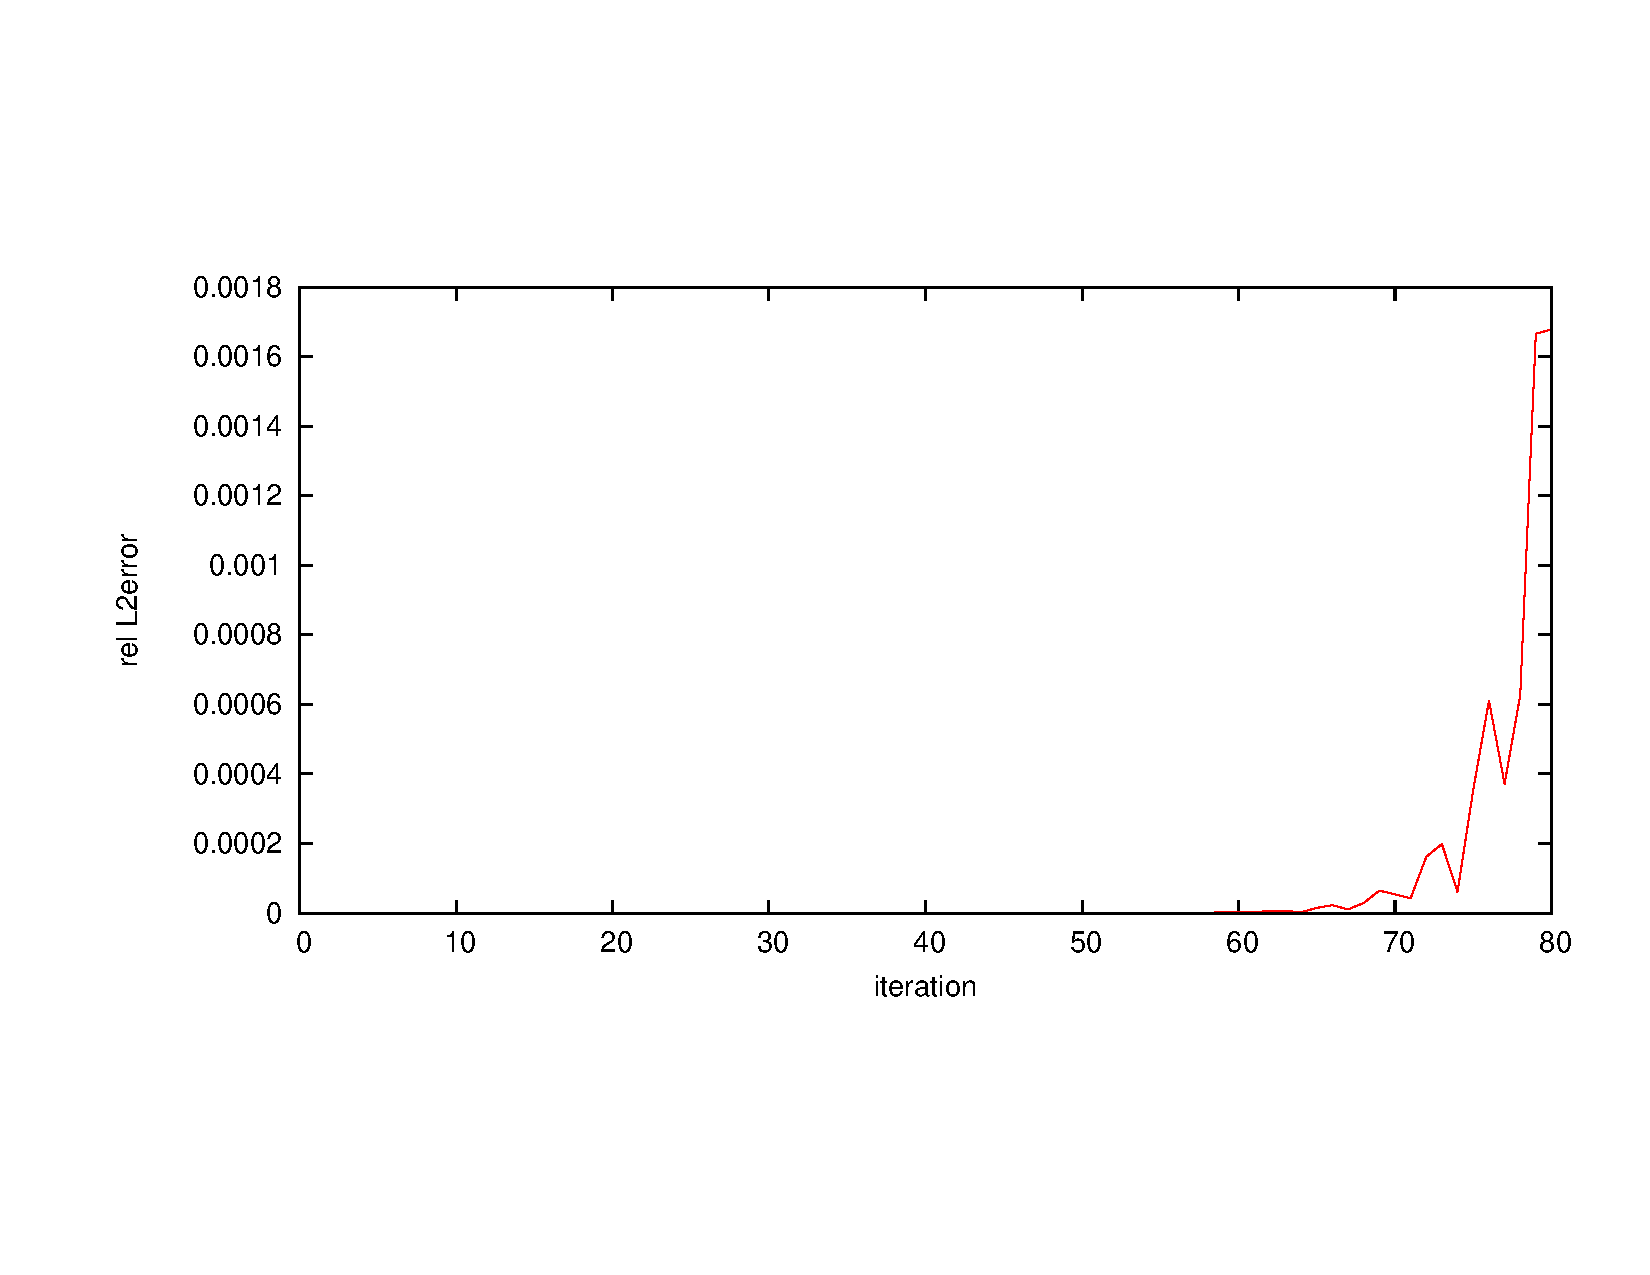
\includegraphics[trim = 2cm 4cm 1cm 4cm, width=1\textwidth]{plots/consisctency_first_try.pdf}
	\caption{Relative $L2$ error on a grid with $h=\frac 1 2$}
	\label{fig: consisctency_first_try}
\end{figure}
Looking at latter steps one is able see in the solution the underlying grid structure. Everywhere a triangle edge lies sharps edges arise. Besides continuity the solution on two triangles seem independent although the exact solution is absolutely  regular.

A similar approach works for quasilinear methods, so it is a good starting to analyse the main difference, i.e. the derivation in the iterated variable. This leads us to the question: How good serves the second derivative of the Poisson solution for an approximation of the exact second derivative?
We illustrate the significance of this question by a example
\begin{example}
	Let $\tilde u$ be an approximation of $u\in C^2(\R)$ with $u-\tilde u \in \bigO(h)$. Differentiating twice we are left with $\dxx{x} u(x)-\dxx{x} \tilde u(x)\in \bigO(h^{-1})$ meaning a decrease of the grid size comes along with a increase of the error in the second derivatives.
	????????//
	 an approximation find
	\begin{align*}
		\dxx{x} u(x)-\dxx{x} \tilde u(x) \approx \frac{\tilde u(x+2h) - 2\tilde u(x) - \tilde u(x-2h) - (u(x+2h) - 2u(x) - u(x-2h))} {4h^2} \\
		 \in \bigO(h^{-1})
	\end{align*}
\end{example}
Let us recall the geometric interpretation of the second derivative, it indicates the curvature of a function and hence also describes the convexity, concavity respectively.

In order to simplify the required calculation we restricted ourselves test space of piecewise polynomials of degree 2. Hence, we receive a piecewise constant Hessian in every step which is especially during the first iterations not smooth.
On one hand one can hope for a smoothing by a convexification for it will smooth away all unintended concave curvatures. But on the other hand the result is still unsatisfiable because convexification does not affect sharp edges at triangle transitions.

\subsection{An additional Penalty Parameter}
Another idea is force more regularity on the first derivative and thus, implicitly obtain a more steady solution. This suits to the ansatz pursued by Neilan described in section \ref{subsec: disrete Hessian}, his proposed correction terms vanish as the gradient jump across internal edges tends to zero.
Hence, we add the following normal derivatives penalty term 
\begin{align}
	\sum_{e \in \edgesi} \sigma_g |e |\int_e \jump{ \nabla u} \jump {\nabla v} \label{eq: grad penalty term}
\end{align}
to the formulation in \eqref{eq: sipg iteration}.
Note, that this is a strong demand on our solution. We implicitly imply that the desired solution is contained in $H^2(\Omega)$, it is not yet clear how this term behaves for less regular solution.
But, indeed with the new penalisation of the gradient the implementation is consistent with the previous example. The consistency check was carried out with the choice $\sigma_g$ equal to $\sigma=30$, as well as for much smaller choices.
\todo{Noelle gluecklich machen querschnitt}

Nevertheless, starting over with the initial guess from \eqref{eq: start sqrt_f} the method is instable and diverges. But the results yet are very remarkable. As shown in figure \ref{fig: oscillation} the error is oscillating while diverging  to infinity.
\begin{figure}[h]
	\centering
	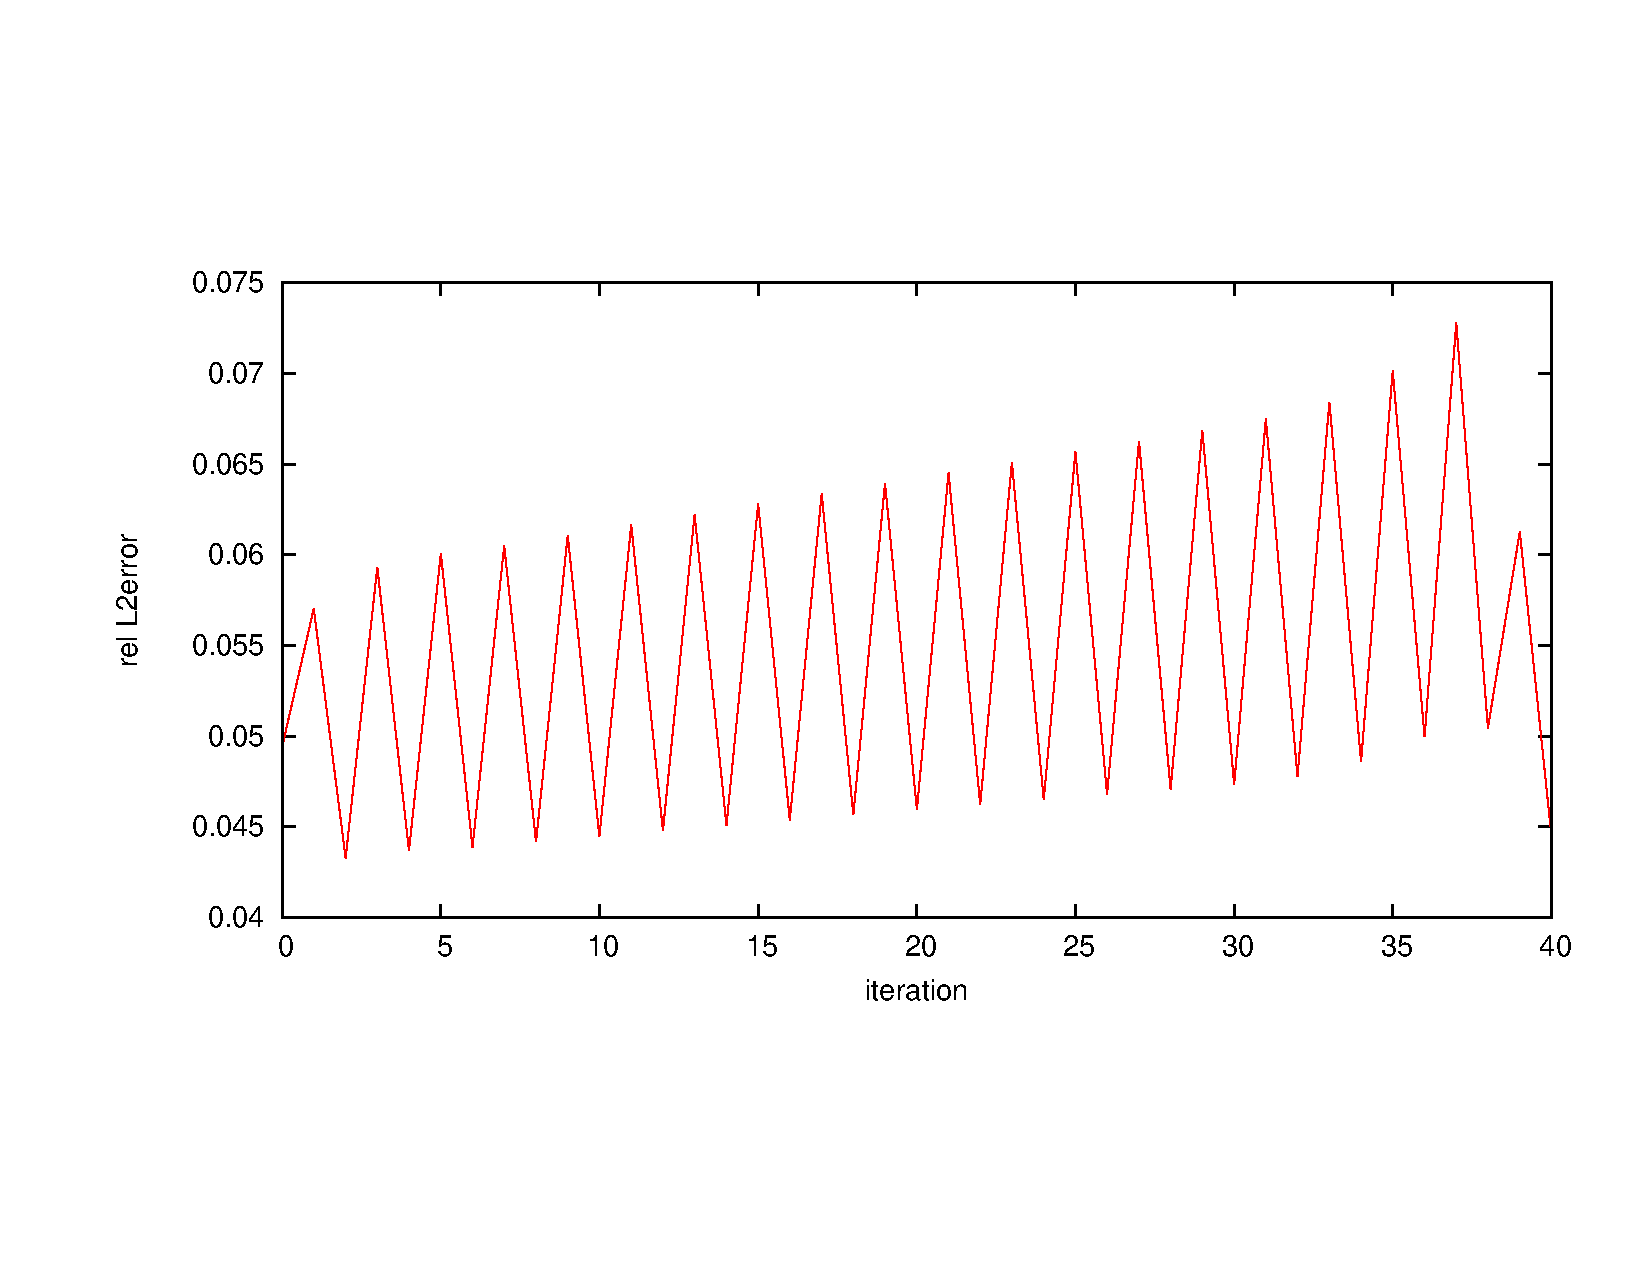
\includegraphics[trim = 2cm 4cm 1cm 4cm, width=1\textwidth]{plots/oscillation.pdf}
	\caption{Relative $L2$ error on a grid with $h=\frac 1 4$ and gradient penalty}
	\label{fig: oscillation}
\end{figure}

\begin{figure}[h]
\begin{subfigure}[b]{.5\textwidth}
	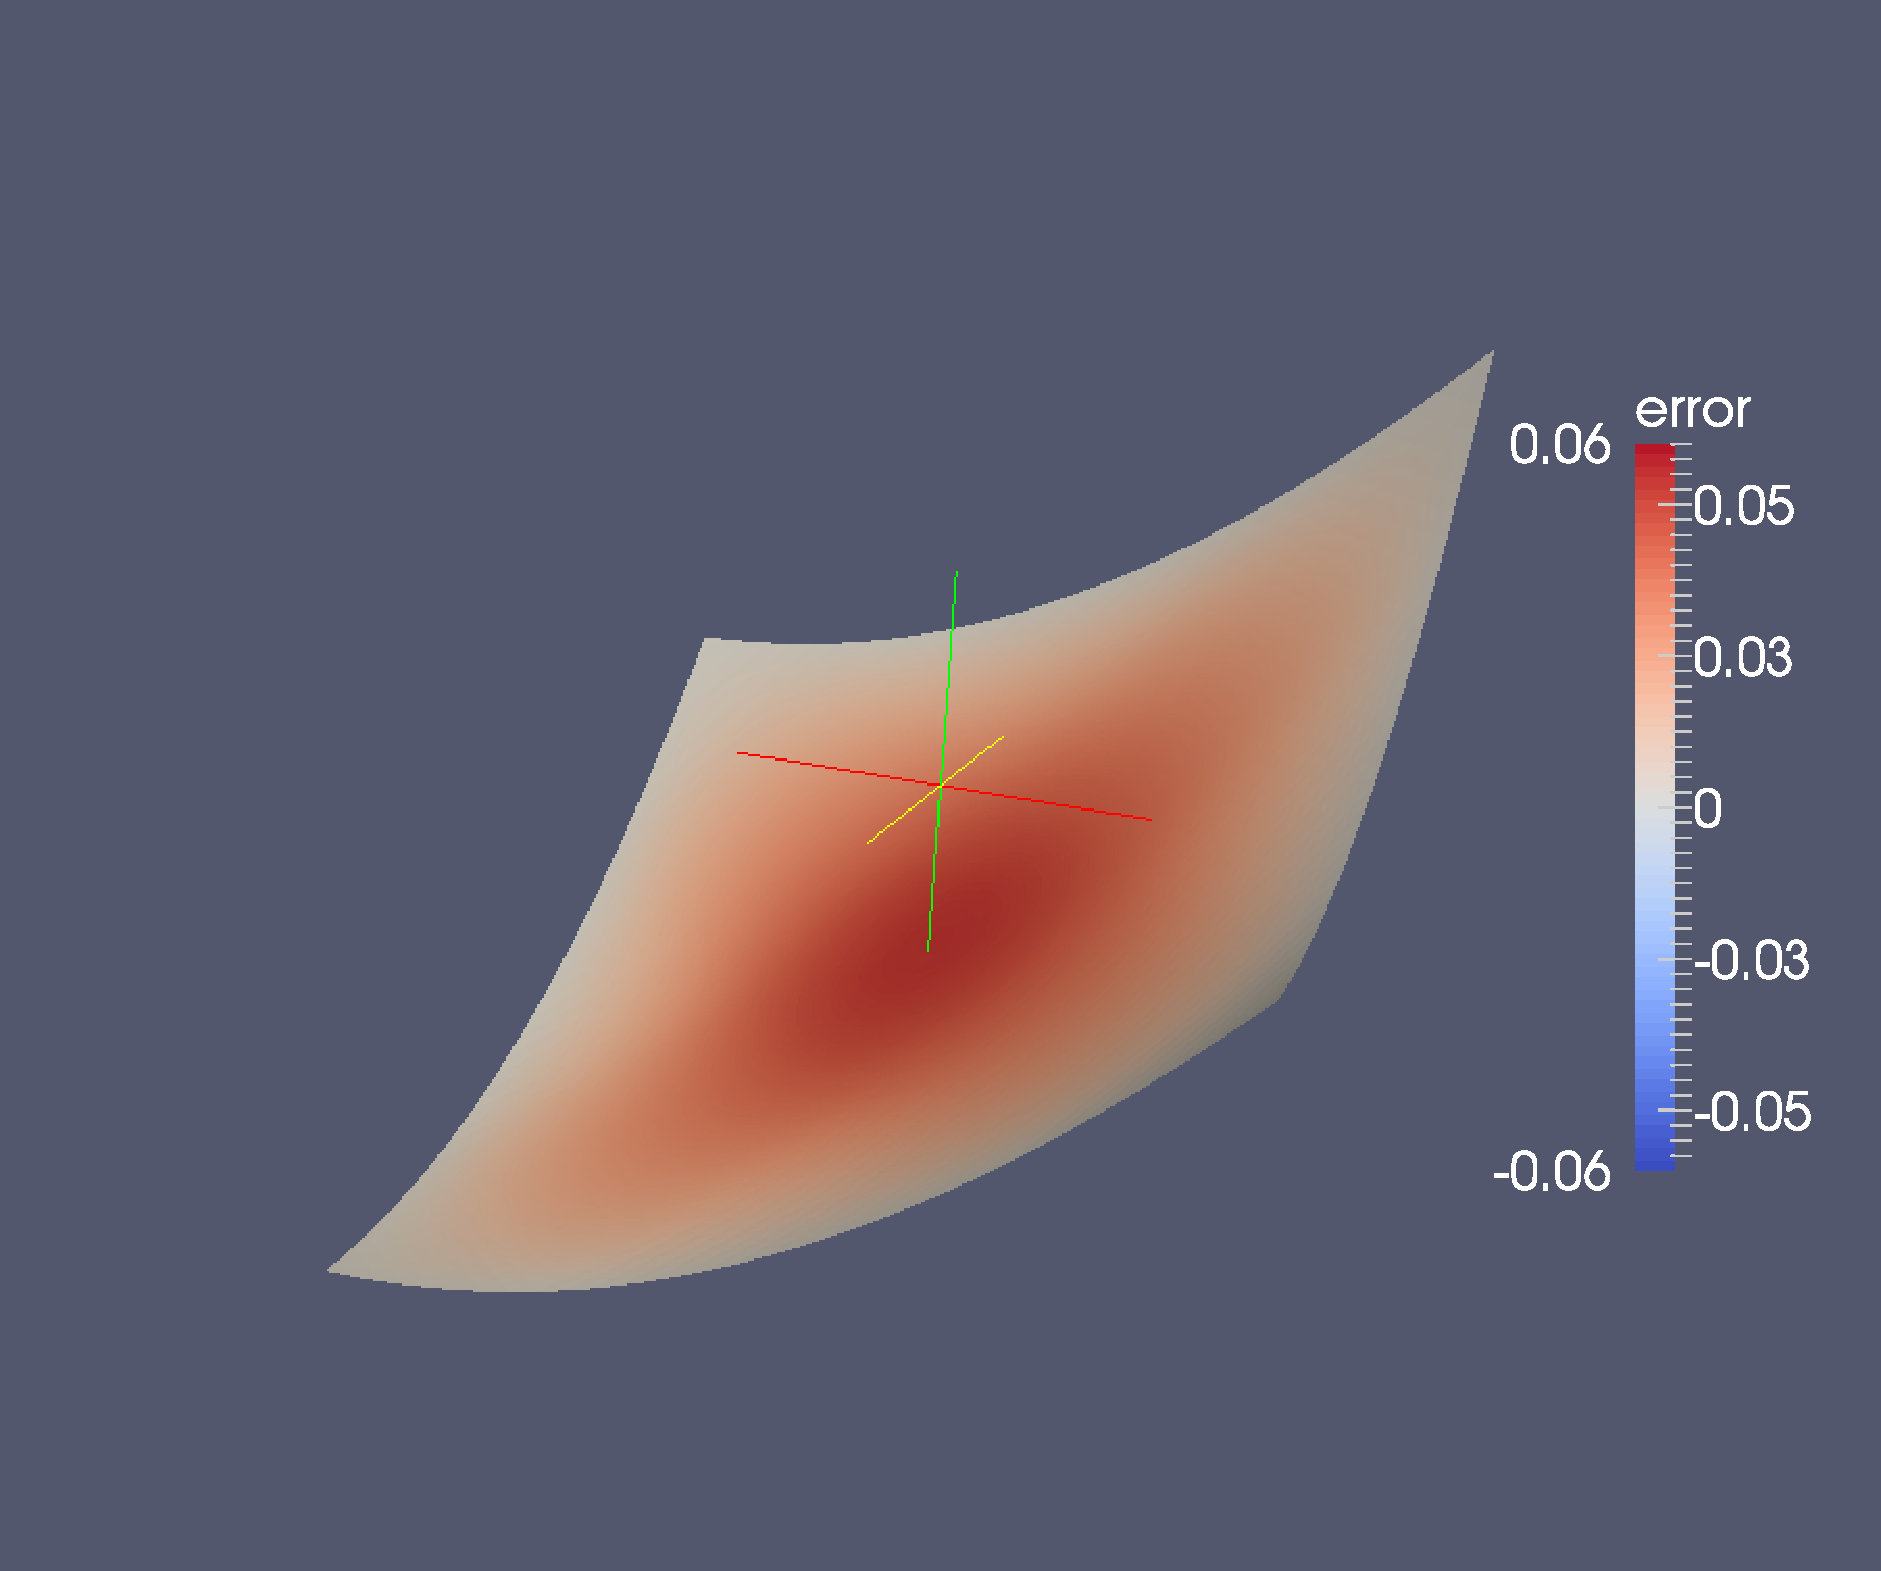
\includegraphics[width=1.\textwidth]{plots/with_penalty_it22.pdf}
	\caption{Solution after 23 steps}
\end{subfigure}
\begin{subfigure}[b]{.5\textwidth}
	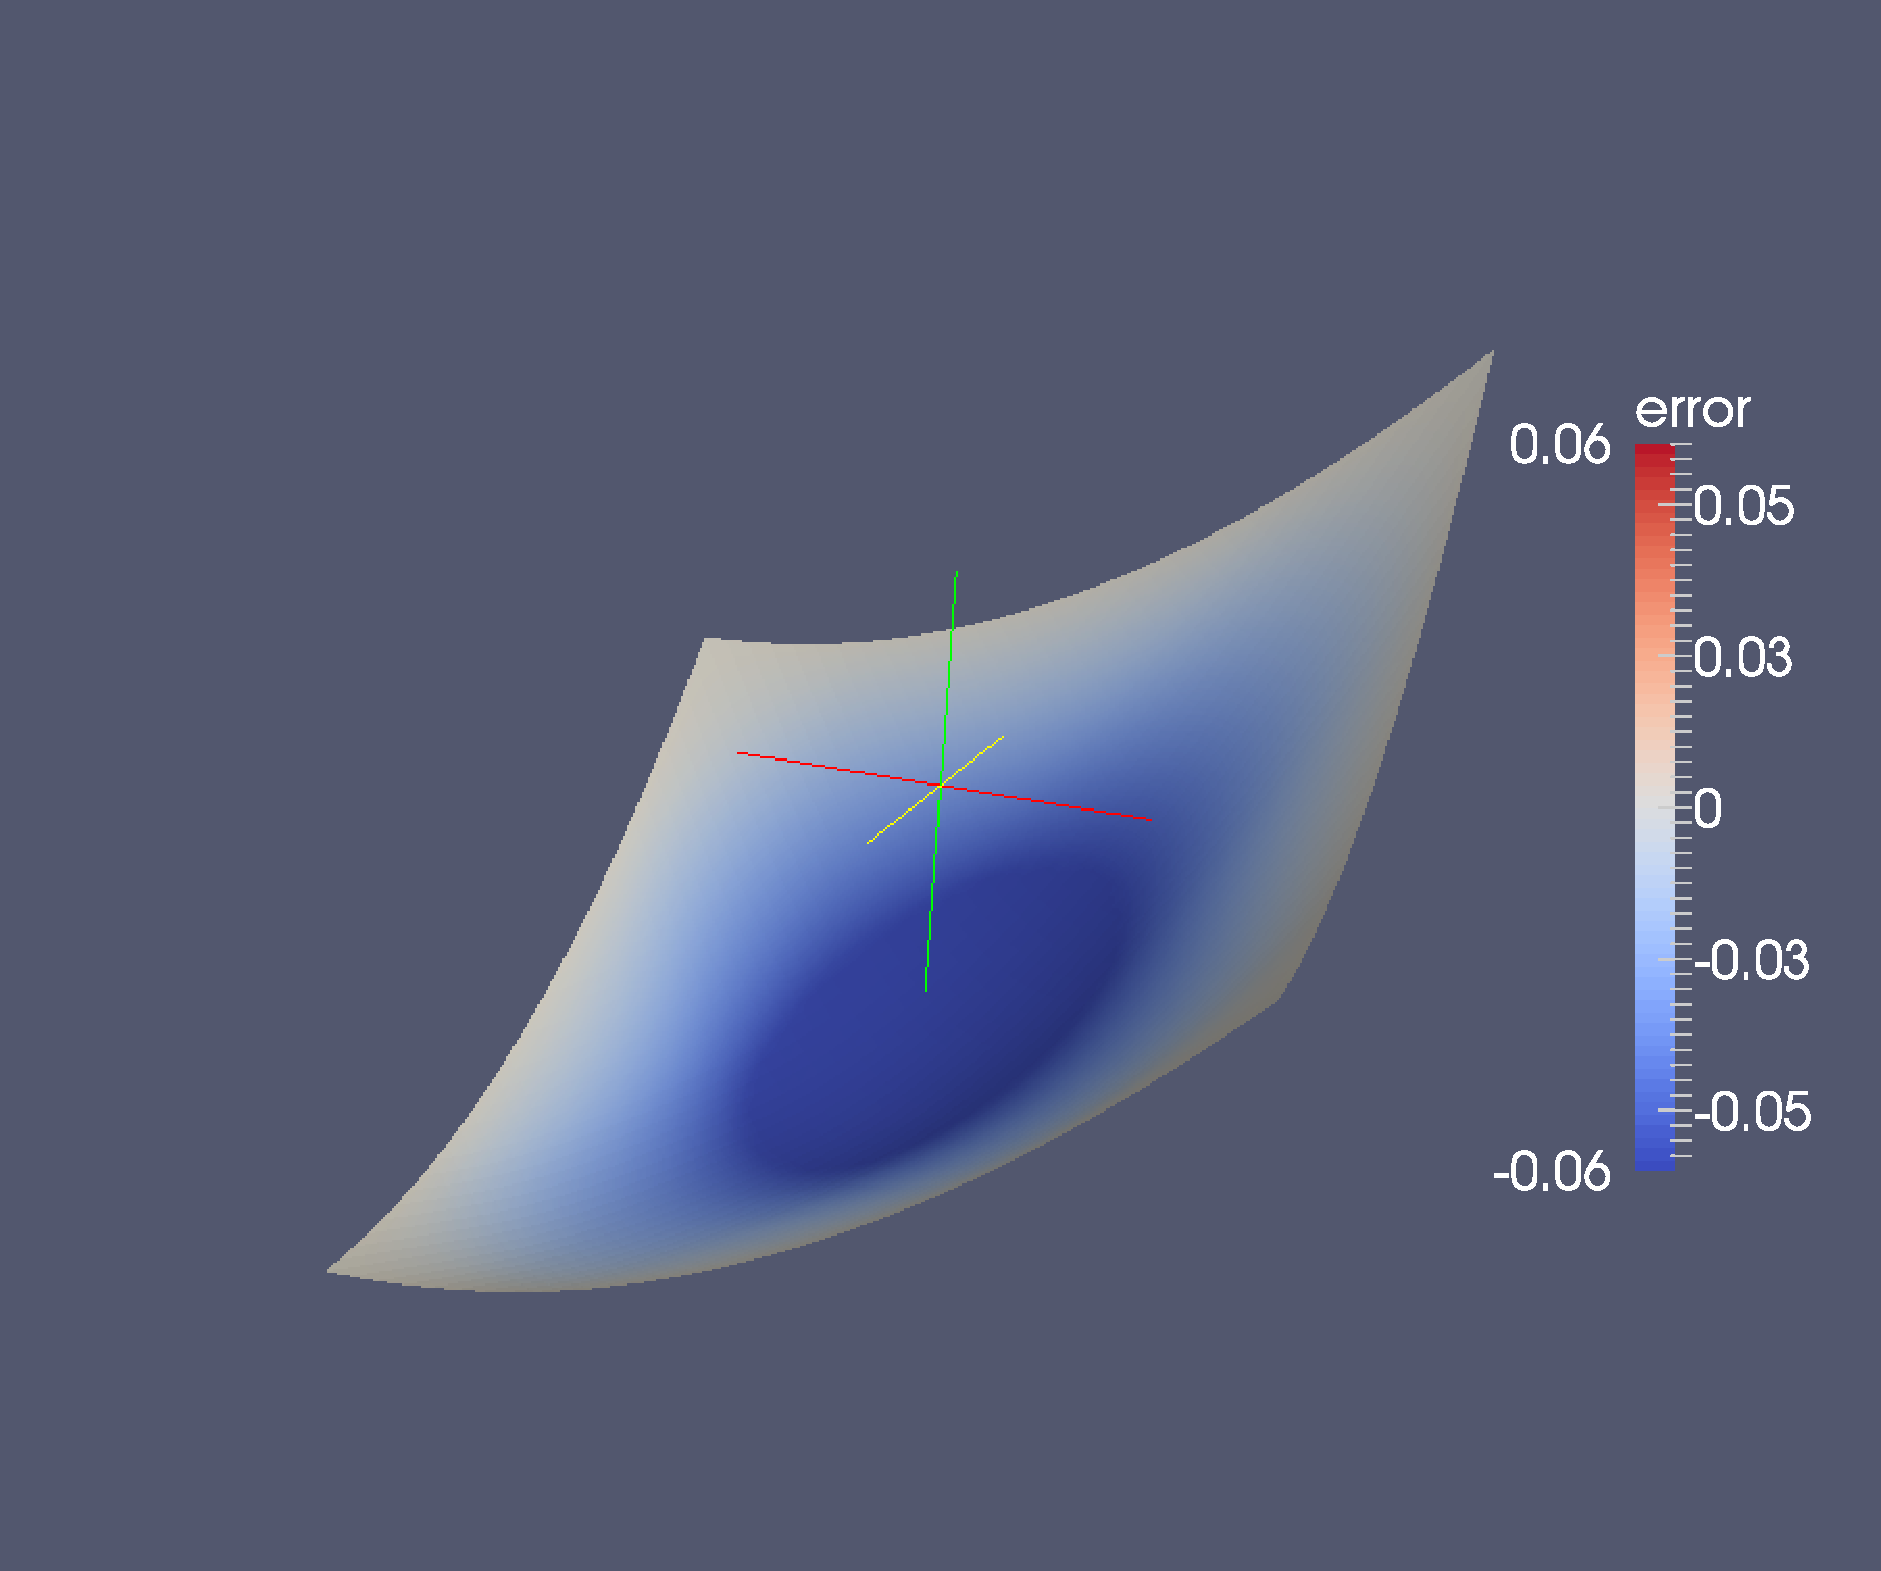
\includegraphics[width=1.\textwidth]{plots/with_penalty_it23.pdf}
	\caption{Solution after 24 steps}
\end{subfigure}
\caption{The solution in two consecutive iterations}
\label{fig: diff iteration}
\end{figure}
Figure \ref{fig: diff iteration} shows to consecutive steps, the error $u-u_{exact}$ is denoted by the surface color. We see that the solution after 23 steps lies above of the exact solution, while one iteration later the Poisson solution lies below of it. These frames are exemplary for the behaviour of our numerical solution. After a step above the solution one below follows, it looks like the solution is split into two subsequences.  And as we have also seen in the devolution of the error, these subsequences seem even to drive each other away from the actual solution.

To prevent our algorithm from doing so we couple the two subsequences by a damping. Before we continue iterating we combine the current solution with the function calculated one step before by an affine composition. Hence we got a further parameter $\alpha$, namely the amount with that the new solution contributes to the iteration.

\section{The final implementation}

\begin{algorithm}
\begin{algorithmic}
\State $u_0\gets $ solution of  $
	\triangle u = \sqrt{2f} \text{ in } \Omega $ with $
	u = g \text{ on }\partial \Omega$
\State $i \gets 1$
\While {$u_i-u_{i-1} < \varepsilon$}
	\State $u_i \gets$ solution of \ref{sec: SIPG}
	\State $u_i \gets \alpha u_{i-1} + (1-\alpha)u_i $
	\State convexify ??????????/
\EndWhile
\end{algorithmic}
\caption{Final Algorithm}
\end{algorithm}
\todo{nested iteration}



\chapter{Numerical Results}
\label{ch:NumericalResults}
%\section{Benchmark Examples}

Since the \MA equation became a benchmark problem for fully nonlinear second order PDEs there are some classical test problems for the two-dimensional case. All test cases are formulate for the domain $\Omega$ to be the unitsquare $[0,1]^2$.

\begin{test} \label{test smooth}
The first classical \MA test is the problem with the data
\[
	u=\exp( \lVert x \rVert_2^2  /2) 
	\text { and } 
	f = (1 + \lVert x \rVert_2^2) \exp( \lVert x \rVert^2).
\]
It has a very smooth solution and is even radial.

\end{test}

\begin{test}\label{test sqrt}
The data
\[
	u = - \sqrt{ 2-  \lVert x \rVert_2^2}
	\text { and } 
	f = 2\left( 2-  \lVert x \rVert_2^2 \right)^{-2}
\]
defines the second example. This test is especially interesting because the convex viscosity solution is only contained in $W^{1,p}(\Omega) $ for $p \in [0,4)$\cite{DG2006a}, i.e. it lacks $H^2$ regularity.
\end{test}

For the next two tests we define $x_0 = \left(\frac 1 2, \frac 1 2  \right)^t$.

\begin{test}\label{test singularity}
The third \MA test is also irregular. Its solution lies in $C^1$ and it is given by
\[
	u=\frac 1 2 \left( \max 0 {\lVert x - x_0 \rVert_2-0.2 }  \right)^2 
	\text { and } 
	f = \max 0 {1-\frac {0.2} {\lVert x - x_0 \rVert_2} }.
\]
\end{test}


\begin{test}\label{test dirac}
The last test is determined by
\[
	u = \lVert x - x_0 \rVert_2
	\text { and } 
	f = \pi \delta_{x_0}
\]
and its solution $u$ describes a cone with origin $x_0$. This example does not have a viscosity solution, but $u$ is only an Aleksandrov solution of the problem \cite[Section 2.3.]{FO2011}.

Note that $f$ is highly non regular. Motivated by \cite[Section 6.1.]{FO2011} we discretise $f$ by
\begin{align*}
	f_h = \begin{cases}
		\frac \pi {4h^2} & \text{ if} \singleNorm{x_1 - 0.5} \leq h \text{ and } \singleNorm{x_e - 0.5} \leq h \\
		0	& \text{otherwise}
	\end{cases}.
\end{align*}
\end{test}


%\begin{test}\label{test rhsConst}
%A test where the analytical solution is unknown is determined by
%\[
%	u = 0 \text{ on } \partial \Omega
%	\text { and } 
%	f = 1
%\]
%defines the last example.
%\end{test}

\section{Numerical Results of a $C^0$ Penalty Method}\label{sec: numerical results brenner}

%read data for case deg=22 and merge into one file
\newcommand{\readDataN}[2]{
\pgfplotstableread{../../FEniCS/data/#1_l2errornorm} #2

\pgfplotstablecreatecol[copy column from table={../../FEniCS/data/#1_h1errornorm}{h1error}] {h1error} #2

\pgfplotstablecreatecol[copy column from table={../../FEniCS/data/#1_newtonSteps}{steps}] {N} #2
}

%\readDataN{MA1_Brenner_deg2}{\MAOneBrennerTwo}
%\readDataN{MA1_Brenner_deg3}{\MAOneBrennerThree}

%\readDataN{MA3_Brenner_deg2}{\MAThreeBrennerTwo}

%\readDataN{MA4_Brenner_deg2}{\MAFourBrennerTwo}
%\readDataN{MA4_Brenner_deg3}{\MAFourBrennerThree}


\readDataN{MA1_Neilan_GradJump_deg22}{\MAOneJumpdegTwoTwo}
\readDataN{MA1_Neilan_GradJump_deg20}{\MAOneJumpdegTwoZero}

\readDataN{MA1_Neilan_deg33}{\MAOnedegThreeThree}
\readDataN{MA1_Neilan_deg32}{\MAOnedegThreeTwo}

%\readDataN{MA2_Neilan_deg22}{\MATwodegTwoTwo}
%\readDataN{MA2_Neilan_deg33}{\MATwodegThreeThree}

%\readDataN{MA3_Neilan_deg22}{\MAThreedegTwoTwo}
%\readDataN{MA3_Neilan_deg33}{\MAThreedegThreeThree}
\readDataN{MA3_Neilan_GradJump_deg22}{\MAThreeJumpdegTwoTwo}
\readDataN{MA3_Neilan_GradJump_deg33}{\MAThreeJumpdegThreeThree}


%\pgfplotstableread{../../FEniCS/data/MA1_Neilan_deg22_l2errornorm} \MAOnedegTwoTwoL
%\pgfplotstableread{../../FEniCS/data/MA1_NeilanGradJump_deg22_l2errornorm} \MAOneJumpdegTwoTwo
%\pgfplotstableread{../../FEniCS/data/MA1_NeilanGradJump_deg22_h1errornorm}\MAOneJumpdegTwoTwoH

%\pgfplotstablecreatecol[copy column from table={../../FEniCS/data/MA1_NeilanGradJump_deg22_h1errornorm}{h1error}] {h1error} \MAOneJumpdegTwoTwo
%\pgfplotstablecreatecol[copy column from table={../../FEniCS/data/MA1_NeilanGradJump_deg22_newtonsteps}{steps}] {N} \MAOneJumpdegTwoTwo


For reference I implemented the algorithm introduced in Section \ref{sec: Brenner method}.
We implemented their presented method using the finite element tool FEniCS \cite{FEniCS}, the Code is append in Appendix \ref{app: Code Brenner}. 
To create our initial guess I did not use a vanishing moment method as Brenner suggested, but the solution of $\triangle u = -\sqrt{2f}$ as introduced in Section \ref{sec: initial guess}. 

The triangulation $\triang$ was obtained by a standard refinement as explained in Section ref{subsec: refinement and base cells}: First the domain was split into four triangles by drawing both diagonals and afterwards each triangle was successively divided into four congruent triangles.
\begin{figure}[H]
	\centering
	\begin{subfigure}{0.45\textwidth}
		\centering
		\edef \n {2}
		\usetikzlibrary{calc}
\begin{tikzpicture}[scale=5]

	\draw (0,0) -- (1,0) -- (1,1) -- (0,1) -- cycle;

	\foreach \x in {0,1,...,\n}
{
	\pgfmathtruncatemacro \y {1-\x/\n}
	\draw (0,\x/\n) -- (1-\x/\n,1);
	\draw (\x/\n,0) -- (1,1-\x/\n);

	\draw (0,\x/\n) -- (\x/\n,0);
	\draw (1,\x/\n) -- (\x/\n,1);

   \draw (\x/\n, \x/\n) -- (1-\x/\n, \x/\n) -- (1-\x/\n, 1-\x/\n) -- (\x/\n, 1- \x/\n) -- cycle;
	\def \y {\x/2/\n}
   \draw (\y, \y) -- (1-\y, \y) -- (1-\y, 1-\y) -- (\y, 1- \y) -- cycle;
}

\end{tikzpicture}
		\caption{Triangulation with $h=\frac 1 2$}
		\label{fig: grid1}
	\end{subfigure}
	\begin{subfigure}{0.45\textwidth}
		\centering
		\edef \n {4}
		\usetikzlibrary{calc}
\begin{tikzpicture}[scale=5]

	\draw (0,0) -- (1,0) -- (1,1) -- (0,1) -- cycle;

	\foreach \x in {0,1,...,\n}
{
	\pgfmathtruncatemacro \y {1-\x/\n}
	\draw (0,\x/\n) -- (1-\x/\n,1);
	\draw (\x/\n,0) -- (1,1-\x/\n);

	\draw (0,\x/\n) -- (\x/\n,0);
	\draw (1,\x/\n) -- (\x/\n,1);

   \draw (\x/\n, \x/\n) -- (1-\x/\n, \x/\n) -- (1-\x/\n, 1-\x/\n) -- (\x/\n, 1- \x/\n) -- cycle;
	\def \y {\x/2/\n}
   \draw (\y, \y) -- (1-\y, \y) -- (1-\y, 1-\y) -- (\y, 1- \y) -- cycle;
}

\end{tikzpicture}
		\caption{Triangulation with $h=\frac 1 4$}
		\label{fig: grid}
	\end{subfigure}	
	\caption{Triangulation with $h=\frac 1 4$}
	\label{fig: grids}
\end{figure}

The arising nonlinear system is solved by PETSc configured with FEniCS default solver choice: That is a Newton based nonlinear solver that uses a line search and the arising linear systems are solved by a $LU$ decomposition.
%SNES Object: 1 MPI processes
%  type: newtonls
%  SNES has not been set up so information may be incomplete
% maximum iterations=10, maximum function evaluations=2000
% tolerances: relative=1e-09, absolute=1e-08, solution=1e-16
%total number of linear solver iterations=0
%total number of function evaluations=0
%SNESLineSearch Object:   1 MPI processes
% type: bt
%  interpolation: cubic
%   alpha=1.000000e-04
%  maxstep=1.000000e+08, minlambda=1.000000e-12
%   tolerances: relative=1.000000e-08, absolute=1.000000e-15, lambda=1.000000e-08
%  maximum iterations=40
%KSP Object:   1 MPI processes
%type: preonly
%maximum iterations=10000, initial guess is zero
% tolerances:  relative=1e-05, absolute=1e-50, divergence=10000
% left preconditioning
% using DEFAULT norm type for convergence test
%PC Object:   1 MPI processes
%  type: lu
%  PC has not been set up so information may be incomplete
%  LU: out-of-place factorization
%   tolerance for zero pivot 2.22045e-14
%   matrix ordering: nd
% linear system matrix = precond matrix:
% Matrix Object:     1 MPI processes
%  type: seqaij
%  rows=112, cols=112
%  total: nonzeros=2744, allocated nonzeros=2744
%  total number of mallocs used during MatSetValues calls =0
%  using I-node routines: found 80 nodes, limit used is 5
Only the absolute tolerance and the number of maximum iteration are changed from the original default values, the absolute tolerance is adjusted to $1e-8$ and the number of maximum iteration restricted to 100. 

The results can be found in figure \ref{fig: Brenner test1} and in table \ref{tab: l2 errors test 1 Brenner} where $h$ denotes the grid width and $N$ denotes the iterations needed to reach the desired tolerance. 

\begin{table}[H]
	\begin{subtable}[b]{0.45\textwidth}
		\centering
		\pgfplotstabletypeset[columns={iterations, l2error, h1error,N},
				    every row 0 column 0/.style={set content=init},
		]\MAOneBrennerTwo
    	\caption{Error for $k=2$}
   \end{subtable}
   ~
	\begin{subtable}[b]{0.45\textwidth}
		\centering
		\pgfplotstabletypeset[columns={iterations, l2error, h1error,N},
				    every row 0 column 0/.style={set content=init},
		]\MAOneBrennerThree
 	\caption{Error for $k=3$}
	\end{subtable}
	\caption{Errors for test case \ref{test smooth}}
	\label{tab: l2 errors test 1 Brenner}
\end{table}

Fitting the data we can calculate the numerical convergence order $2.502$ for $k=2$ and $3.584$ for $k=3$ in the $L^2$ error norm as well as $2.007$ for $k=2$ and $3.028$ in the $H^1$ error norm. Thus, the results in the $H^1$ confirm the almost convergence rate $k$ as predicted by the authors (cf. also Theorem \ref{thm: error estimate brenner}).
Additionally we observe that the method also converges for polynomial degree $k=2$ with optimal rates although the prove of the error estimate do not cover the case $k<3$.

\begin{figure}[H]
\centering
	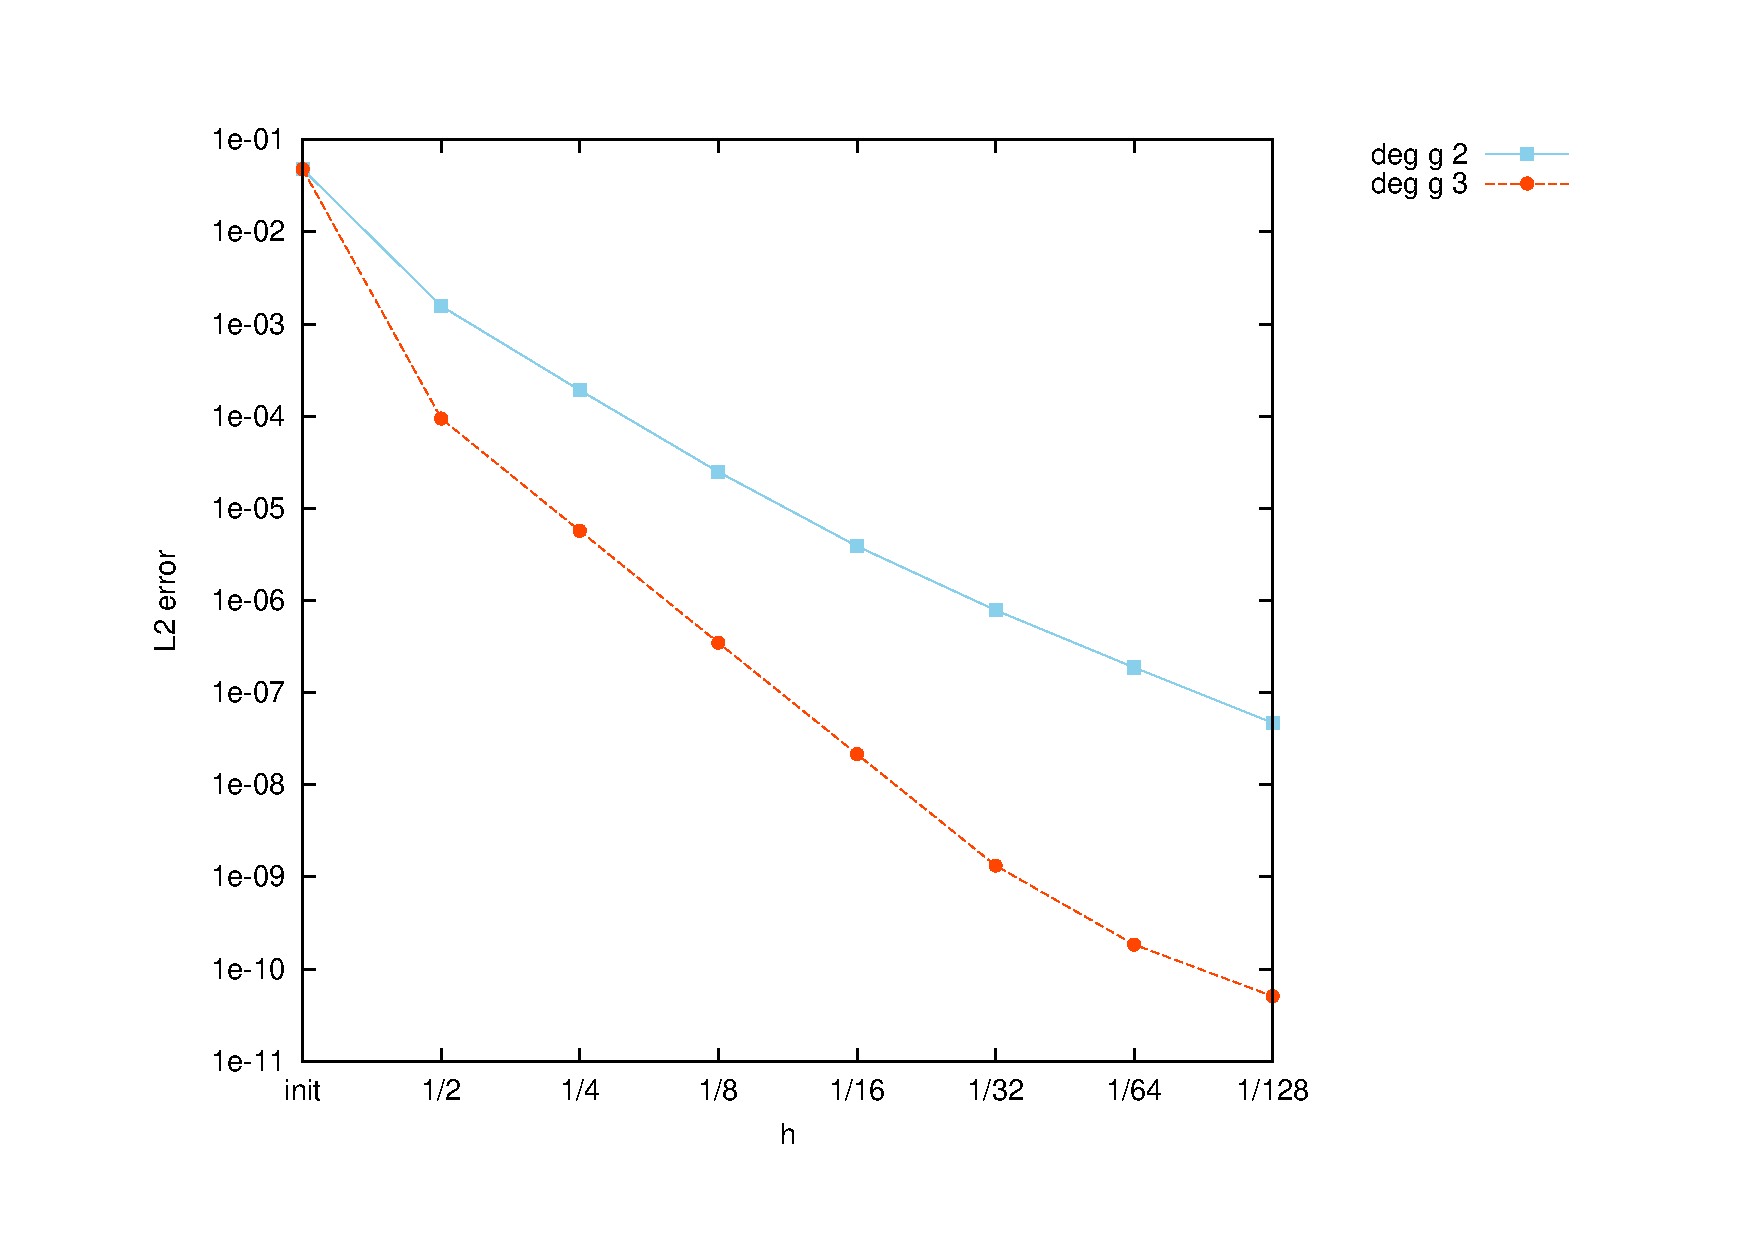
\includegraphics[scale=0.45]{plots/MA1_Brenner_l2.pdf}
	\caption{$L^2$ errors for test case \ref{test smooth}}
	\label{fig: Brenner test1}
\end{figure}
\begin{figure}[H]
	\centering
	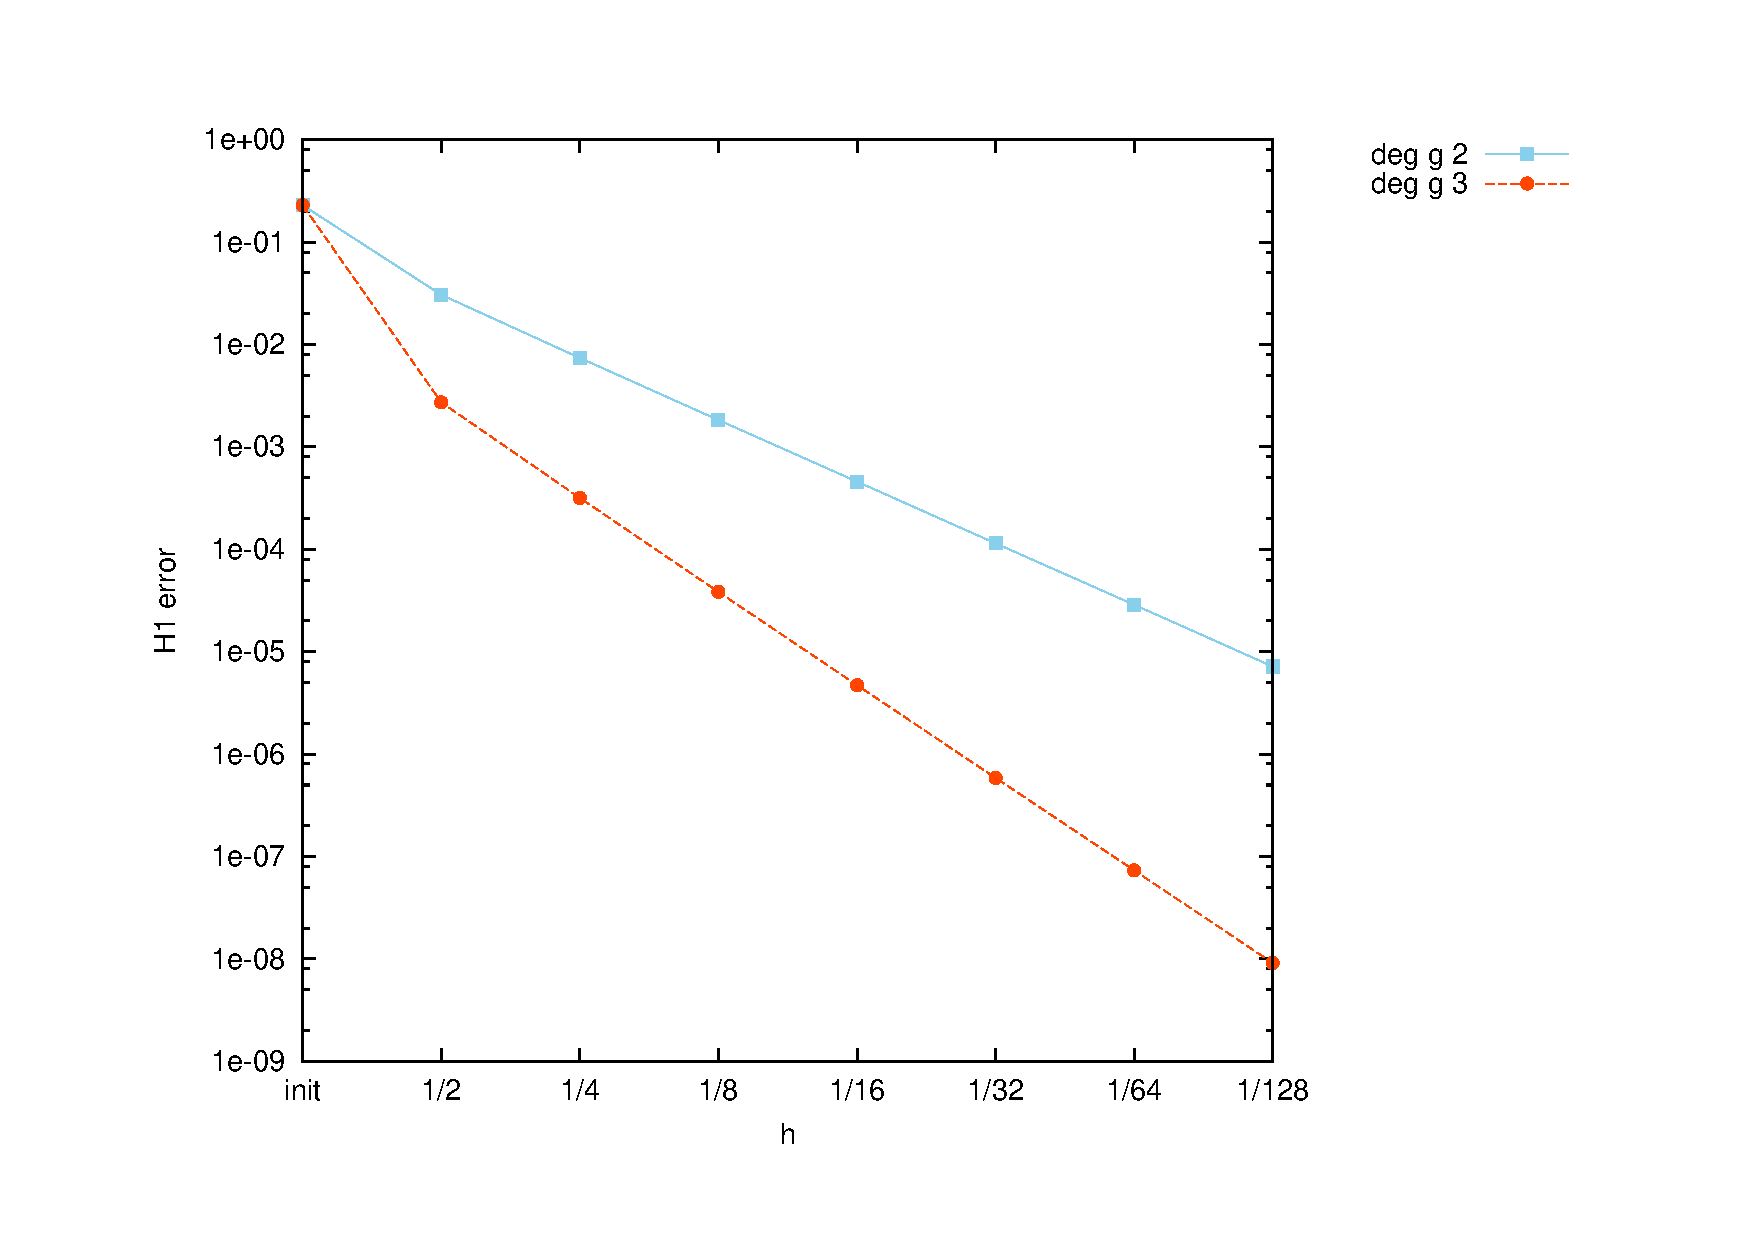
\includegraphics[scale=0.45]{plots/MA1_Brenner_h1.pdf}
	\caption{$H^1$ errors for test case \ref{test smooth}}
	\label{fig: Brenner test1 h1}
\end{figure}

For the second test case the Newton did not converge, not even on the coarsest grid. Also in the third test case our Newton solver had problems. You can see results of the runs for $h=1/2, \dots, 1/16$ in table \ref{tab: l2 errors test 3 Brenner}, for finer grid the solver did not converge. Attempts to solve this example with FEniCS' built in damped Newton method with different relaxation parameters did also not succeed on any grid finer than $1/16$.
\begin{table}[h]
		\centering
		\pgfplotstabletypeset[columns={iterations, l2error, h1error,N},
				    every row 0 column 0/.style={set content=init},
		]\MAThreeBrennerTwo
    	\caption{Error for $k=2$}
	\caption{Errors for test case \ref{test singularity}}
	\label{tab: l2 errors test 3 Brenner}
\end{table}

The fourth example does not have not a classical solution. As in the previous cases the method does not converge. The corresponding results are shown in table \ref{tab: l2 errors test 4 Brenner}.

\begin{table}[H]
	\begin{subtable}[b]{0.45\textwidth}
		\centering
		\pgfplotstabletypeset[columns={iterations, l2error, h1error,N},
				    every row 0 column 0/.style={set content=init},
				    columns/l2error/.style={ /pgf/number format/sci precision=6}     % print 14 digits
		]\MAFourBrennerTwo
    	\caption{Error for $k=2$}
   \end{subtable}
   ~
	\begin{subtable}[b]{0.45\textwidth}
		\centering
		\pgfplotstabletypeset[columns={iterations, l2error, h1error,N},
				    every row 0 column 0/.style={set content=init},
				    columns/l2error/.style={ /pgf/number format/sci precision=6}     % print 14 digits
		]\MAFourBrennerThree
 	\caption{Error for $k=3$}
	\end{subtable}
	\caption{Errors for test case \ref{test dirac}}
	\label{tab: l2 errors test 4 Brenner}
\end{table}

%For the last test case with constant right-hand side and zero Dirichlet boundary data Newton's method only converged on the coarsest grid such that we cannot make any statement on this test.

We see that this method behaves well for smooth solutions for which it was designed. The results show that it is inappropriate for problems with non smooth-solution or viscosity solutions.

\section{Numerical Results of a Finite Element Method based on a Disrete Hessian}\label{sec: numerical results neilan}

Also the Neilan's algorithm \cite{Neilan2014} introduced in Section \ref{sec: FEM discrete Hessian} was implemented.
Additional to the numerical results on convergence which Neilan already presented it is interesting to explore what happens if we vary the polynomial degree for the Hessian ansatz space. 

The implementation was also done with the Finite Element Tool FEniCS \cite{FEniCS}, the corresponding source code can be found in the appendix \ref{app: Code Neilan}. \\
The uniform triangulation $\triang$ is the same as in the scenarios for the $C^0$ penalty method (cf. Section \ref{sec: numerical results brenner})
Different to the initial guess suggested in \cite{Neilan2014} I used the solution of $\triangle u = -\sqrt{2f}$ as introduced in Section \ref{sec: initial guess}. All results presented base on discontinuous ansatz spaces, namely piecewise polynomial spaces as introduced in \ref{def: piecewise polySpace}.

We denote the degree of the trial space $V_h=\mathcal P_h^k$ by $k$ and the degree chosen for the Hessian ansatz space $\Sigma_h = [\mathcal{P}_h^{k_{DH}}]^{d \times d}$ by $k_{DH}$. The solver for nonlinear system of equations given by \eqref{eq: neilan eq1} and \eqref{eq: discrete hessian} or \eqref{eq: neilan eq1 + jump} and \eqref{eq: discrete hessian} is configured with the same paramters as in the previous section if not stated otherwise. 


Figure \ref{fig: l2 errors test 1} shows the $L^2$ error of all performances of the first test case that have converged, the polynomial degrees $k$ were taken to be $1,\dots,3$ and $k_{DH}$ equal to all variants $0, \dots, k$. In Figure \ref{fig: h1 errors test 1} the corresponding $H^1$ errors are plotted.

Due to the large number of degree of freedoms the requested memory for the cases $k=2,3$ and $k_{DH}=2,3$ on the finest grid, for $k=3$ and $k_{DH}=3$ all meshes with $h\geq 1/64$ is too much. Replacing the linear solver by different iterative solvers\footnote{GMRES with an algebraic multigrid preconditioner, GMRES with an incomplete $LU$ factorisation, GMRES with Jacobi preconditioning, bicgstab with preconditioning} yielded to divergence of either the Newton or the linear solver.

\begin{figure}[H]
\centering
	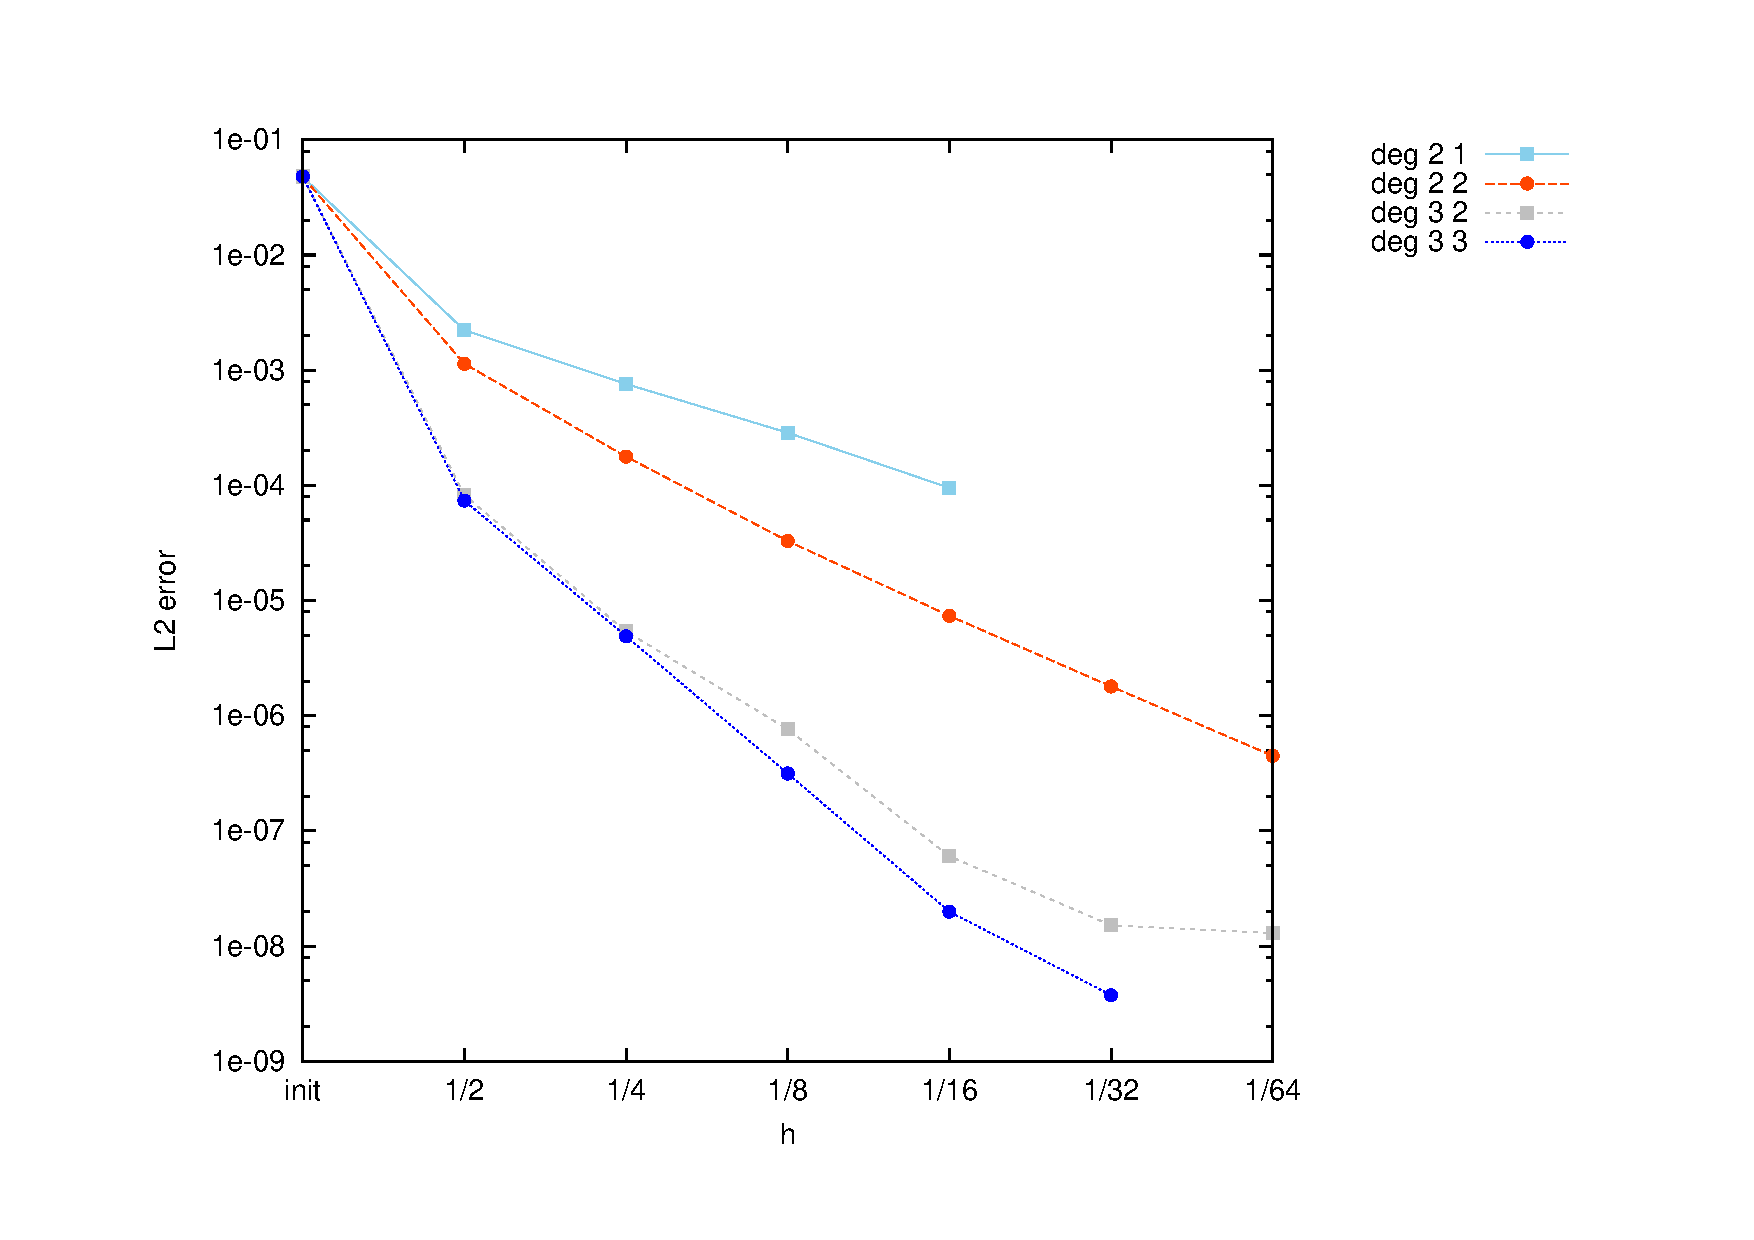
\includegraphics[scale =0.45]{plots/MA1_Neilan_l2.pdf}
	\caption{$L^2$ errors for test case \ref{test smooth}}
	\label{fig: l2 errors test 1}
\end{figure}
The results for the runs with $k=3$ are shown more detailed in Table \ref{tab: l2 errors test 1 deg 2}, in both tables the column $N$ refers to the number of iterations the Newton solver needed to reach the desired tolerance. 
\begin{table}[H]
	\begin{subtable}[b]{0.45\textwidth}
		\centering
		\pgfplotstabletypeset[columns={iterations, l2error, h1error,N},
		every row 0 column 0/.style={set content=init},
		every row 6 column 1/.style={set content=-},
		every row 6 column 2/.style={set content=-},
		every row 6 column 3/.style={set content=-},
		]\MAOnedegThreeThree
		\caption{Error for $k=3, k_{DH}=3$}
	\end{subtable}
	~
	\begin{subtable}[b]{0.45\textwidth}
		\centering
		\pgfplotstabletypeset[columns={iterations, l2error, h1error,N},
		every row 0 column 0/.style={set content=init},
		]\MAOnedegThreeTwo
		\caption{Error for $k=3, k_{DH}=2$}
	\end{subtable}
	\caption{Errors for test case \ref{test smooth}}
	\label{tab: l2 errors test 1 deg 2}
\end{table}


\begin{figure}[H]
\centering
	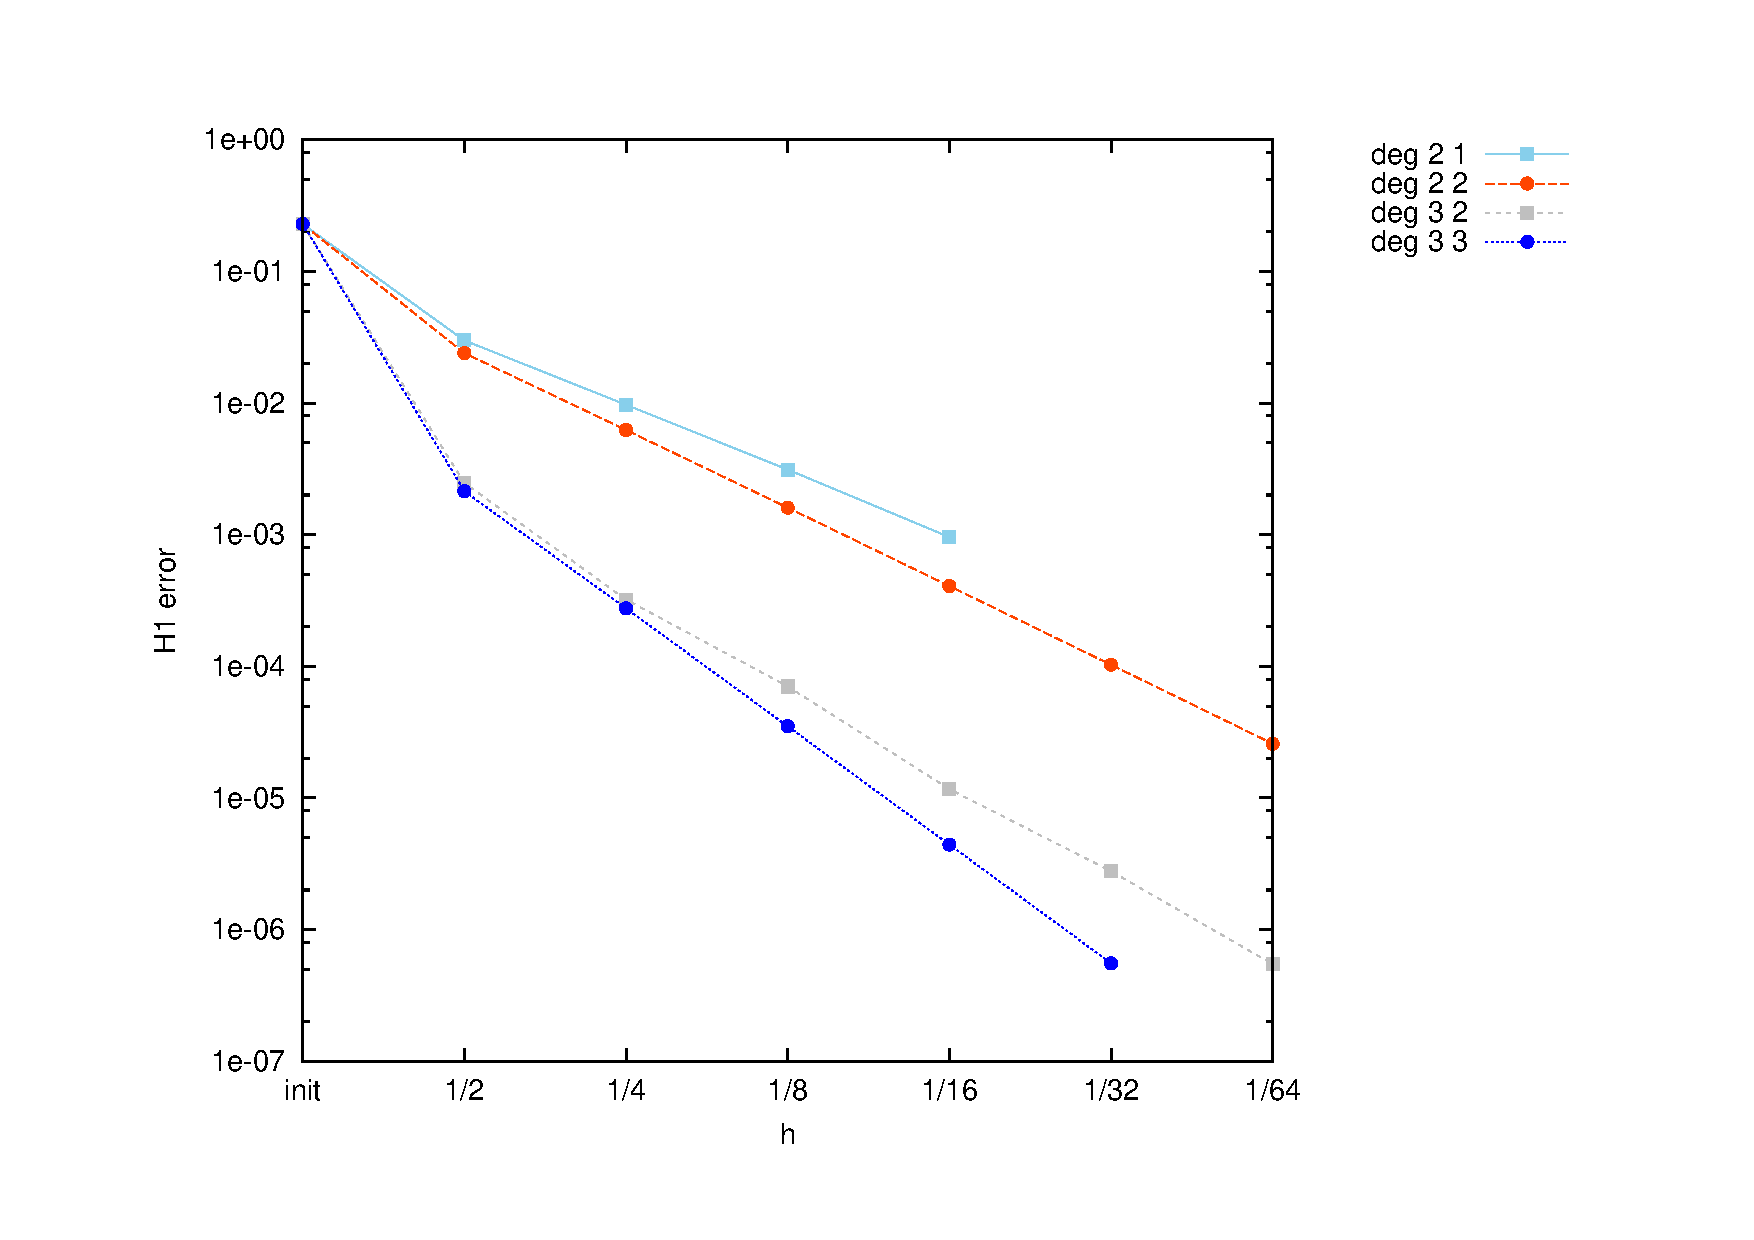
\includegraphics[scale =0.45]{plots/MA1_Neilan_h1.pdf}
	\caption{$H^1$ errors for test case \ref{test smooth}}
	\label{fig: h1 errors test 1}
\end{figure}

As also experienced by Neilan the method does not work for the polynomial degree $k=1$. Similarly, in runs with a low polynomial degree $k_{DH}$ Newton's method did not converge.
Considering this results in the smooth test scenario we observe that the error almost do not alter for different polynomial degrees $k_{DH}$ if both converge. Albeit for fine grids the methods with less difference between the two degrees seem to perform better. The calculated numerical orders as shown in table \ref{tab: order} supports this first intuition.

\begin{table}[H]
\begin{subtable}[b]{0.45\textwidth}
\centering
	\pgfplotstabletypeset
	{
		k $k_{DH}$ {numerical order}
		2 1  1.50338
		2 2  2.24427
		3 2 2.63597
		3 3 3.64758
	}
	\caption{numerical order in $L^2$ norm}
\end{subtable}
\begin{subtable}[b]{0.45\textwidth}
	\pgfplotstabletypeset
	{
		k $k_{DH}$ {numerical order}
		2 1  1.65382 
		2 2  1.973
		3 2 2.39616
		3 3 2.97876
	}
	\caption{numerical order in $H1$ norm}
	\end{subtable}
\caption{numerical order in test \ref{test smooth}}
\label{tab: order}
\end{table}

This test scenario was also performed with the additional normal jump penalty term as proposed by Neilan and stated in \eqref{eq: neilan eq1 + jump} weighted with $\eta$. Fortunately, the method also converges if the linear solver was set to GMRES preconditioned by an incomplete $LU$ factorisation. Thus, the nonlinear solver was adjusted. The results are shown in Figure \ref{fig: l2 errors test 1 jump} and the Tables \ref{tab: l2 errors test 1 deg 2 jump} and \ref{tab: l2 errors test 1 deg 3 jump}. 

\begin{figure}[h!]
\centering
	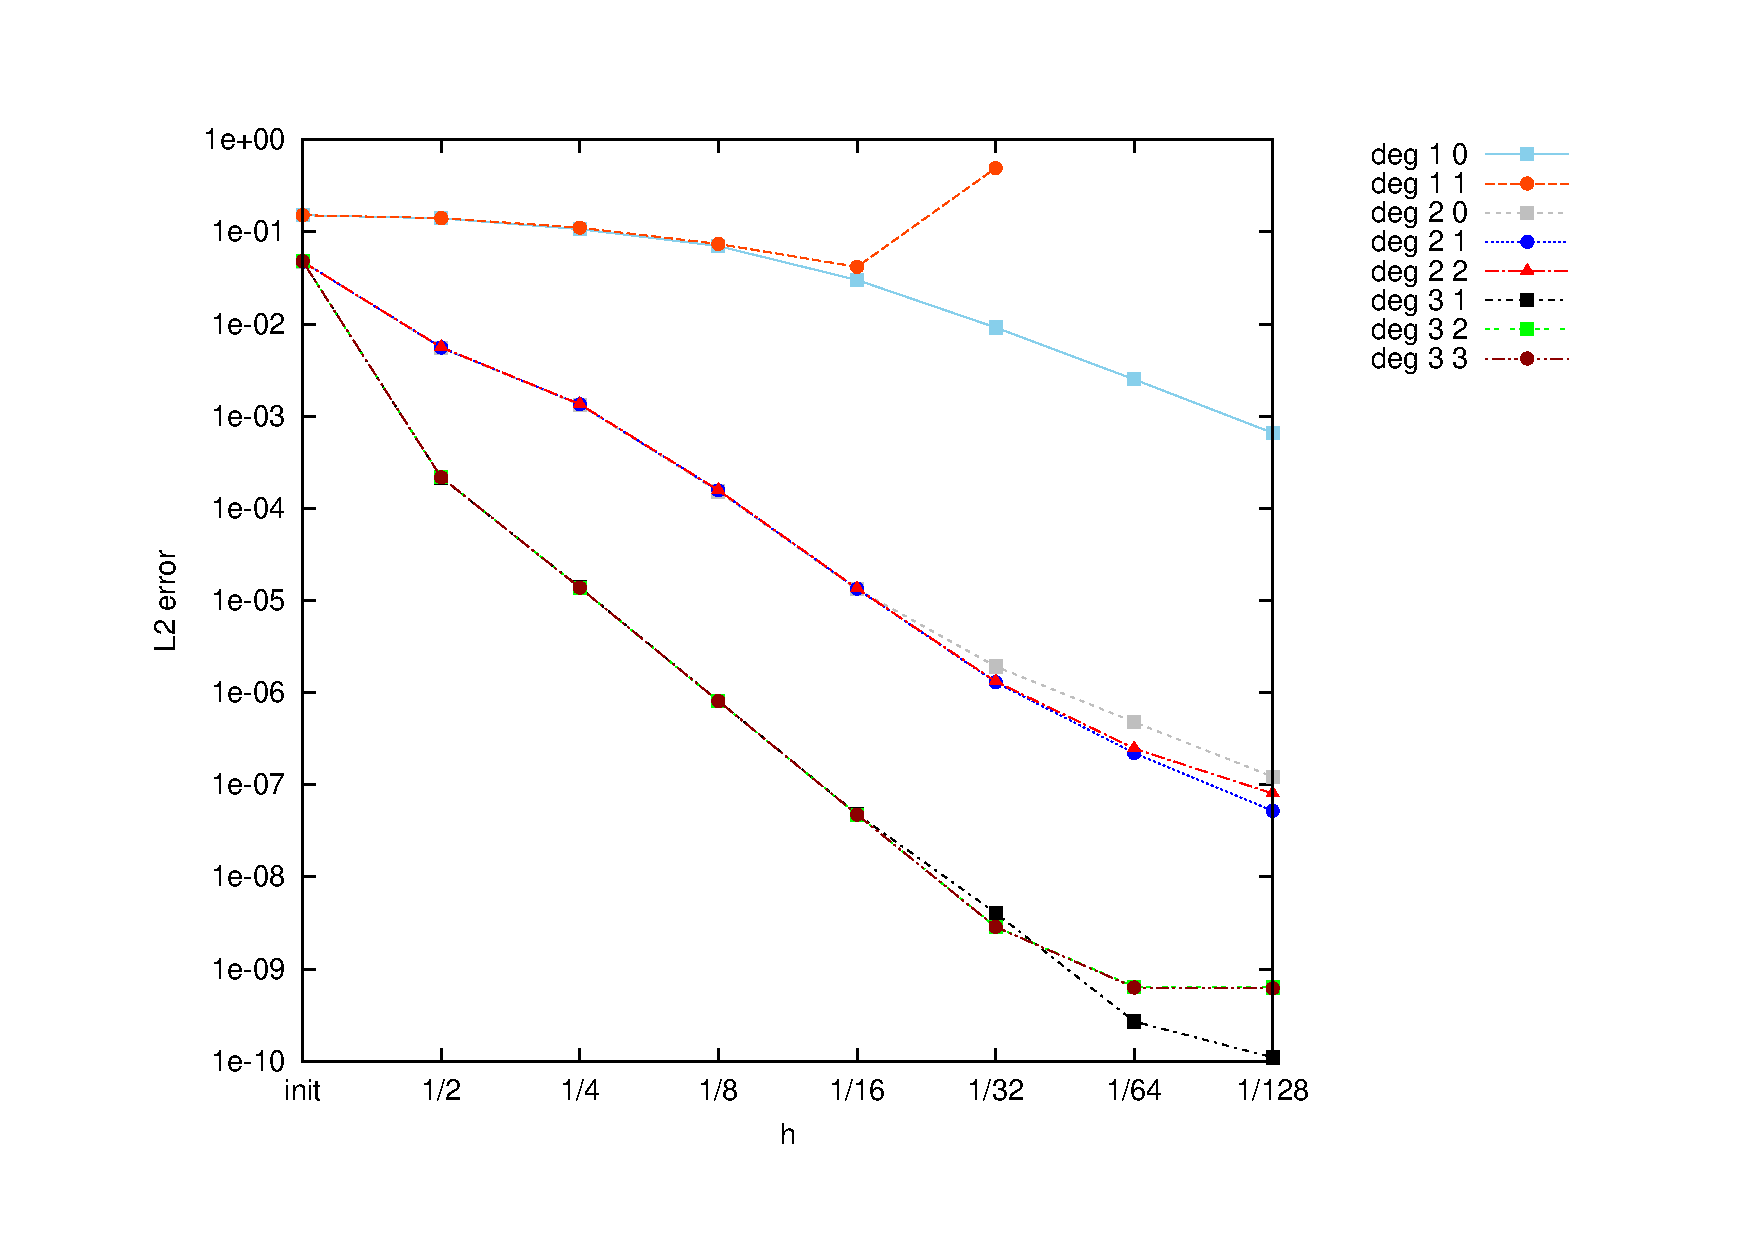
\includegraphics[scale=0.45]{plots/MA1_Neilan_GradJump_l2.pdf}
	\caption{$L^2$ errors for test case \ref{test smooth} and additional gradient jump penalty}
	\label{fig: l2 errors test 1 jump}
\end{figure}
\begin{table}[H]
	\begin{subtable}[b]{0.4\textwidth}
		\centering
		\pgfplotstabletypeset[
		columns={iterations, l2error, h1error,N},
		every row 0 column 0/.style={set content=init},
		]\MAOneJumpdegTwoTwo
		\caption{Error for $k=2, k_{DH}=2$}
	\end{subtable}
	~
	\begin{subtable}[b]{0.4\textwidth}
		\centering
		\pgfplotstabletypeset[columns={iterations, l2error, h1error,N},
		every row 0 column 0/.style={set content=init},
		]\MAOneJumpdegTwoZero
		\caption{Error for $k=2, k_{DH}=0$}
	\end{subtable}
	\caption{Errors for test case \ref{test smooth} with additional jump penalty}
	\label{tab: l2 errors test 1 deg 2 jump}
\end{table}
\begin{table}[h]
	\begin{subtable}[b]{0.45\textwidth}
		\centering
		\pgfplotstabletypeset[
		columns={iterations, l2error, h1error,N},
		every row 0 column 0/.style={set content=init},
		]\MAOneJumpdegThreeThree
		\caption{Error for $k=3, k_{DH}=3$}
	\end{subtable}
	~
	\begin{subtable}[b]{0.45\textwidth}
		\centering
		\pgfplotstabletypeset[columns={iterations, l2error, h1error,N},
		every row 0 column 0/.style={set content=init},
		]\MAOneJumpdegThreeTwo
		\caption{Error for $k=3, k_{DH}=2$}
	\end{subtable}
	\caption{Errors for test case \ref{test smooth} with additional jump penalty}
	\label{tab: l2 errors test 1 deg 3 jump}
\end{table}

\begin{figure}[H]
\centering
	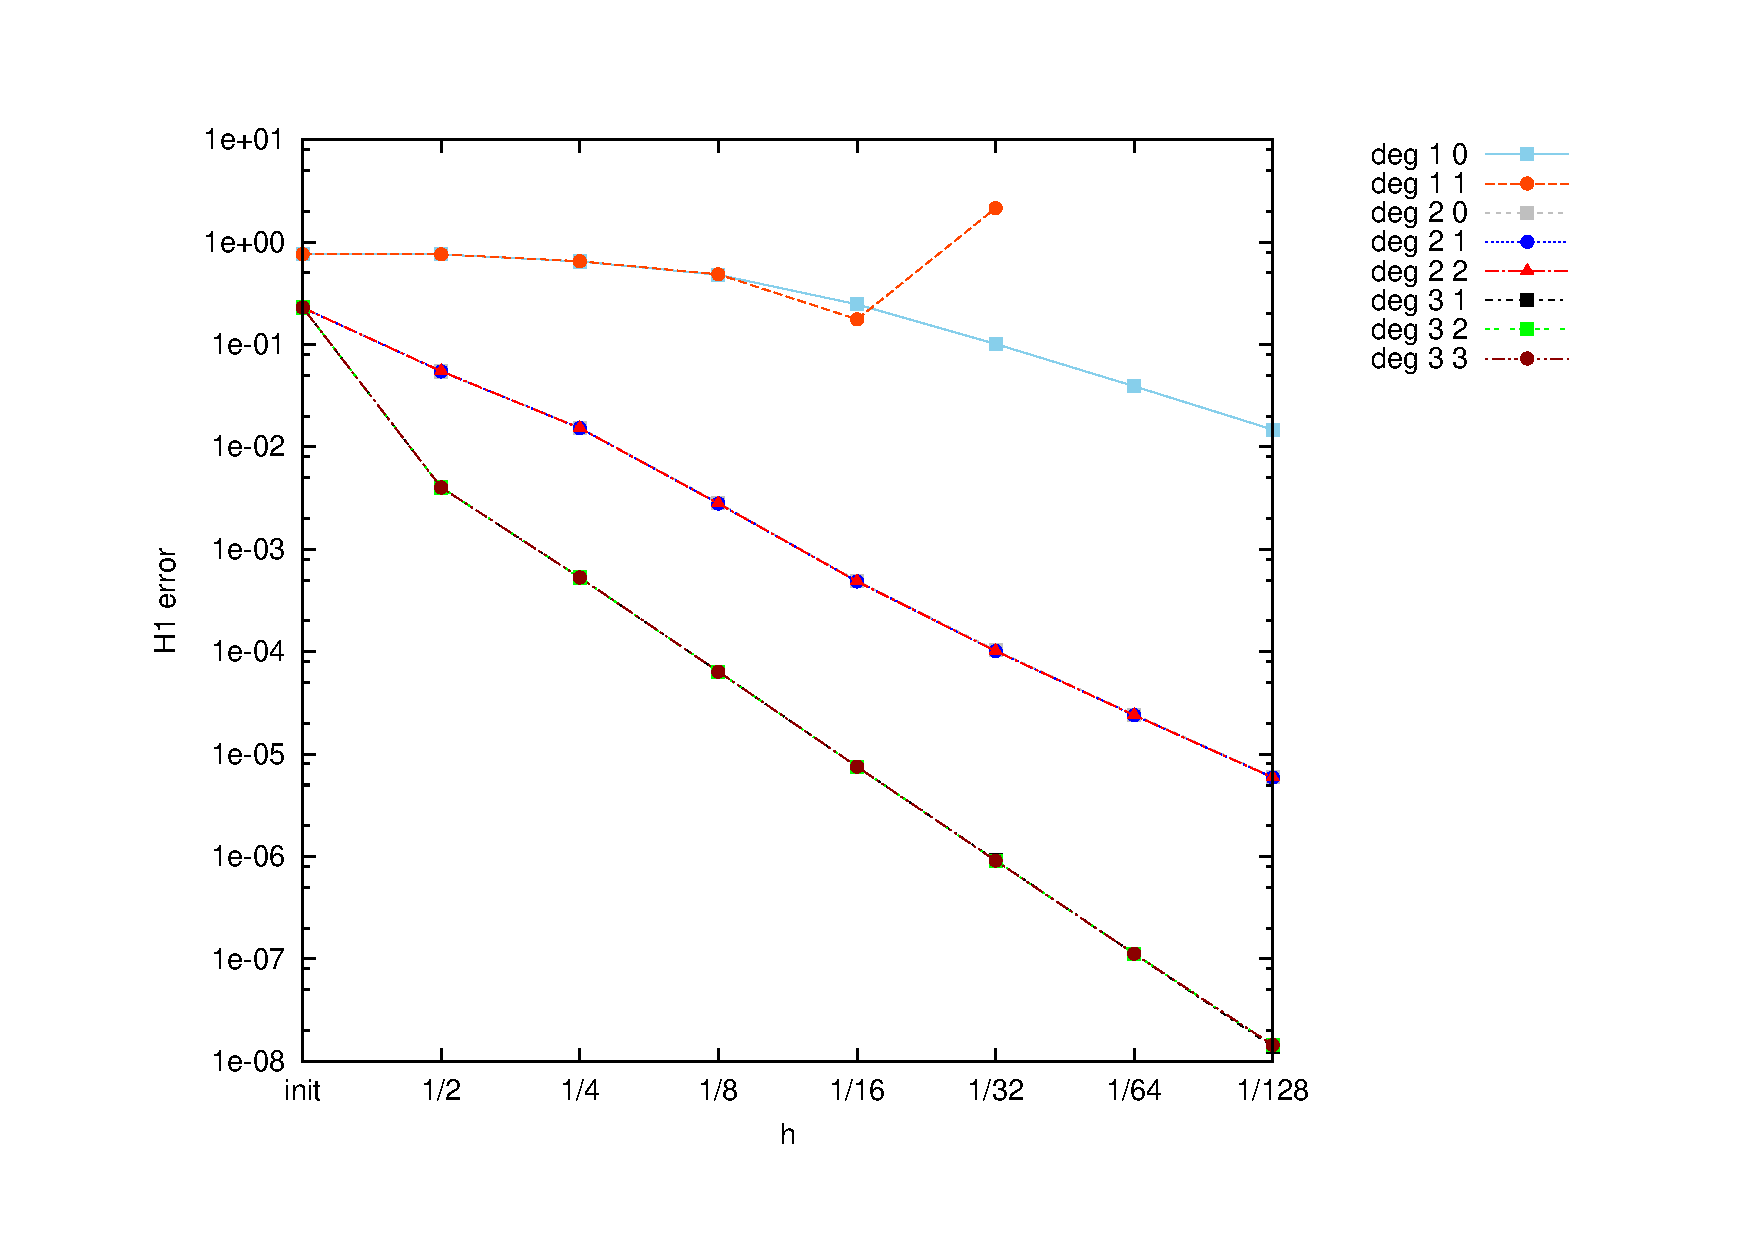
\includegraphics[scale =0.45]{plots/MA1_Neilan_GradJump_h1.pdf}
	\caption{$H^1$ errors for test case \ref{test smooth} and additional gradient jump penalty}
	\label{fig: h1 errors test 1 jump}
\end{figure}

As claimed by Neilan the additional penalisation leads to a convergend method even for low polynomial degrees, even in the cases where only $k_{DH}$ was taken to be small. The only exception is the case $k=1, k_{DH}=1$, for some reason here the method fails. Neilan does not provide any results on this choice of polynomial degrees, he only provides results for $k=1, k_{DH}=0$, $k=2, k_{DH}=2$ and $k=3, k_{DH}=3$. 

Note that the penalised method also for higher degrees performs better than the original ones. This is especially true if $k_{DH}$ was chosen lower than $k$. The numerical orders given in \ref{tab: order jump} confirm this impression and we observe again that the $L^2$ error decreases with order $k+1$ and the $H^1$ error with order $k$. 

Again the calculated error norms indicate that variation of $k_{DH}$ results only in a slight loss of accuracy. For the cases $k=$ and $k_{DH} = 2,3$ the errors and hence, in particular the order, are almost equal. 


\begin{table}[H]
\centering
\begin{subtable}[b]{0.45\textwidth}
	\pgfplotstabletypeset
	{
		k $k_{DH}$ {numerical order}
		1 0 1.32061
		2 0 2.69871
		2 1 2.93488
		2 2 3.0406
		3 1 3.63116
		3 2 4.01895
		3 3 4.0588
	}
	\caption{numerical order in $L2$ norm}
	\end{subtable}
	\begin{subtable}[b]{0.45\textwidth}
	\pgfplotstabletypeset
	{
		k $k_{DH}$ {numerical order}
		1 0 0.978853
		2 0 2.24561
		2 1 2.24836
		2 2 2.28606
		3 1 3.03434
		3 2 3.0359
		3 3  3.0343
	}
	\caption{numerical order in $H1$ norm}
	\end{subtable}
	\caption{numerical order with jump penalty in test \ref{test smooth}}
\label{tab: order jump}
\end{table}


The second test was carried out with the same configuration. Again the size of the system matrices exceeded memory and therefore there are not data points for polynomial degrees $k=2,3$ on fine grids. Table \ref{tab: l2 errors test 2} show the decreasing error norms, it shows only two degree pairs for other degree pairs behaved similarly as we can already see in figure \ref{fig: l2 errors test 2} and \ref{fig: h1 errors test 2}.
\begin{figure}[h]
\centering
	
\includegraphics[scale =0.4]{../../FEniCS/diagrams/MA2_Neilan_l2.pdf}
	\caption{$L^2$ errors for test case \ref{test sqrt} }
	\label{fig: l2 errors test 2}
\end{figure}
\begin{figure}[h]
	\centering
	
\includegraphics[scale =0.4]{../../FEniCS/diagrams/MA2_Neilan_h1.pdf}
	\caption{$H^1$ errors for test case \ref{test sqrt} }
	\label{fig: h1 errors test 2}
\end{figure}
\begin{table}[H]
	\begin{subtable}[b]{0.45\textwidth}
		\centering
		\pgfplotstabletypeset[
		columns={iterations, l2error, h1error,N},
		    every row 0 column 0/.style={set content=init},
		]{\MATwodegTwoTwo}
    	\caption{Error for $k=2, k_{DH}=2$}
   \end{subtable}
   ~
	\begin{subtable}[b]{0.45\textwidth}
		\centering
		\pgfplotstabletypeset[columns={iterations, l2error, h1error,N},
		    every row 0 column 0/.style={set content=init},
		]{\MATwodegThreeThree}
	\caption{Error for $k=3, k_{DH}=3$}
	\end{subtable}
	\caption{Errors for test case \ref{test sqrt}}
	\label{tab: l2 errors test 2}
\end{table}

\begin{table}[H]
\centering
\begin{subtable}[b]{0.45\textwidth}
	\pgfplotstabletypeset
	{
		k $k_{DH}$ {numerical order}
		2 1 1.55213
		2 2 1.63088 
		3 2 1.64644
		3 3 1.64841
	}
	\caption{numerical order in $L2$ norm}
	\end{subtable}
	\begin{subtable}[b]{0.45\textwidth}
	\pgfplotstabletypeset
	{
		k $k_{DH}$ {numerical order}
		2 1 0.465187
		2 2 0.473759
		3 2 0.475829
		3 3  0.495565
	}
	\caption{numerical order in $H1$ norm}
	\end{subtable}
	\caption{numerical order with jump penalty in test \ref{test smooth}}
\label{tab: order jump test 2}
\end{table}

Switching the penalisation of gradient jumps on the method performs again well, its results are shown in figure \ref{fig: l2 errors test 2 jump} and the tables . 
\begin{figure}[H]
\centering
\begin{subfigure}{\textwidth}
\centering
	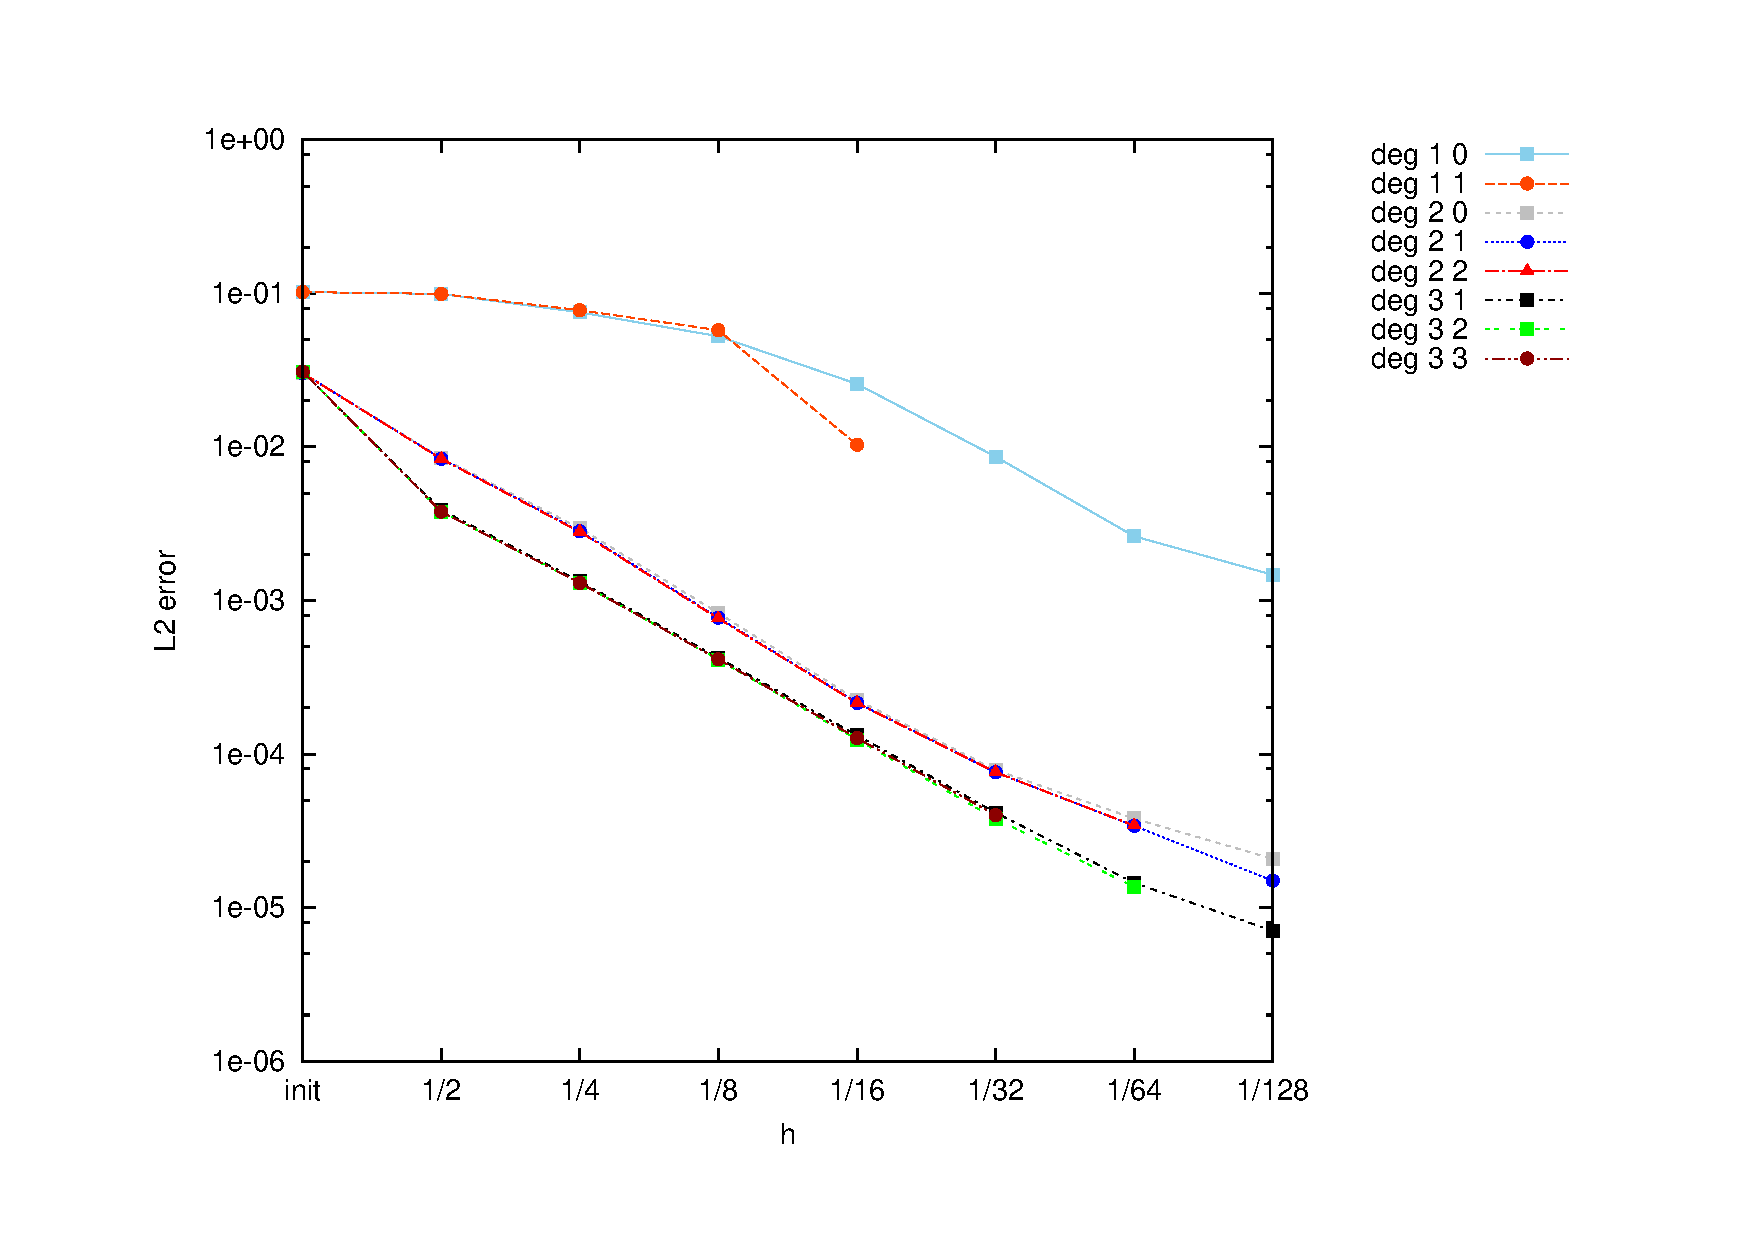
\includegraphics[scale =0.4]{../../FEniCS/diagrams/MA2_Neilan_GradJump_l2.pdf}
\end{subfigure}

\begin{subfigure}{\textwidth}
\centering
	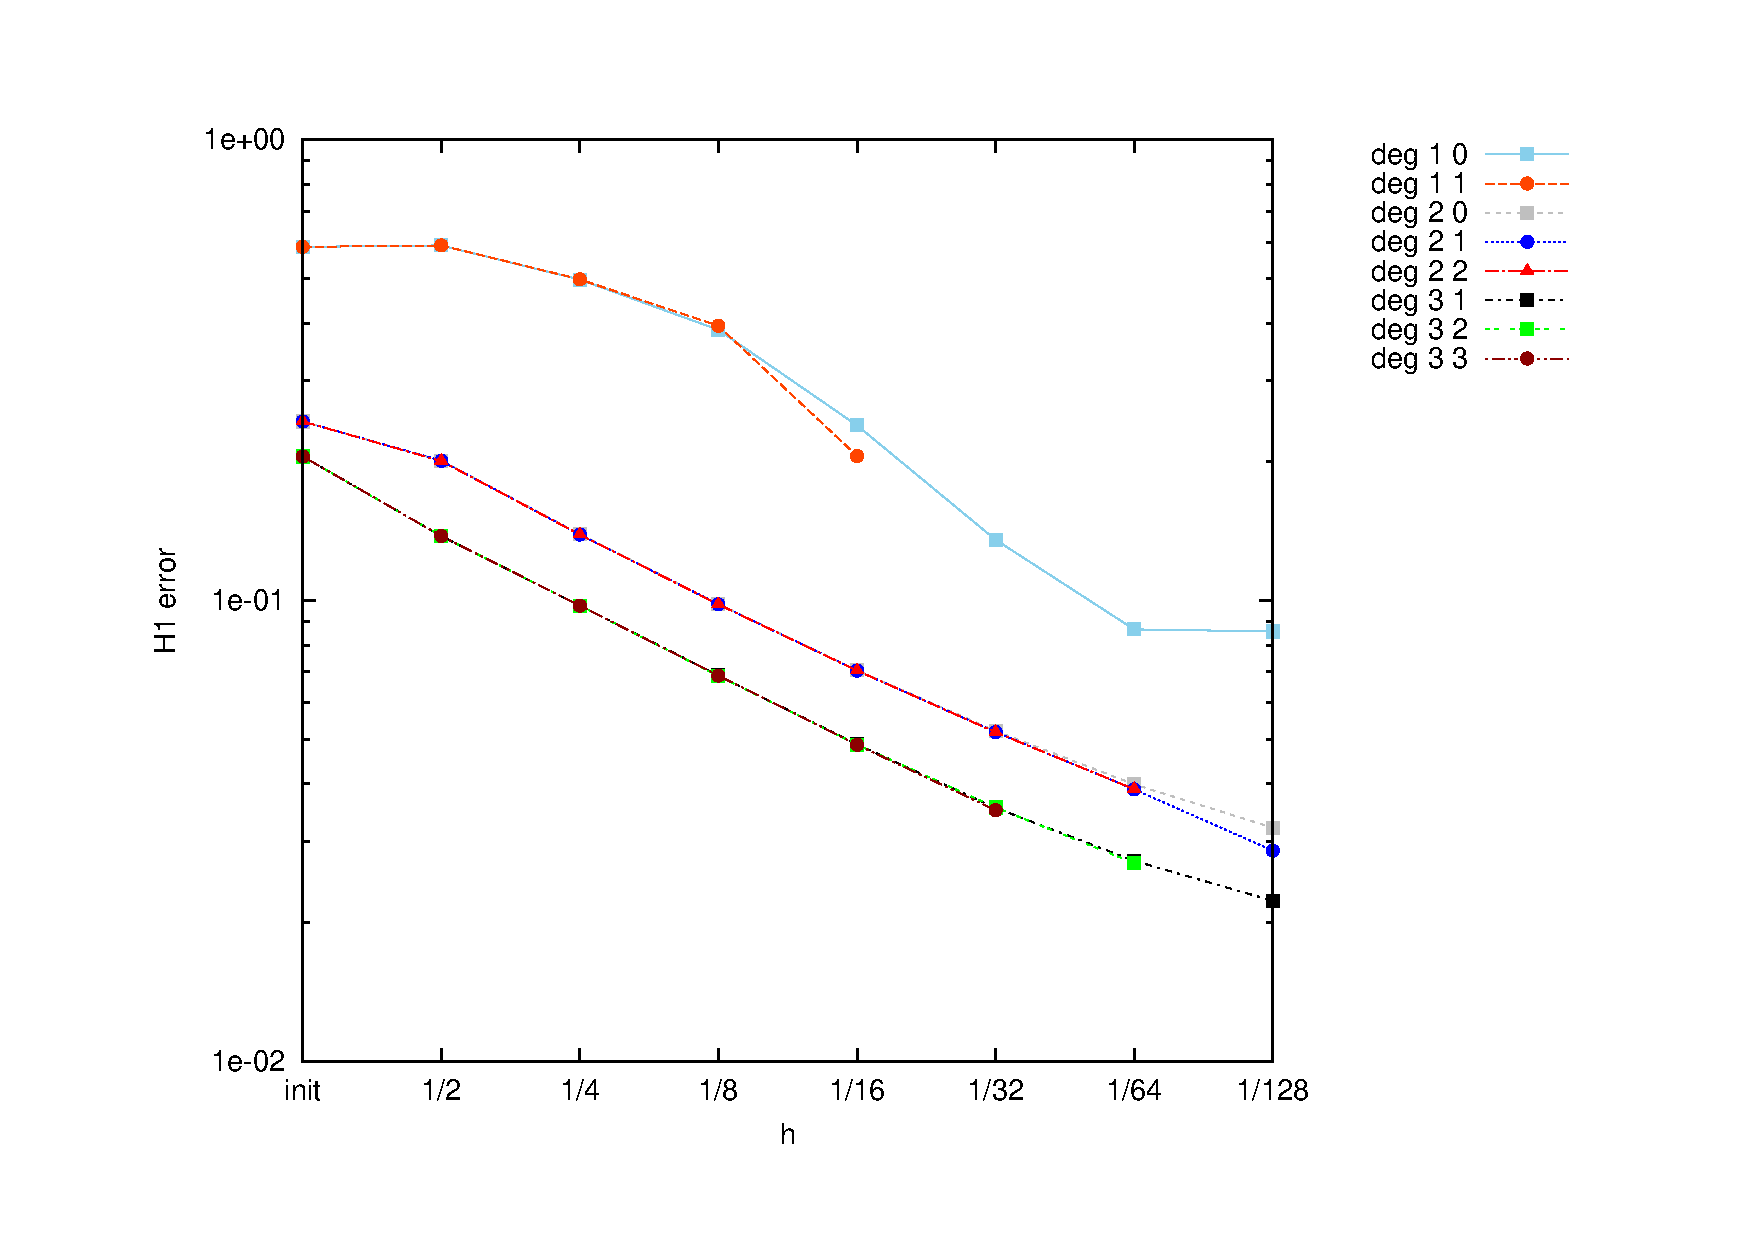
\includegraphics[scale =0.4]{../../FEniCS/diagrams/MA2_Neilan_GradJump_h1.pdf}
\end{subfigure}
	\caption{$L^2$ and $H^1$ errors for test case \ref{test sqrt} and additional gradient jump penalty}
	\label{fig: l2 errors test 2 jump}
\end{figure}
\begin{table}[H]
	\begin{subtable}[b]{0.45\textwidth}
		\centering
		\pgfplotstabletypeset[
		columns={iterations, l2error, h1error,N},
		every row 0 column 0/.style={set content=init},
		]{\MATwoJumpdegTwoTwo}
		\caption{Error for $k=2, k_{DH}=2$}
	\end{subtable}
	~
	\begin{subtable}[b]{0.45\textwidth}
		\centering
		\pgfplotstabletypeset[columns={iterations, l2error, h1error,N},
		every row 0 column 0/.style={set content=init},
		]{\MATwoJumpdegThreeThree}
		\caption{Error for $k=3, k_{DH}=3$}
	\end{subtable}
	\caption{Errors for test case \ref{test sqrt} with additional }
	\label{tab: l2 errors test 2 jump}
\end{table}

As we can see the results do not alter between the method with or without additional penalty on the gradient. Therefore also the numerical orders are almost identical.  
%\begin{table}[H]
%\centering
%\begin{subtable}[b]{0.45\textwidth}
%	\pgfplotstabletypeset
%	{
%		k $k_{DH}$ {numerical order}
%		1 0 1.03719 
%		2 1 1.55213
%		2 2 
%		3 2 
%		3 3 
%	}
%	\caption{numerical order in $L2$ norm}
%	\end{subtable}
%	\begin{subtable}[b]{0.45\textwidth}
%	\pgfplotstabletypeset
%	{
%		k $k_{DH}$ {numerical order}
%		2 1 
%		2 2 
%		3 2 
%		3 3  
%	}
%	\caption{numerical order in $H1$ norm}
%	\end{subtable}
%	\caption{numerical order with jump penalty in test \ref{test smooth}}
%\label{tab: order jump test 2}
%\end{table}


Similar are results for Test \ref{test singularity}, also a problem without a classical solution. Without additional gradient penalty the method does not work well as could be seen in Table \ref{tab: l2 errors test 3} where all converged iteration steps for polynomial degree $k=2, k_{DH}=2$ are shown.
\begin{table}[H]
%	\begin{subtable}[b]{0.45\textwidth}
		\centering
		\pgfplotstabletypeset[
		columns={iterations, l2error, h1error,N},
		    every row 0 column 0/.style={set content=init},
		]{\MAThreedegTwoTwo}
%   \end{subtable}
%   ~
%	\begin{subtable}[b]{0.45\textwidth}
%		\centering
%%		\pgfplotstabletypeset[columns={iterations, l2error, h1error,N},
%%		    every row 0 column 0/.style={set content=init},
%%		]{\MAThreedegThreeThree}
%	\caption{Error for $k=3, k_{DH}=3$}
%	\end{subtable}
	\caption{Errors for Test \ref{test singularity} for $k=2, k_{DH}=2$}
	\label{tab: l2 errors test 3}
\end{table}

The results of the corresponding method with additional jump penalisation can be found in Figure \ref{fig: l2 errors test 3 jump} and Figure \ref{fig: h1 errors test 3 jump}, as well as in Table \ref{tab: l2 errors test 3 jump}. 

As in Test \ref{test smooth} the pair $k=1$ and $k_{DH}=1$ induces a unstable method. We further observe that the method with $k=2$ performs well on coarse grids, whereas for $k=3$ Newton's method does not converge on the coarsest grid. 

The numerical orders given in Table \ref{tab: order jump 3} show the error decreases faster for quadratic polynomials during the first refinements. Yet, for grids with $h \geq \frac 1 {32}$ only the pairing $k=1$ and $k_{DH} =0$ yields to convergence.

\begin{figure}[H]
	\centering
	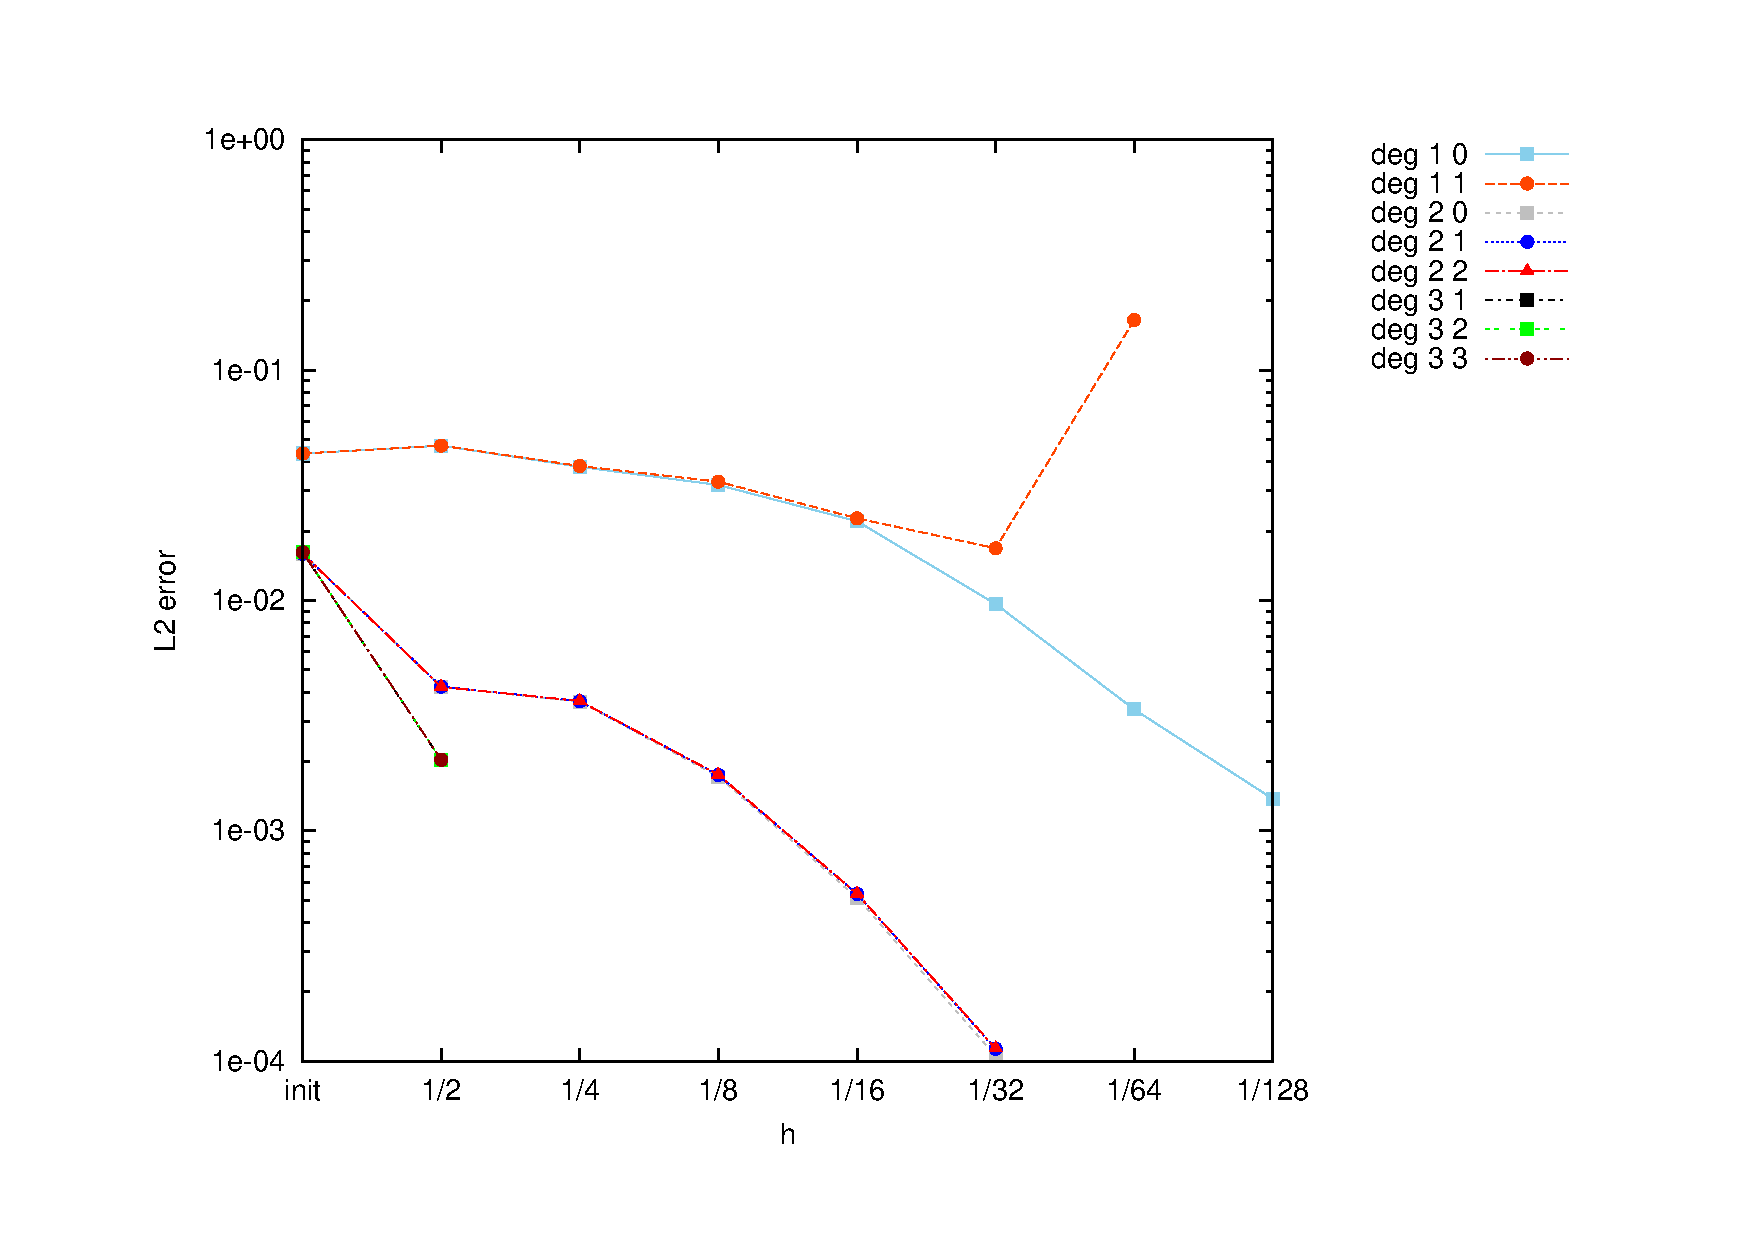
\includegraphics[scale =0.45]{plots/MA3_Neilan_GradJump_l2.pdf}
	\caption{$L^2$ errors for Test \ref{test singularity} and additional gradient jump penalty}
	\label{fig: l2 errors test 3 jump}
\end{figure}

\begin{figure}[H]
	\centering
	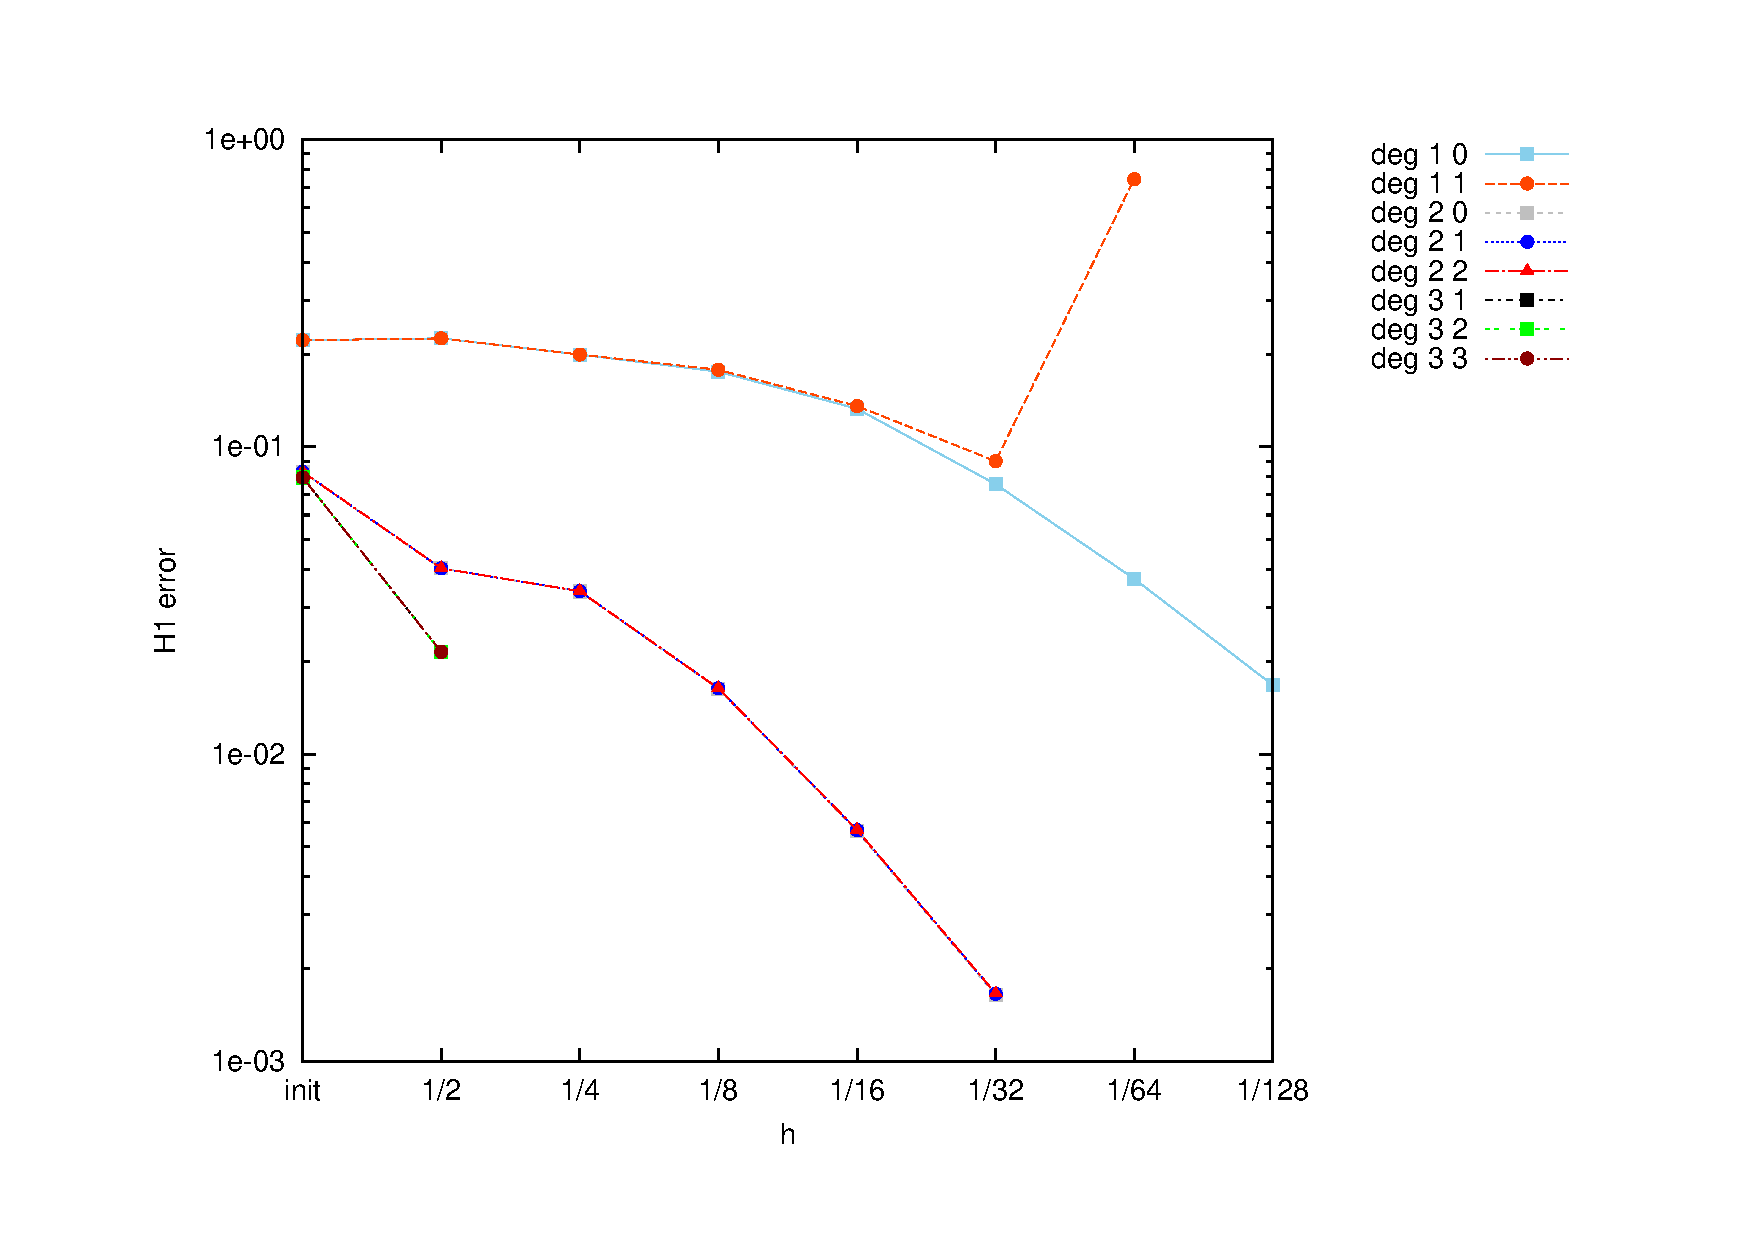
\includegraphics[scale =0.4]{plots/MA3_Neilan_GradJump_h1.pdf}
	\caption{$H^1$ errors for Test \ref{test singularity} and additional gradient jump penalty}
	\label{fig: h1 errors test 3 jump}
\end{figure}

\begin{table}[h]
	\begin{subtable}[b]{0.45\textwidth}
		\centering
		\pgfplotstabletypeset[columns={iterations, l2error, h1error,N},
		every row 0 column 0/.style={set content=init},
		]{\MAThreeJumpdegOneZero}
		\caption{Error for $k=1, k_{DH}=0$}
	\end{subtable}
	~
	\begin{subtable}[b]{0.45\textwidth}
		\centering
		\pgfplotstabletypeset[
		columns={iterations, l2error, h1error,N},
		every row 0 column 0/.style={set content=init},
		every row 6 column 1/.style={set content=-},
		every row 6 column 2/.style={set content=-},
		every row 6 column 3/.style={set content=-},
		every row 7 column 1/.style={set content=-},
		every row 7 column 2/.style={set content=-},
		every row 7 column 3/.style={set content=-},
		]{\MAThreeJumpdegTwoTwo}
		\caption{Error for $k=2, k_{DH}=2$}
	\end{subtable}
	\caption{Errors for Test \ref{test singularity} and additional gradient jump penalty}
	\label{tab: l2 errors test 3 jump}
\end{table}	

\begin{table}[H]
\centering
\begin{subtable}[b]{0.45\textwidth}
	\pgfplotstabletypeset
	{
		k $k_{DH}$ {numerical order}
		1 0 0.8565
		2 1 1.32222
		2 2 1.32048
	}
	\caption{numerical order in $L2$ norm}
	\end{subtable}
	\begin{subtable}[b]{0.45\textwidth}
	\pgfplotstabletypeset
	{
		k $k_{DH}$ {numerical order}
		1 0 0.618481
		2 1 1.17823
		2 2 1.17823
	}
	\caption{numerical order in $H1$ norm}
	\end{subtable}
	\caption{Numerical order with jump penalty in Test \ref{test singularity}}
\label{tab: order jump 3}
\end{table}




For the last test case the method without additional gradient jump were did not work out just as in the previous test cases. We therefore only concentrate on the performances penalising the normal gradient jump across edges. The error made is to be found in the plots in Figures \ref{fig: l2 errors test 3 jump} \ref{fig: h1 errors test 3 jump}, as wells as in Table \ref{tab: l2 errors test 4 jump}. Again Newton's method did not converge for $k=2,3$ on fine grids. 
\begin{table}[H]
	\begin{subtable}[b]{0.45\textwidth}
		\centering
		\pgfplotstabletypeset[columns={iterations, l2error, h1error,N},
		every row 0 column 0/.style={set content=init},
		]{\MAFourJumpdegOneZero}
		\caption{Error for $k=1, k_{DH}=0$}
	\end{subtable}
	~
	\begin{subtable}[b]{0.45\textwidth}
		\centering
		\pgfplotstabletypeset[
		columns={iterations, l2error, h1error,N},
		every row 0 column 0/.style={set content=init},
		every row 5 column 1/.style={set content=-},
		every row 5 column 2/.style={set content=-},
		every row 5 column 3/.style={set content=-},
		every row 6 column 1/.style={set content=-},
		every row 6 column 2/.style={set content=-},
		every row 6 column 3/.style={set content=-},
		every row 7 column 1/.style={set content=-},
		every row 7 column 2/.style={set content=-},
		every row 7 column 3/.style={set content=-},
		]{\MAFourJumpdegTwoTwo}
		\caption{Error for $k=2, k_{DH}=2$}
	\end{subtable}
	\caption{Errors for test case \ref{test dirac} and additional gradient jump penalty}
	\label{tab: l2 errors test 4 jump}
\end{table}


\begin{figure}[H]
	\centering
		\centering
		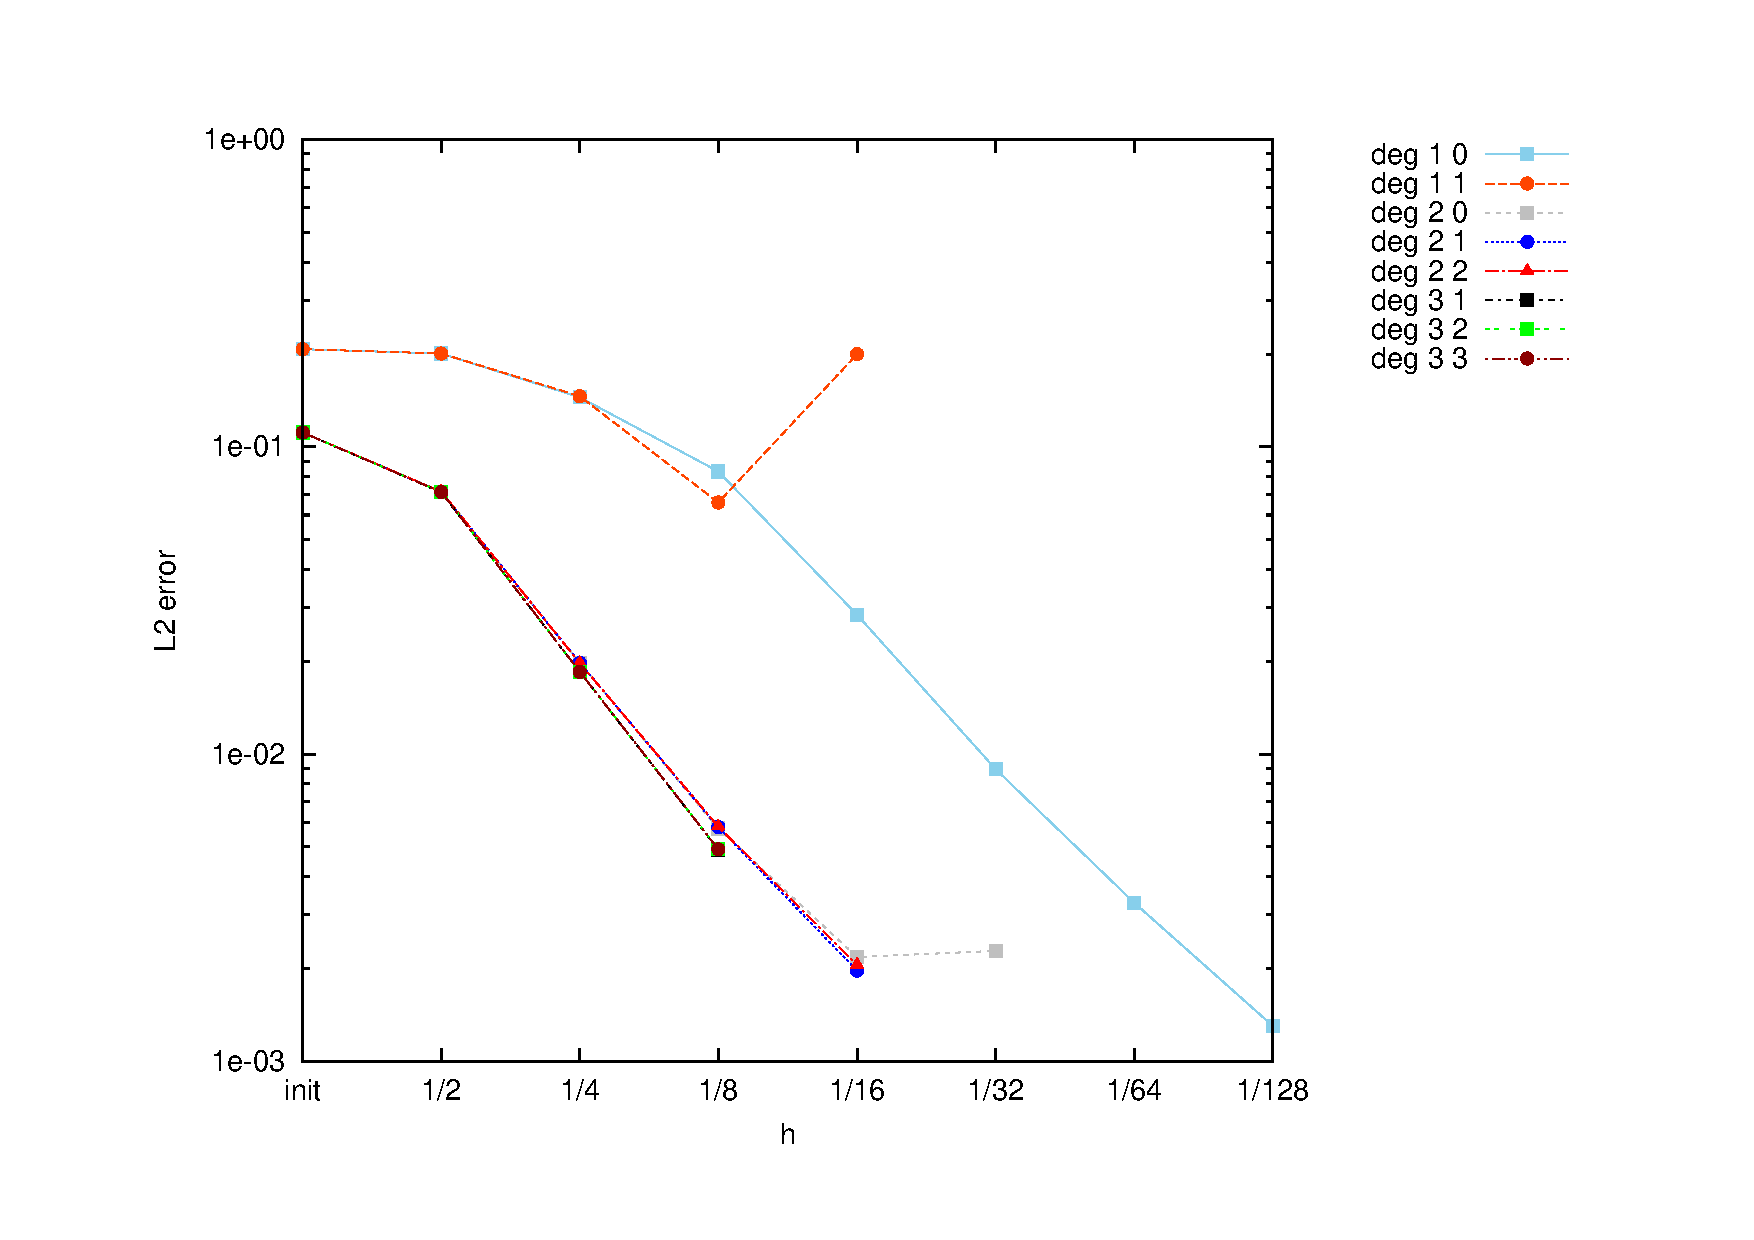
\includegraphics[scale =0.4]{plots/MA4_Neilan_GradJump_l2.pdf}
	\caption{$L^2$ errors for test case \ref{test dirac} and additional gradient jump penalty}
	\label{fig: l2 errors test 4 jump}
\end{figure}
	
\begin{figure}[H]
		\centering
		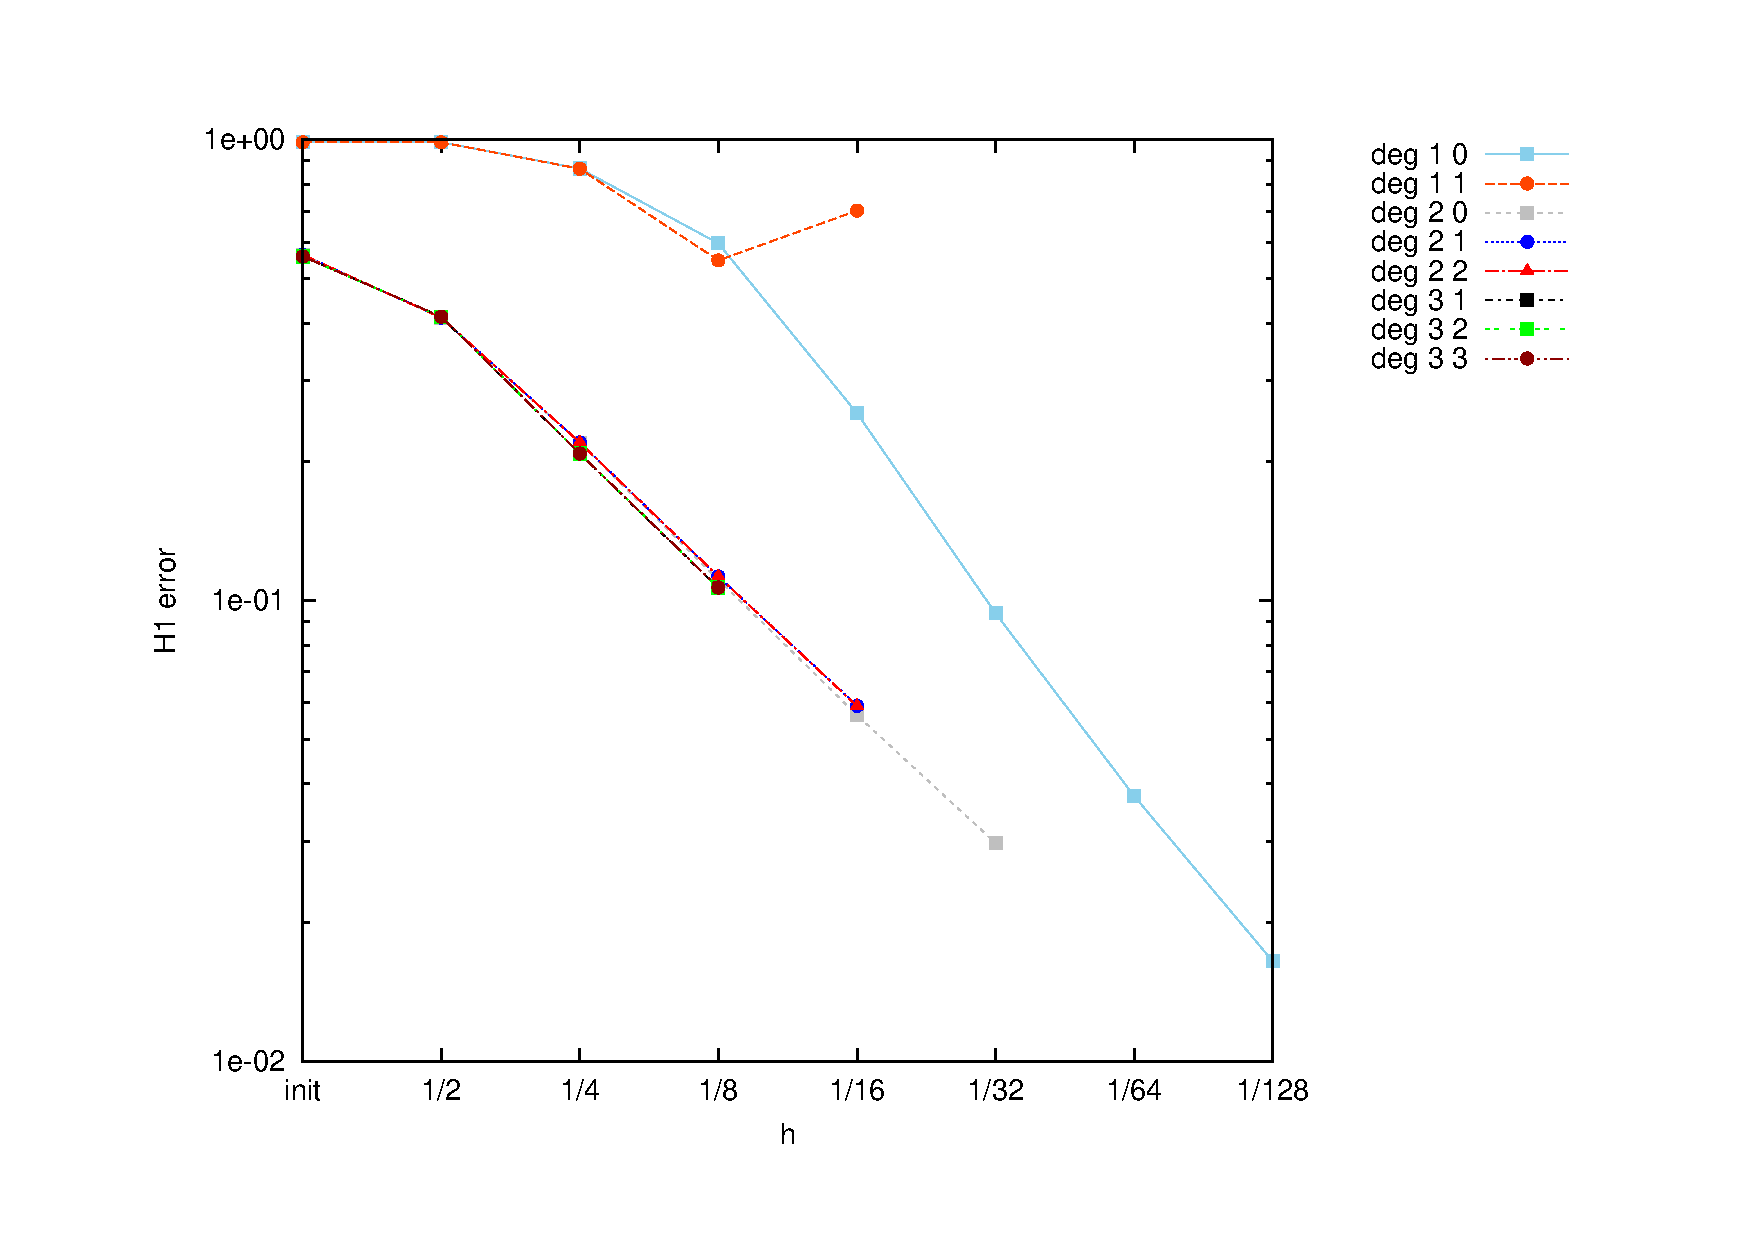
\includegraphics[scale =0.4]{plots/MA4_Neilan_GradJump_h1.pdf}
	\caption{$H^1$ errors for test case \ref{test dirac} and additional gradient jump penalty}
	\label{fig: h1 errors test 4 jump}
\end{figure}
As before we do not observe much difference between the choices $k=2$ and $k=3$ during the first (converged) refinements. But as the Aleksandrov solution of this test case lacks regularity it is not surprising that increasing the polynomial degree does not effect the error.

It is noticeable that for $k=2$ the $L^2$ error increases after four refinement while the $H^1$ error decreases, we already experienced this behaviour in test \ref{test smooth}.

%\todo{symmetrised neilan and not crossed grid}

\newpage

\section{Numerical Results of DG Picard Iteration Method}

The Picard iteration is implemented in C++. All vector and matrix handling as well as was linear solvers are provided by the Eigen library \cite{eigenweb}. To solve the quadratic program arising in the context of a convexification (cf. \eqref{eq: convex lsq}) the C++ library ipopt \cite{ipopt} was used.

The C++ implementation uses the same nested grids as also have been used in the latter FEniCS implementations (cf. Figure \ref{fig: grids}). It is obtained by dividing the unitsquare along the diagonals into four triangles and then refining uniformly as explained in \ref{subsec: refinement and base cells}.

\subsection{Implementation Details}

The main class of the implementation is the Tsolver class. The solver collects all information and controls the assembly and solving process.
Hence, the main method which can be found in mesh.cpp just initialises solver and starts the solving process: Via a configuration file all input data is fed into the main routine. With this information the solver can initialise its members grid and Tshape, Those represent the underlying grid structure and the reference cell. 
The grid implemenation is taken from the igpm\_t2\_lib and is based on the work of \cite{BMV2009}.

The main method, i.e. the algorithm from Algorithm \ref{alg: final} is implemented in Tsolver's function stepping\_MA(). It starts with an initialisation process where it reads specific problem data which includes
\begin{enumerate}
 \item the problem we want to solve,
 \item penalty parameters to enforce continuity and penalise the gradient jump,
 \item the start level of refinement with respect to the initial grid $start\_level$,
 \item the damping paramter $\alpha$,
 \item the number of fixed point iterations per grid $max\_its$,
 \item the maximal grid refinements $max\_levelrefinement$.
\end{enumerate}
During the initialisation the methods also updates all base cell data and leaf cell data, enumerates the degree of freedoms and computes the initial guess.\\
Afterwards the fixed point iterations begins, in every step the General Poisson problem (cf. Section \ref{sec: SIPG MA}) solved, eventually convexified (cf. Section \ref{subsec: convexification}) and afterwards with the last solution step combined \ref{subsec: add penalty param}). If the specified number of iterations has been carried out, the grid is refined, the leaf cell data updated and we start the fixed point iterations again.
We repeat this process until the maximal number of grid refinements is reached.
To illustrate this procedure Algorithm \ref{alg: stepping} shows the function stepping\_MA() in pseudo code.
\begin{algorithm}[H]
\begin{algorithmic}
	\State Read problem specific data
%		\begin{enumerate}
%			 \item  problem\_name \Comment {to choose right-hand side and boundary conditions}
%			 \item penalty parameters   \Comment {  to enforce continuity and penalise the gradient jump}
%			 \item start\_level  \Comment { the start level of refinement with respect to the input grid}
%			 \item $\alpha$  \Comment {the damping paramter}
%			 \item maxits \Comment{ the number of fixed point iterations per grid}
%			 \item max\_levelrefinement \Comment{ the maximal refinement level }
%		\end{enumerate}
	\State Initialise base cell data
	\State Refine to $start\_level$
	\State Initialise leaf cell data
	\State Enumerate degree of freedoms
	\State (Initialise Convexifier)
	\State Initialise initial guess $u_{-1}$
	\State level $\gets start\_level$
	\State $i \gets 0$
	\While {level < $max\_levelrefinement$}
		\State Enumerate degree of freedoms
		\State Update base and leaf cell data
		\State (Initialise C0 converter) \Comment{only needed for convexification}
		\State cur\_it$ \gets 0$
		\While {cur\_it < $maxits$}
			\State  assemble\_MA()                              \Comment Assemble system for General Poisson problem
			\State $u_i \gets$ solution of assembled system
			\State (Convexify $u_i$)		 
			\State $u_i \gets \alpha u_{i-1}  +(1-\alpha) u_i$
			\State	cur\_it, i $\gets$ cur\_it$+1$, i$+1$
			\State Restore\_MA() 		\Comment{Store solution in leaf cells}
		\EndWhile
		\State Refine grid and update leaf cell data
		\State level $\gets$ level $+1$
	\EndWhile
\end{algorithmic}
\caption{stepping\_MA}
\label{alg: stepping}
\end{algorithm}

After we have seen the program structure I shortly remark some of arising programming issues:

Before the actual system assembly the diffusion matrix in every cell has to be updated with the modified cofactor matrix of the Hessian of the last Picard step. Note that this matrix is constant for polynomial degree $k=2$ and otherwise has to be calculated at every quadrature point. Since in general here is no connection between diffusion matrix values at the reference cell and in the leaf cell, we cannot save easily any memory as we did for function values and normal gradients (cf. Section \ref{subsec: ref cell} and \ref{subsec: refinement and base cells}). Hence, we store the diffusion matrix at every quadrature point on the grid in the corresponding leaf cell.
The rest of the assembly process is carried out as already mentioned in algorithm \ref{alg: assembling}. Hereby one has to pay attention to the right scaling of quadrature weights and the right calculation of quadrature data from reference cell data as described in Examples \ref{ex: base cell trafo} and \ref{ex: leaf cell trafo}. 

If a convexification is desired, the class Convexifier takes care of the execution of the method described in Section \ref{subsec: convexification}. The linear constraints ensuring convexity on a triangle are chosen to be the ones from theorem \ref{thm: convex cond on triangle} and the constrains for convexity across edges are given by theorem \ref{thm: convex cond across edge}. Due to the error-proneness during the assembly of the constraint matrix $C$ the convexification is only implemented for the case $k=2$. \\
Note that before applying the theorems we have to convert our numerical solution from the DG formulation to a $C^0$ spline.
Hence, at first the Convexifier computes the $C^0$ spline representation of the Poisson solution using the C0converter, and then assembles the matrices $A$ and $C$ of \eqref{eq: convex lsq}. To solve this quadratic problem it makes use of the open source library ipopt \cite{ipopt}.\\
Fortunately the evaluation matrix $A$, and the constraint matrix $C$ of \eqref{eq: convex lsq} only depend on the grid and thus, need only to be computed once in every refinement.

Additionally the Tsolver has a member Plotter handling all export to external files. It is able to write the solution which's coefficients are currently stored in the leaf cells to a .vtu file or .dat file. Besides plotting it also administers all file streams to which information such as $L^2$ errors are written into.

\subsection{Results with Convexification}

For a initial guess I also use the solution of $\triangle u = -\sqrt{2f}$ combined with the nested iteration approach as described in \ref{sec: initial guess}. The grid is chosen as in previous FEniCS implementations to be a refinement of a crisscrossed unit square (cf. Section \ref{sec: numerical results brenner}).
The arising linear system of equations is solved with Eigen's internal Cholesky solver.
The parameters are if not other specified taken to be $\sigma=20 k^2, \sigma_G = 50, \alpha =
0.3$ and $\varepsilon = 1e-2$. We always carry out 15 steps including a convexification after every step before we refine further.
\begin{figure}[H]
\centering
	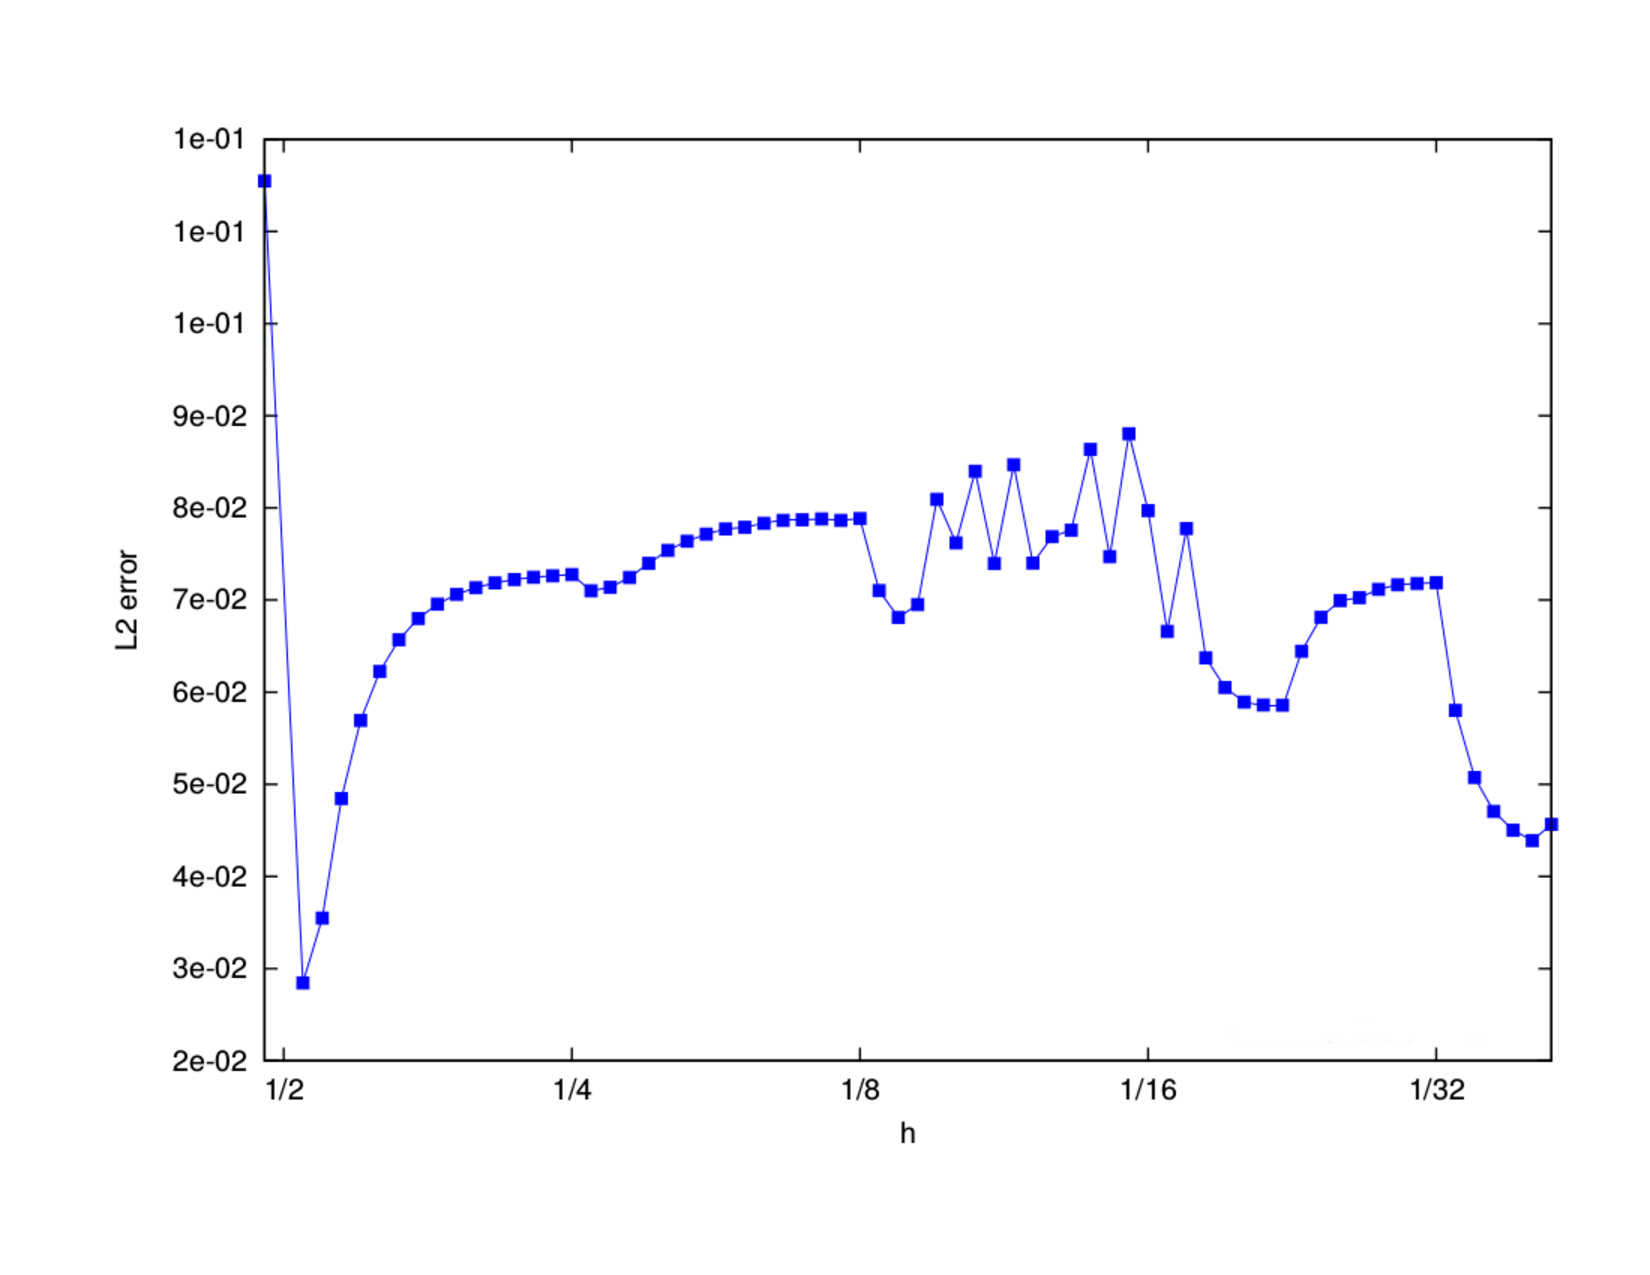
\includegraphics[scale =0.4]{plots/MA1_convexify.pdf}
	\caption{$L^2$ errors for test case \ref{test smooth} and additional convexification}
	\label{fig: l2 errors test smooth ourMethodConvex}
\end{figure}
The implemented convexification follows the ideas of Section \ref{subsec: convexification}. \\
The plots given in Figure \ref{fig: l2 errors test smooth ourMethodConvex} show the $L^2$ error of $u_i$ obtained by the calculations as described in Section \ref{sec: Picard Iteration Algo}. We recall that means $u_i$ is obtained by combining the old step with a convexified Poisson solution. Unfortunately, the method with the convexification process does not work as expected.
To investigate this failure we give in Figure \ref{fig: convex before after} the plot of the $L^2$ error before the convexification step and the plot after it. As we can see the convexification process increases the error. There are several possible explanations for that:

Though the convexification algorithm produces a convex result it does not garantuee that it leaves convex input functions unchanged.

The convex function in the space of piecewise polynomials $\mathcal P^2_h$ approximating the numerical solution $u_h$ best is not necessarily closer to the exact solution $u$ than $u_h$. %Then the convexification gives a push into the wrong direction.

The best approximation of $u$ into $\mathcal P^2_h$ does not have to be convex, for example the affine Lagrange interpolant of a convex function does not to be convex\cite[p.3142]{AM2009}. 

To understand how \quoting{unconvex} the function was before the convexification process I have examined the vector $Cc_u$ where $C$ is the matrix containing the convexity conditions and $c_u$ are the coefficients of $L^2$ projection into $\mathcal P^2_h$ (cf. \eqref{eq: convex lsq}): The minimal entry for a grid with $h=1/2$ is -9.77e-03, for a grid with $h=1/16$ the minimal entry is -4.26e-04. Thus, the $L2$ projection of the exact solution does not comply with the convexity conditions.
Figure \ref{fig: convex min coeffs} plots the minimal entry of $Cc$ during the Picard iterations, where $c$ are the B\'ezier coefficients of the Poisson solutions. We see that especially for small grid widths the Poisson solutions do not fulfill the convexity conditions. 

\begin{figure}[H]
\centering
	\begin{subfigure}{0.45\textwidth}
		\centering
		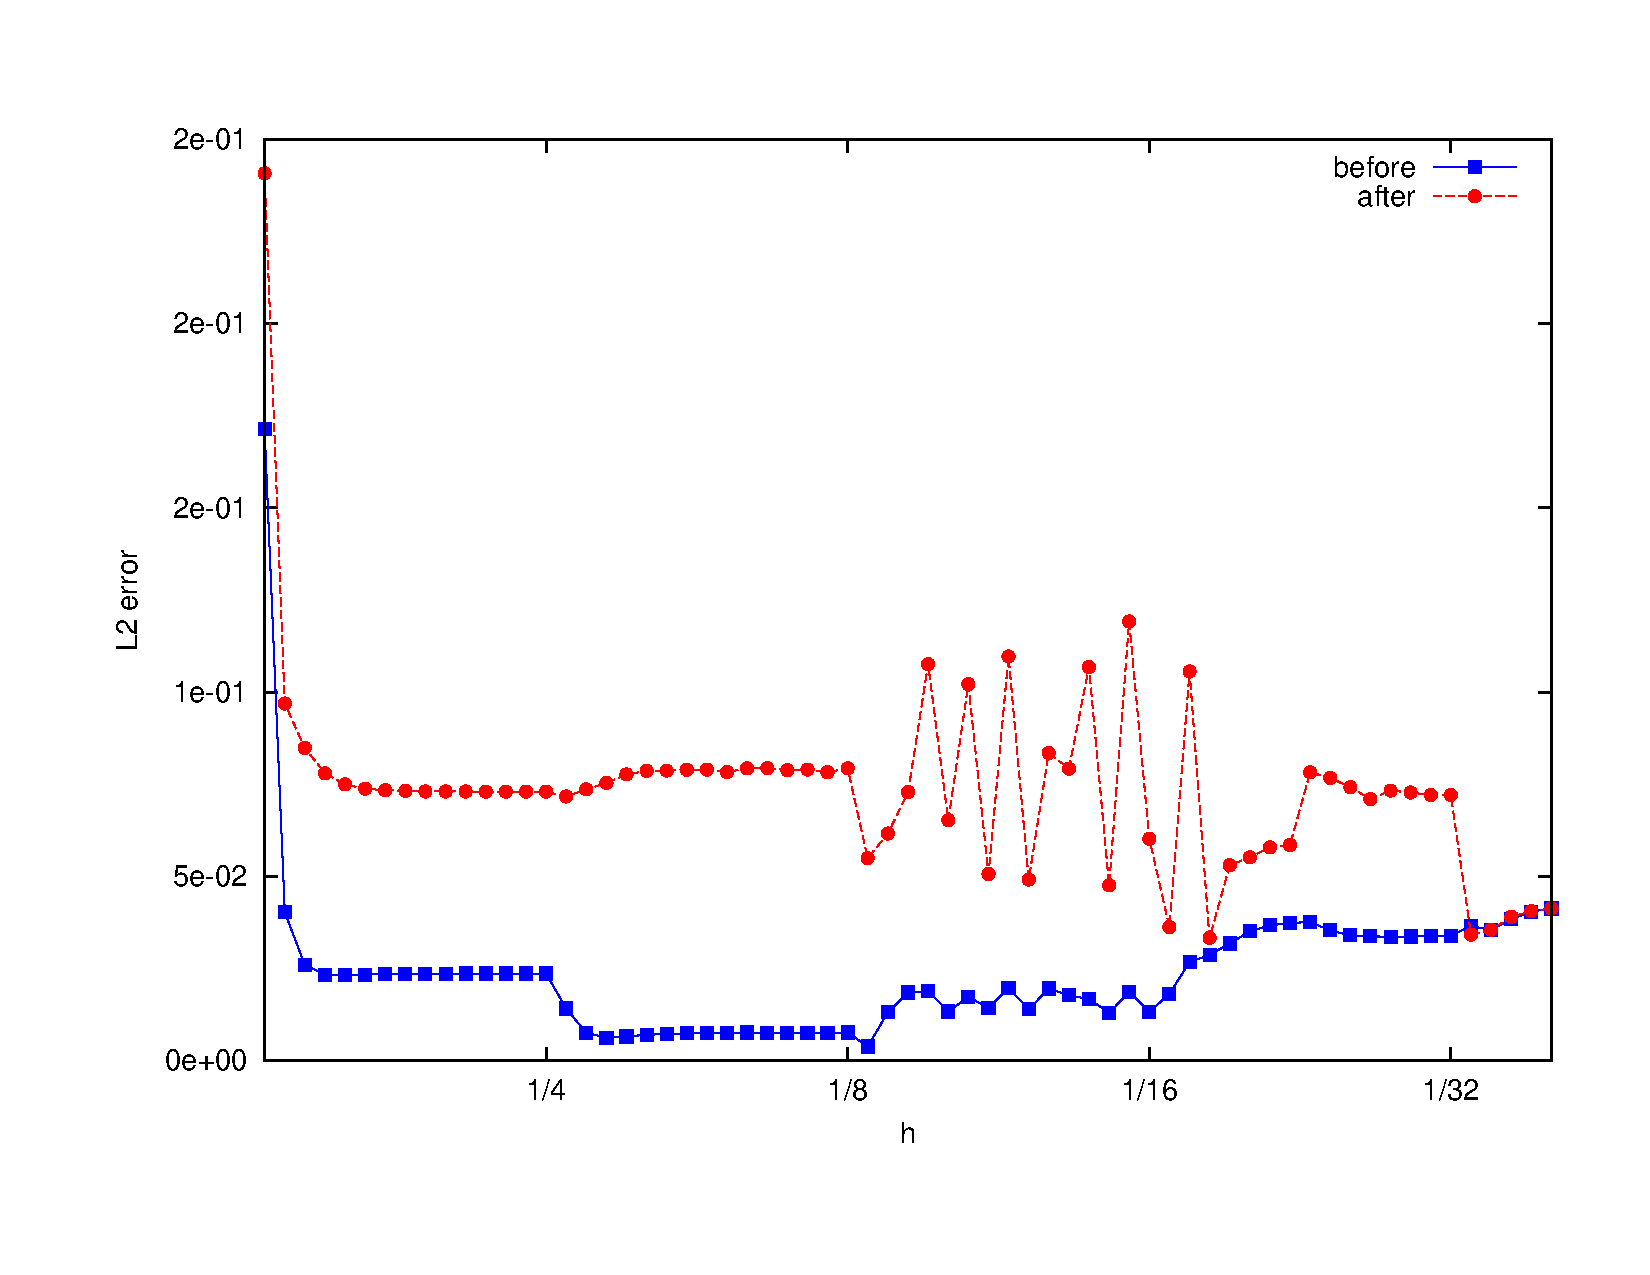
\includegraphics[scale=0.25]{plots/MA1_convexComp.pdf}
		\caption{Comparison of $L^2$ errors directly before and after convexification}
		\label{fig: convex before after}
	\end{subfigure}
	\begin{subfigure}{0.45\textwidth}
		\centering
		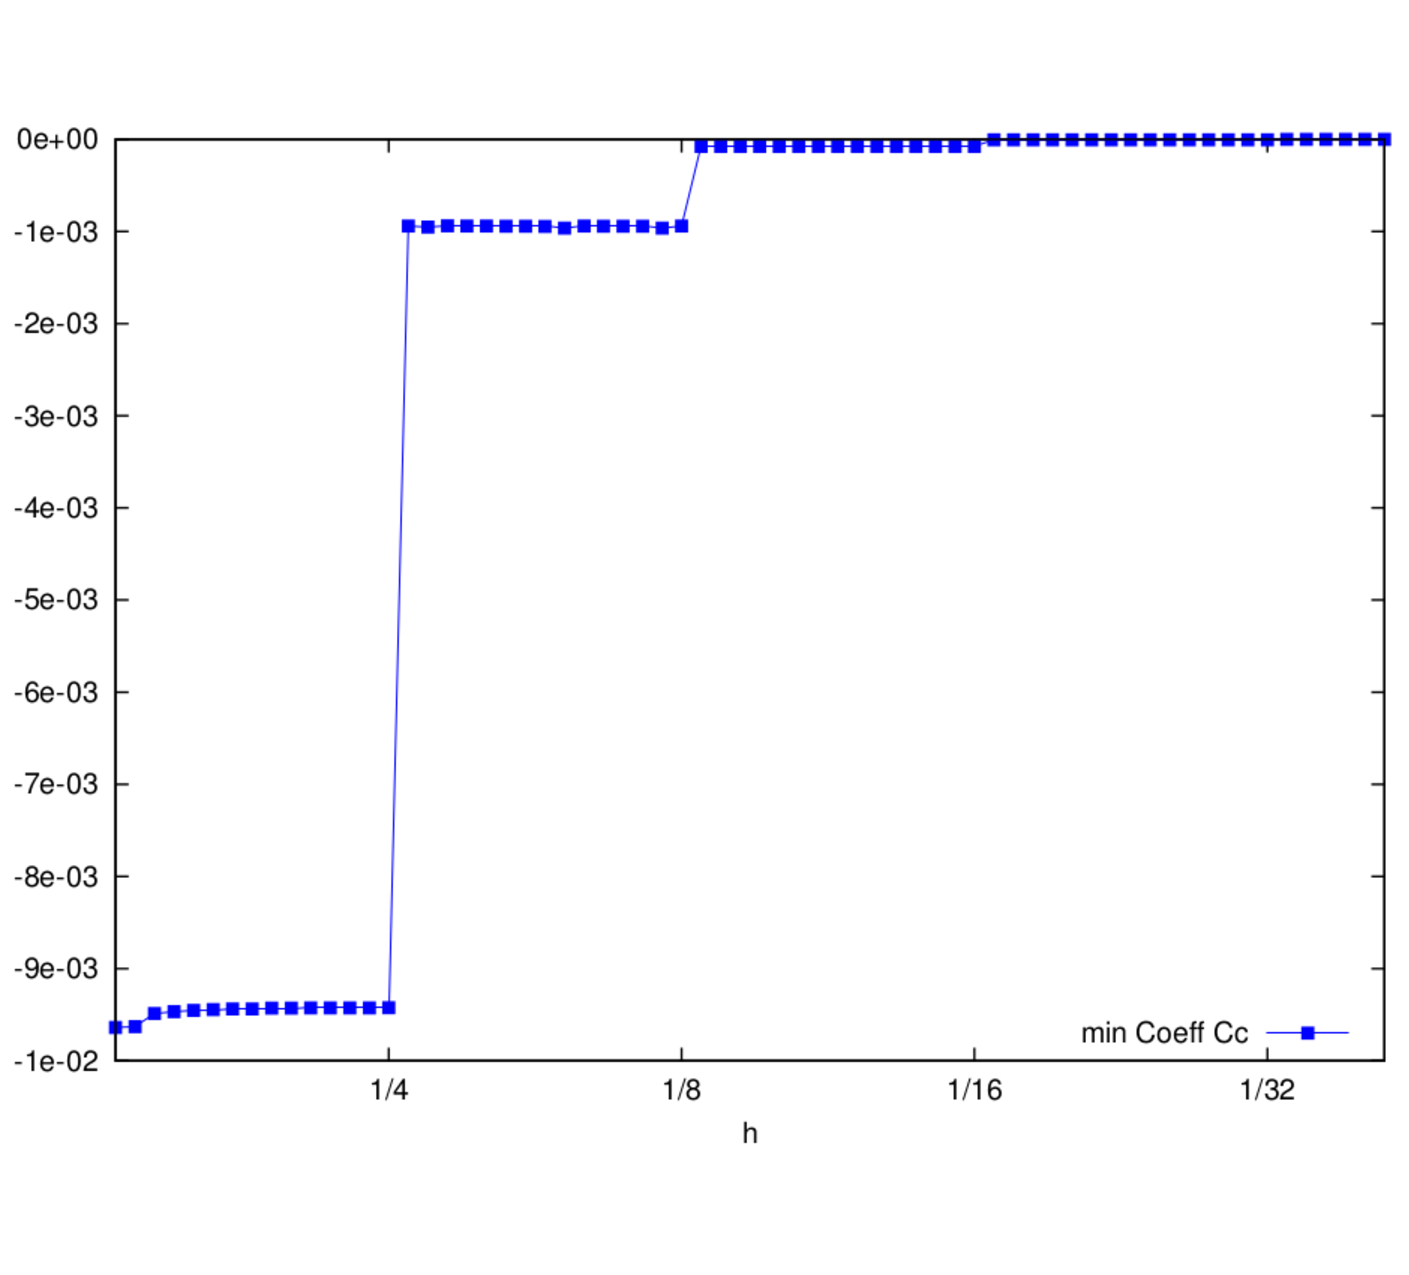
\includegraphics[scale=0.25]{plots/MA1_minCoeff.pdf}
		\caption{Minimal entry in the vector $C c$}
		\label{fig: convex min coeffs}
	\end{subfigure}	
	\caption{$L^2$ errors for test case \ref{test smooth} and additional convexification}
	\label{fig: Compare test smooth ourMethodConvex}
\end{figure}


The other test cases produce similar results such that we can assume the presented convexification is not sensible in the context of the Picard iteration.

%\begin{figure}[H]
%\centering
%	\includegraphics[scale =0.4]{plots/MA2_convexify.pdf}
%	\caption{$L^2$ errors for test case \ref{test singularity} and additional convexification}
%	\label{fig: l2 errors test singularity ourMethodConvex}
%\end{figure}
%\begin{figure}[H]
%\centering
%	\includegraphics[scale =0.4]{plots/MA2_convexComp.pdf}
%	\caption{$L^2$ errors for test case \ref{test singularity} and additional convexification}
%	\label{fig: Compare test singularity ourMethodConvex}
%\end{figure}


	

\subsection{Results without Convexification}

We use the same code basis as in the previous tests but turn off every direct convexification. Additionally the basis polynomials are chosen to be the Lagrange basis polynomials. Beside that the settings are not altered, i.e. the parameter were taken to be $\sigma = 20 k^2$, $\sigma_G$=50, $\alpha=0.3$ and $\varepsilon = 1e-2$. 
In Figure \ref{fig: l2 errors test smooth ourMethod} and Table \ref{tab: l2 errors our method} can see the results for the the smooth test case \ref{test smooth}: Again in the plot every point represents the $L^2$ error after a Picard step, whereas the table shows the error value after 15 iterations on the same grid.
\begin{figure}[H]
	\centering
	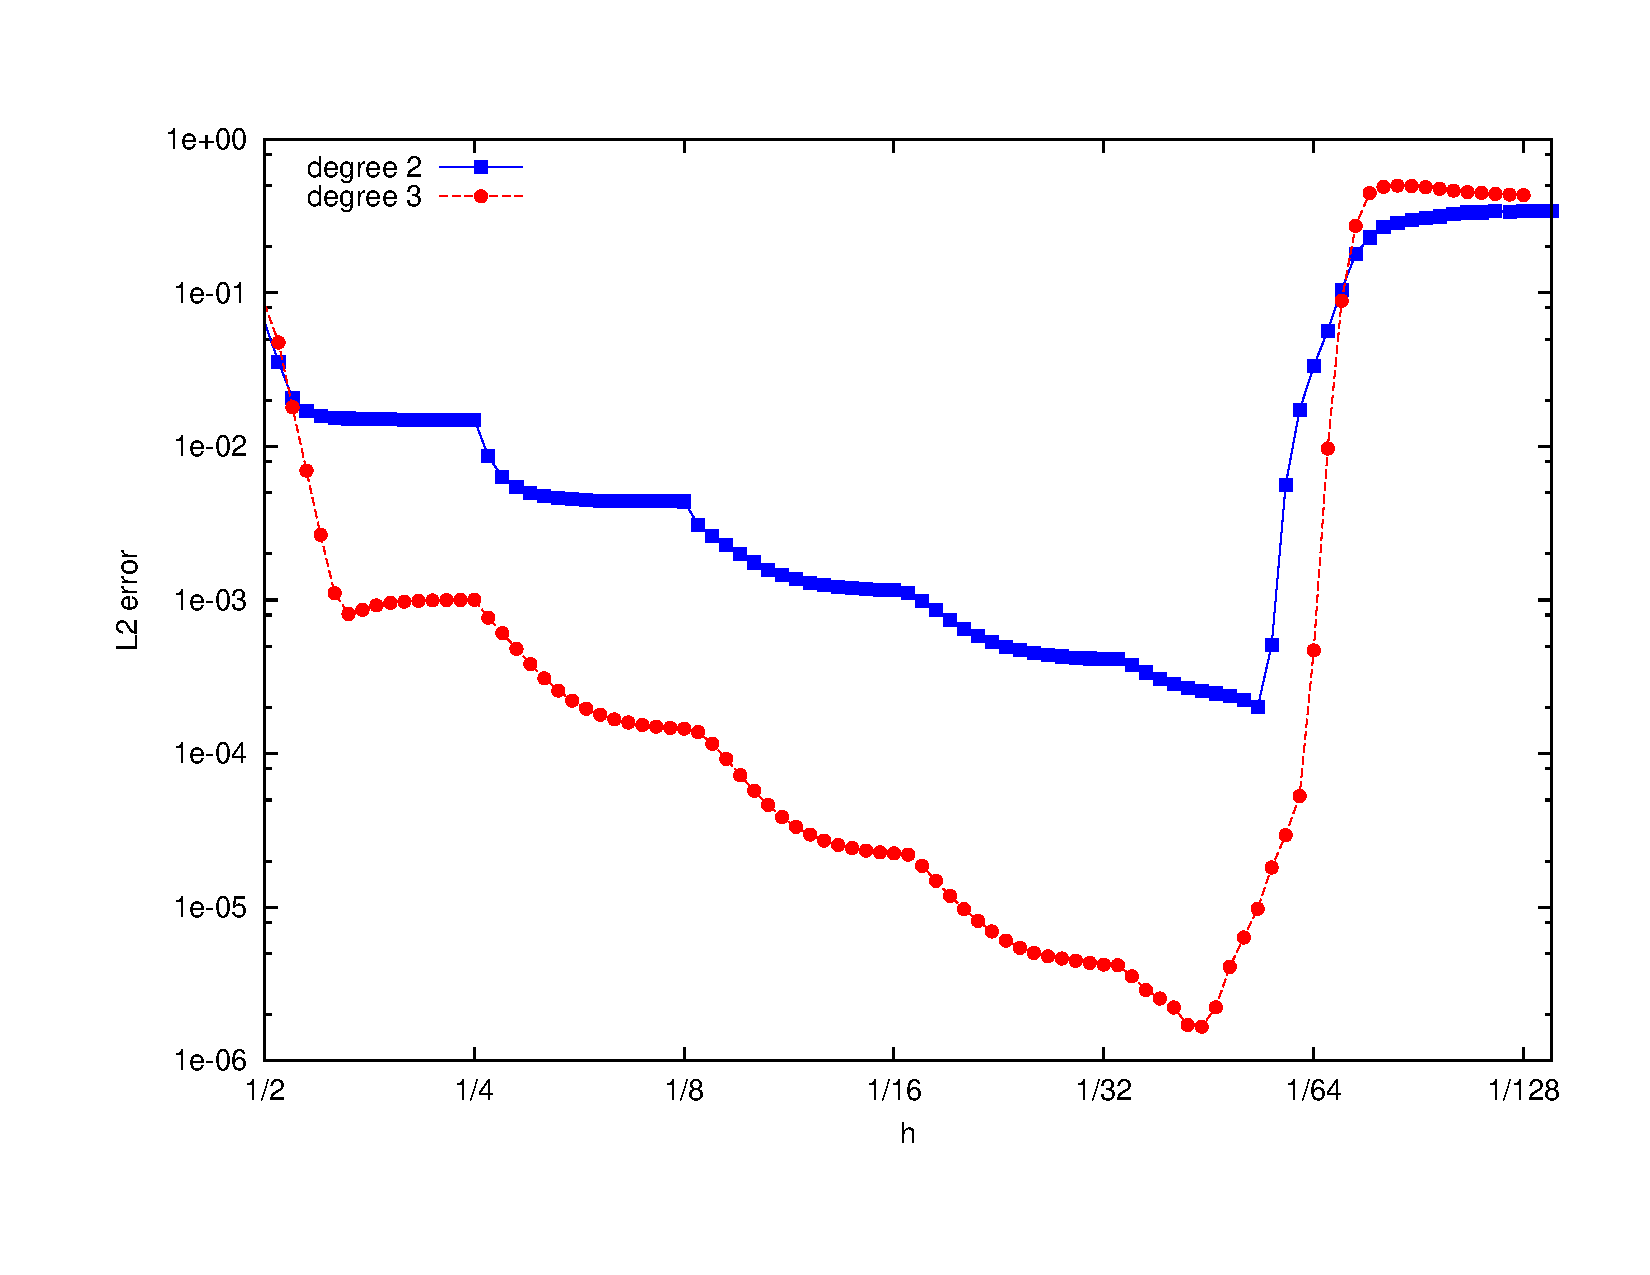
\includegraphics[scale =0.4]{plots/MA1.pdf}
	\caption{$L^2$ errors for test case \ref{test smooth}}
	\label{fig: l2 errors test smooth ourMethod}
\end{figure}
\begin{table}[H]
	\centering
	\begin{subtable}[b]{0.45\textwidth}
		\centering
		\pgfplotstabletypeset[
			every row 0 column 0/.style={set content=init},
		]
		{
		iterations  l2error
		0 0.116217
		1 0.0149796
		2 0.00439385
		3 0.00116137
		4 0.000413233
		5 0.0332876
		6 0.341691
		}
		\caption{$L^2$ error for $k=2$}
	\end{subtable}
	\begin{subtable}[b]{0.45\textwidth}
		\centering
		\pgfplotstabletypeset[
			every row 0 column 0/.style={set content=init},
		]
		{
			iterations  l2error
			0 0.151798
			1 0.00100398
			2 0.000145466
			3 2.2412e-05
			4 4.23972e-06
			5 0.000469984
			6 0.433164
				
		}
		\caption{$L^2$ error for $k=3$}
	\end{subtable}
	\caption{$L^2$ errors for test \ref{test smooth}}
	\label{tab: l2 errors our method}
\end{table}
 For the first four refinements the method behaves well for both $k=2$ and $k=3$. Afterwards the numerical solution departs from the actual solution.
 
 To exclude a break down of the linear solver, I verified that the condition of the system matrices is handled by Eigen's cholesky solver.

%To decrease the influence of the penalty paramter $\sigma$ for quadratic polynomials strong boundary conditions were introduced, i.e. instead of forcing the boundary conditions weakly by the penalty term 
%\[
%	\sum_{e \in \edgesb} \frac \sigma {|e|} \myIntS {e} { v g}
%\]
%all coefficients of base polynomials, which have support at the boundary, were fixed such that they satisfy the boundary condition given by $g$ at a set of equidistant boundary points. 
Since the influence of the gradient penalty term (cf. Section \ref{subsec: add penalty param}) on the solution is not clear, Figure \ref{fig: sigma variation} and Table \ref{tab: sigma variation} show runs with different choices of $\sigma^G$, where $\alpha$ is still fixed to $\alpha=0.3$.
\begin{figure}[H]
	\centering
	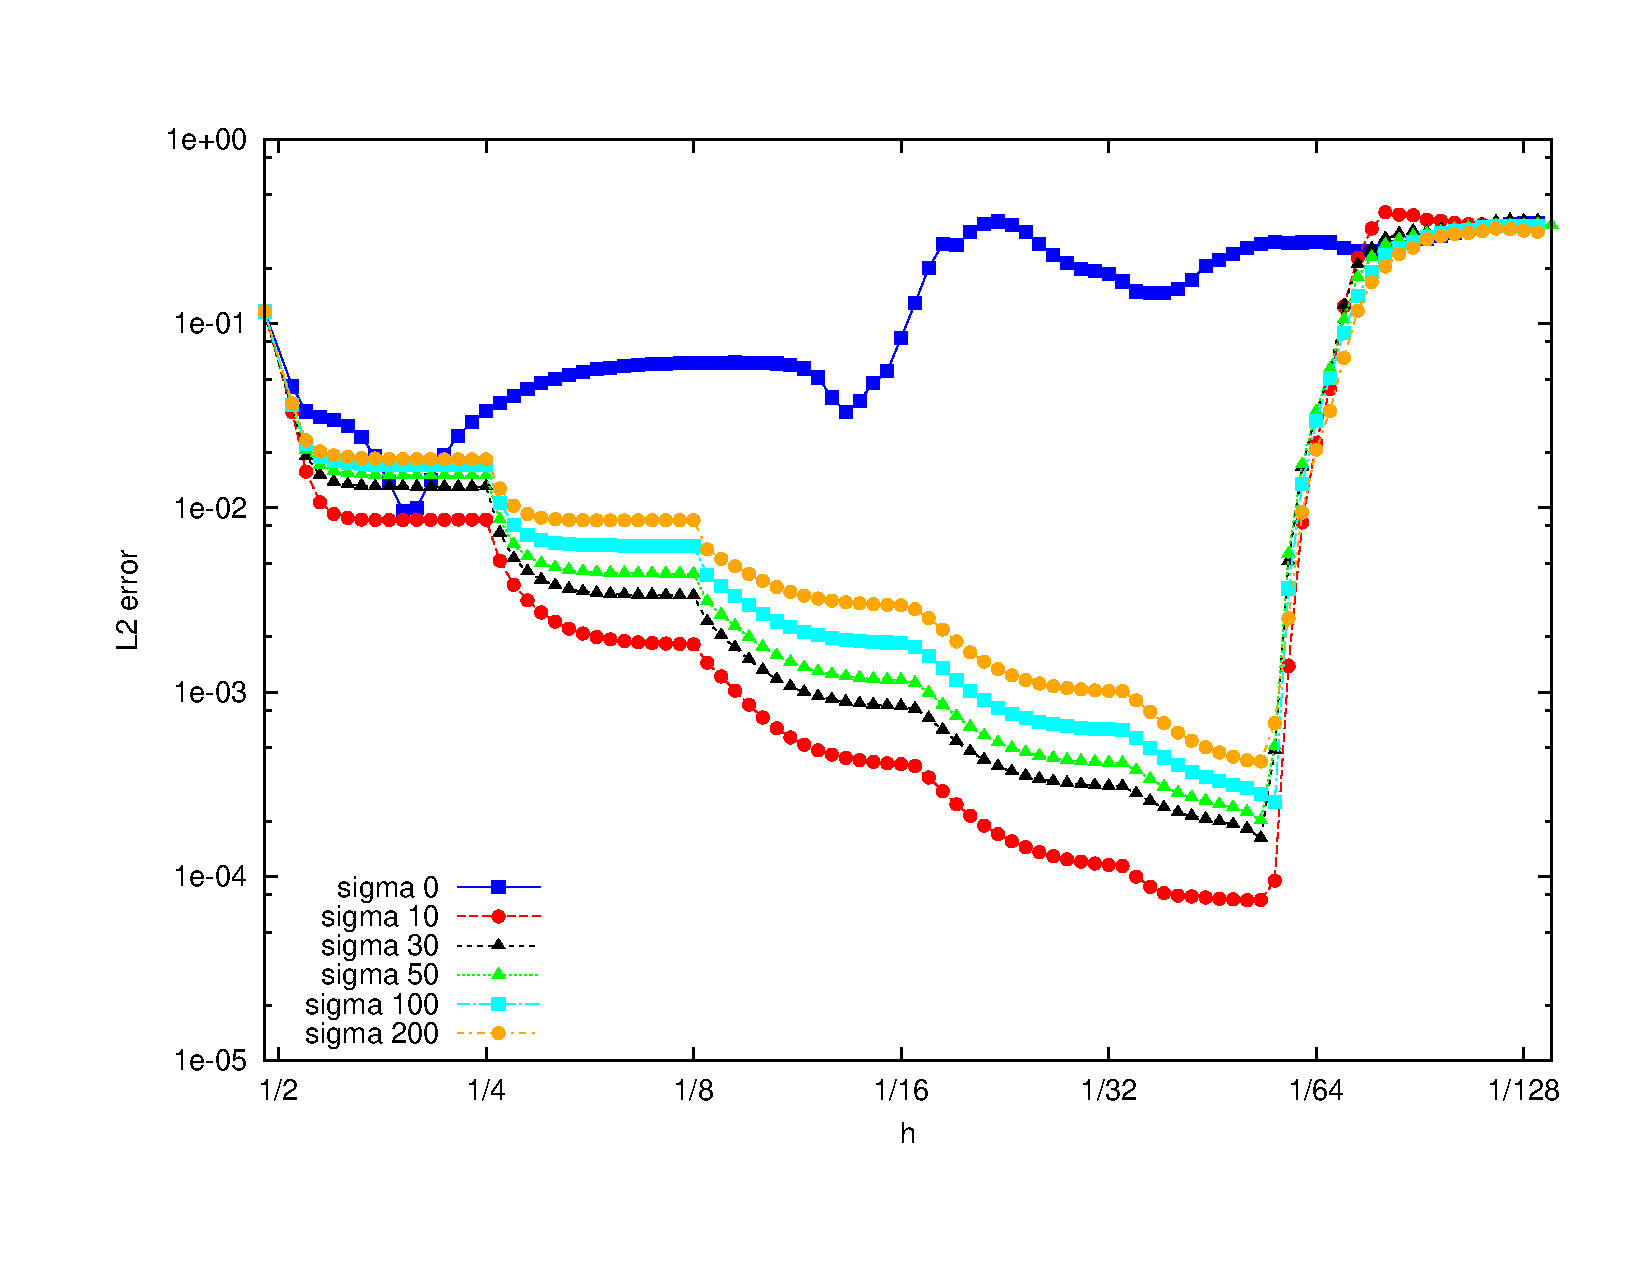
\includegraphics[scale =0.4]{plots/MA1_deg2_sigma.pdf}
	\caption{$L^2$ errors for different choices of $\sigma^G$}
	\label{fig: sigma variation}
\end{figure}

\pgfkeys{
	/pgfplots/table/string type in dec sep align/.style={
		string type,
		postproc cell content/.code={%
			\ifnum\pgfplotstablepartno=0%
			\pgfkeys{/pgfplots/table/@cell content/.add={}{&}}
			\fi
		}%
	}
}

\begin{table}[H]
	\centering
	\pgfplotstabletypeset[
	columns={iterations, 10, 30,50,10,100,200},
%	columns/0/.style={column name=$h$},
	columns/10/.style={column name={$\sigma^G$=10 }, dec sep align},
	columns/30/.style={column name={$\sigma^G=$30 }, dec sep align},
	columns/50/.style={column name={$\sigma^G=50$ }, dec sep align},
	columns/70/.style={column name={$\sigma^G=70$ }, dec sep align},
	columns/100/.style={column name={$\sigma^G=100$ }, dec sep align},
	columns/200/.style={column name={$\sigma^G=200$ }, dec sep align},
	every first column/.style={/pgf/number format/precision=0},
	%		every/.style={
	/pgf/number format/sci e, 
	/pgf/number format/fixed zerofill=true,  % print trailing zeros
	/pgf/number format/sci precision=4,     % print 14 digits
	/pgf/number format/precision=4     % print 14 digits
		%	}
	]{
		iterations 10 30 50 70 100 200
		1 0.0086428 0.0130318 0.0149796 0.016074 0.0170381 0.0183565
		2 0.00182679 0.00334291 0.00439385 0.00522693 0.00624324 0.00857697
		3 0.000407317 0.000845756 0.00116137 0.0014516 0.00184986 0.00297013
		4 0.000115474 0.000309124 0.000413233 0.00050331 0.000628928 0.00101445
		5 0.0226132 0.0328956 0.0332876 0.0322666 0.0297026 0.0207637
		6 0.331674 0.360471 0.341691 0.360872 0.338608 0.326064
	}
	\caption{$L^2$ errors for different choices of $\sigma^G$}
	\label{tab: sigma variation}
\end{table}

As we already experienced in Section \ref{subsec: add penalty param} switching the gradient penalty off, i.e. $\sigma^G=0$, proves useless. However, decreasing the penalty parameter yields better approximation results, yet varying $\sigma^G$ does not change the instability of the method.

Further, to test the choice of the parameter $\alpha$ test case \ref{test smooth} was carried out for different choices of $\alpha$, the penalty parameter $\sigma^G$ was taken to be 10. The results can be found in Figure \ref{fig: alpha variation} and Table \ref{tab: alpha variation}. %, Figure \ref{fig: alpha close up} shows a Close up of the first iterations.
 
\begin{figure}[H]
\centering
	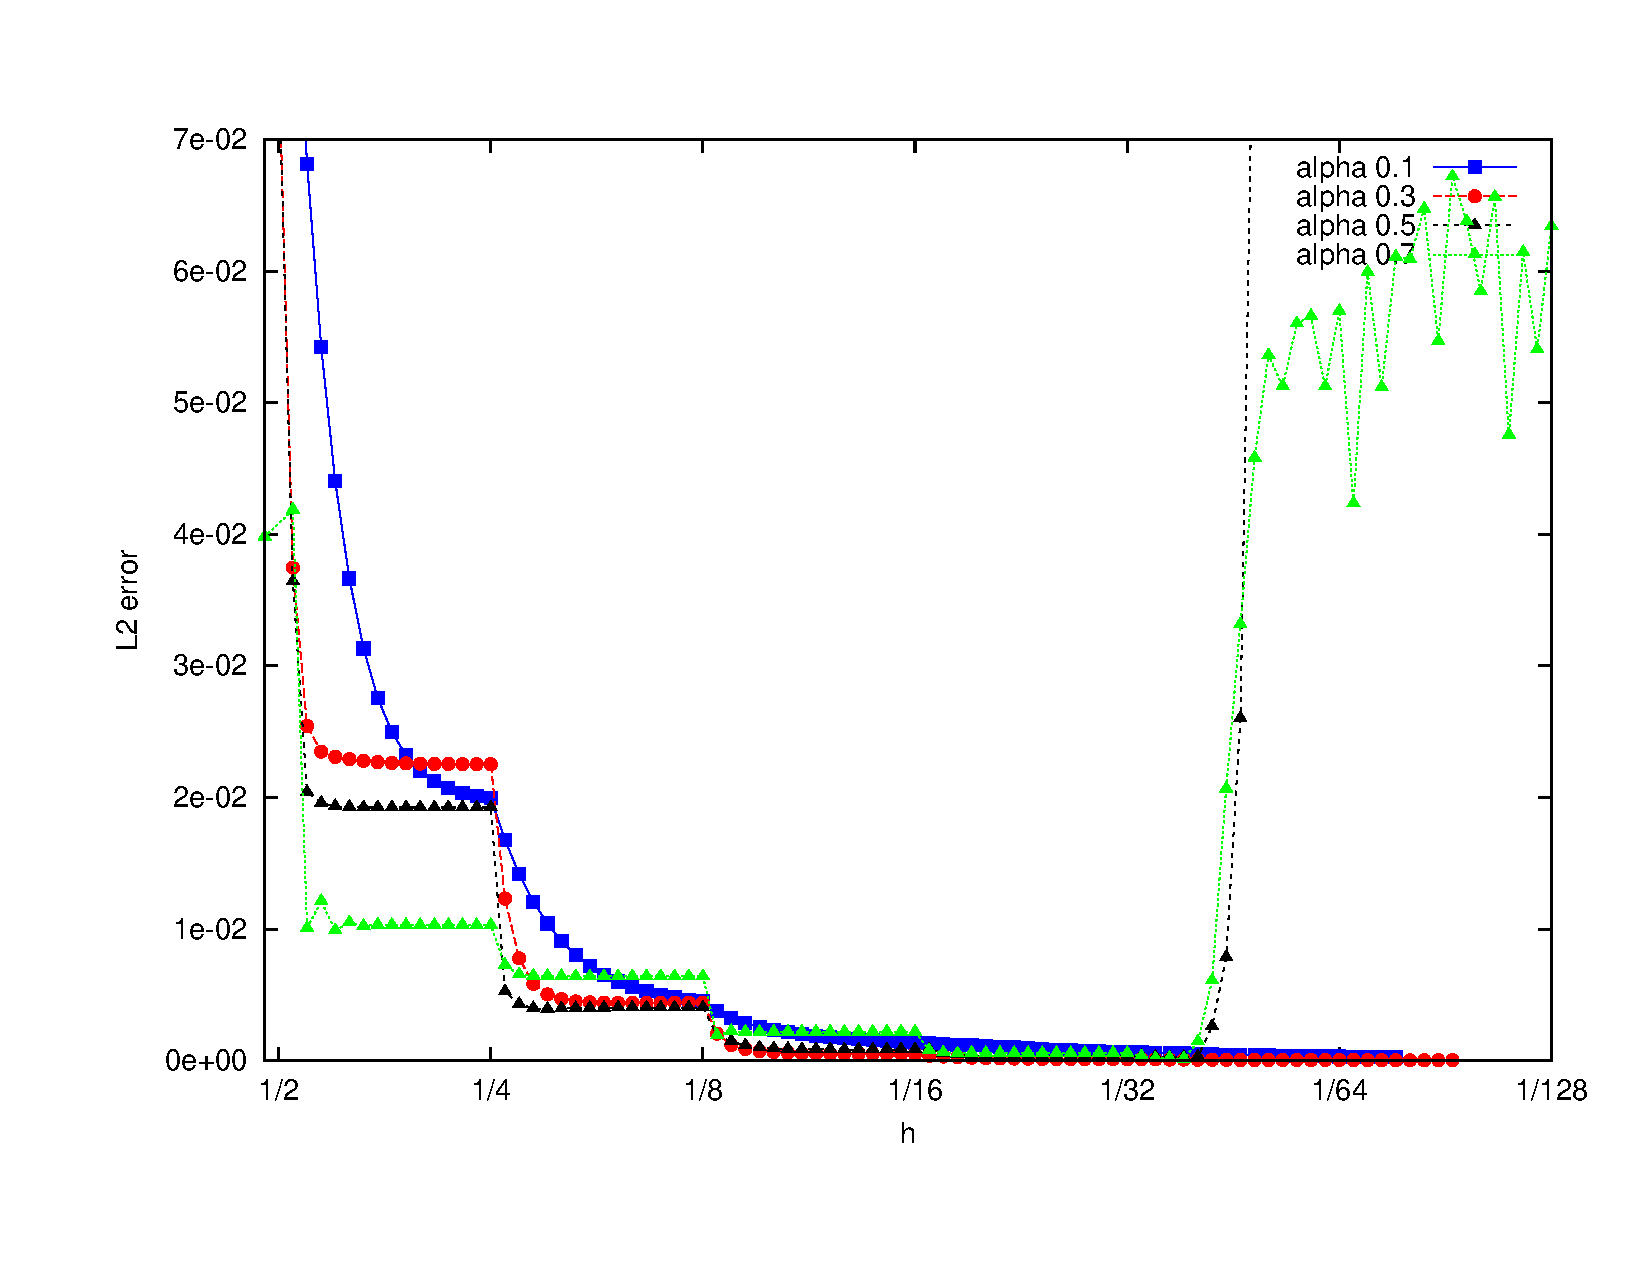
\includegraphics[scale =0.4]{plots/MA1_deg2_alpha.pdf}
	\caption{$L^2$ errors for different choices of $\alpha$}
	\label{fig: alpha variation}
\end{figure}
%
%\begin{figure}[H]
%\centering
%	\includegraphics[scale =0.35]{plots/MA1_deg2_alphaCloseUp.pdf}
%	\caption{$L^2$ errors for different choices of $\alpha$}
%	\label{fig: alpha close up}
%\end{figure}

\begin{table}[H]
	\centering
	\pgfplotstabletypeset[
		columns/0/.style={column name=$h$},
		columns/1/.style={column name={$\alpha$=0.1 }, dec sep align,      % align on the decimal marker
			},
		columns/2/.style={column name={$\alpha=0.3$ }, dec sep align},
		columns/3/.style={column name={$\alpha=0.5$ }, dec sep align},
		columns/4/.style={column name={$\alpha=0.7$ }, dec sep align},
		every first column/.style={string type},
%		every/.style={
		/pgf/number format/sci e, 
%		/pgf/number format/fixed zerofill=true,  % print trailing zeros
		/pgf/number format/sci precision=4 ,    % print 14 digits
		/pgf/number format/precision=4     % print 14 digits
		%	}
	]{
		{$h$} 1 2 3 4
		{1/2} 0.00999324  0.00864529 0.00864962 0.00864956
		{1/4} 0.00260673 0.00182038 0.00180498 0.00180486
		{1/8} 0.000986361 0.000407317 0.000395512 0.000395319
		{1/16} 0.000363884 0.000115474 0.000154169 0.213579
		{1/32} 0.000144468 0.0226132 0.30321 0.331661
		{1/64} 0.000967598 0.331674 0.361392 0.320555

	}
	\caption{$L^2$ errors for different choices of $\alpha$}
	\label{tab: alpha variation}
\end{table}

As to expect a larger choice of $\alpha$ leads to a faster decrease of the error, on the coarsest grids all solutions Picard iterations converge to approximations with the same error norm. One can verify that those approximations are numerically equal. We observe that for $\alpha=0.1$ the choice of 15 iterations is too small as we obtain a larger $L^2$ error than with the other values.\\
But as in the previous setting at same point all methods become instable and diverge. Though we note that choosing a smaller $\alpha$ slows down this process. 

  \begin{figure}[H]
  	\centering
  	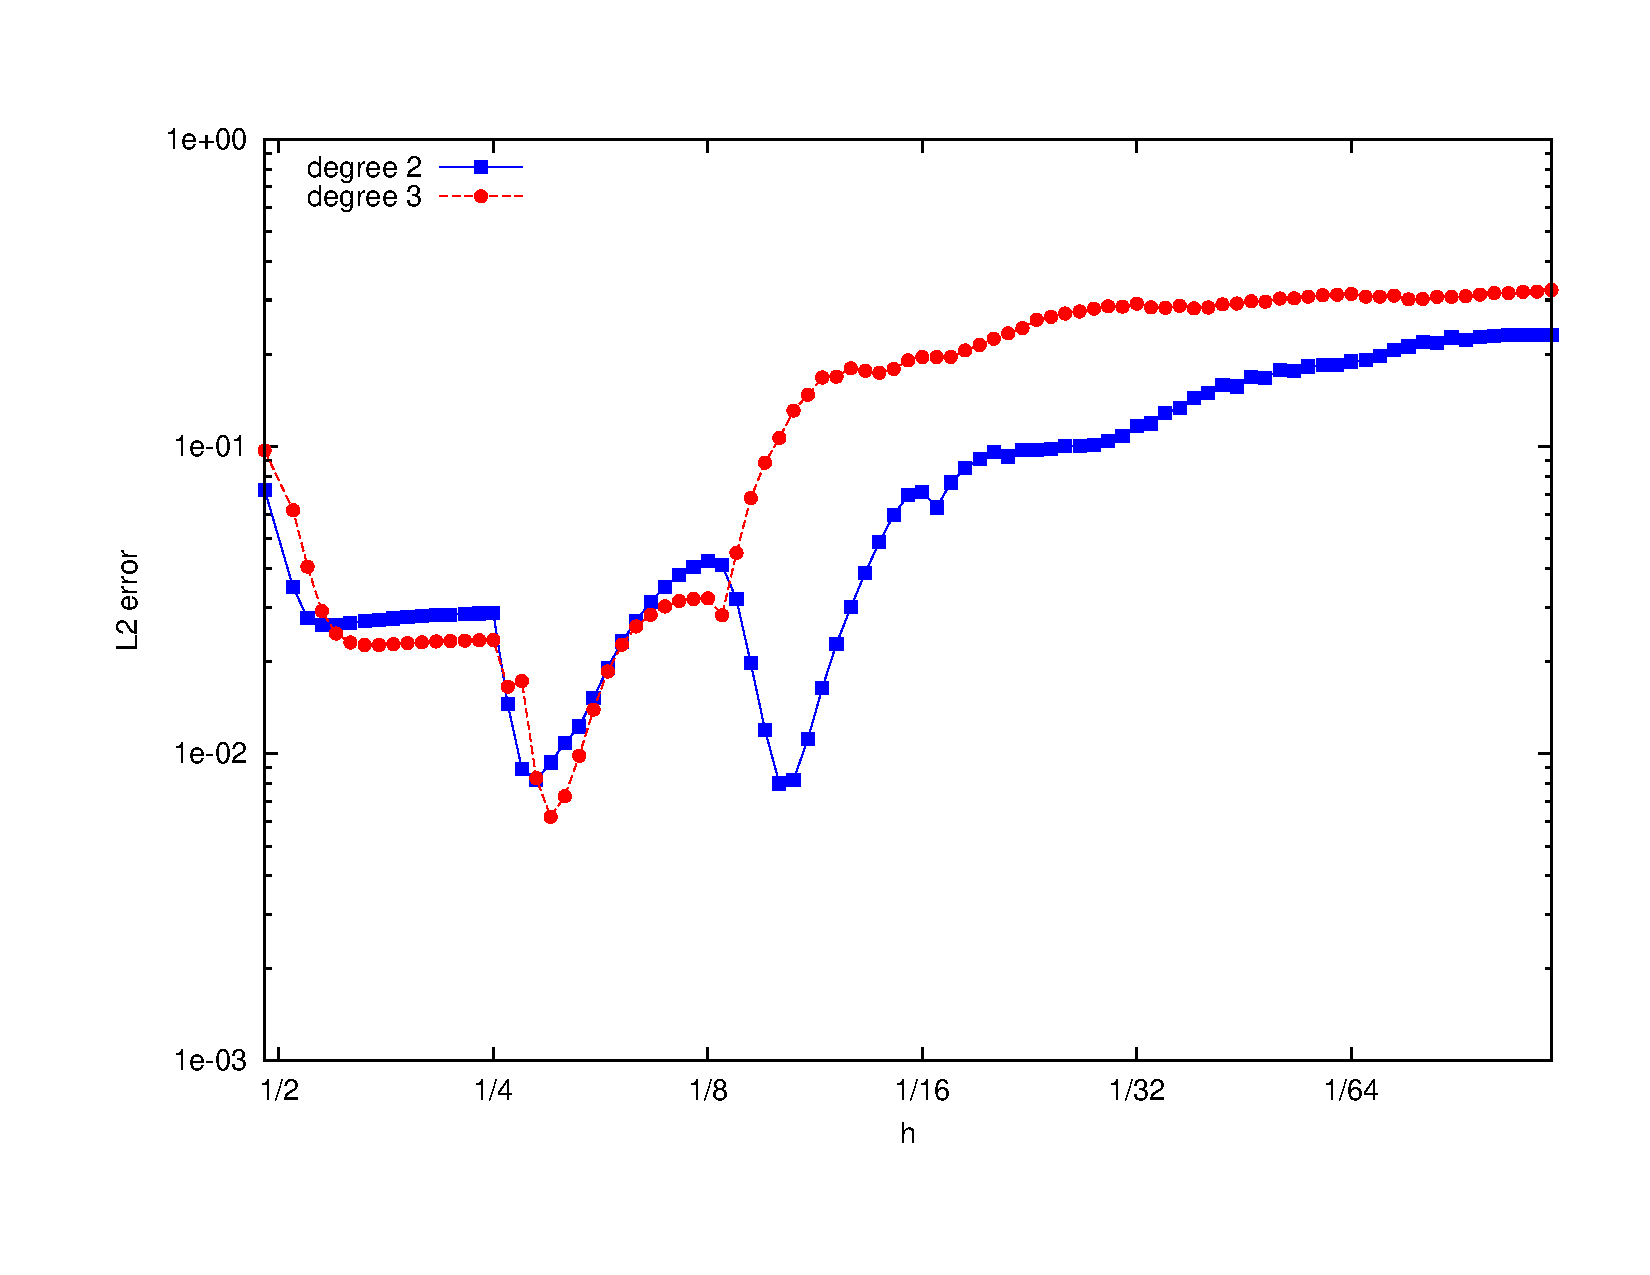
\includegraphics[scale =0.37]{plots/MA3.pdf}
  	\caption{$L^2$ errors for test case \ref{test sqrt}}
  	\label{fig: l2 errors test sqrt ourMethod}
  \end{figure}
  
  
  \begin{figure}[H]
  	\centering
  	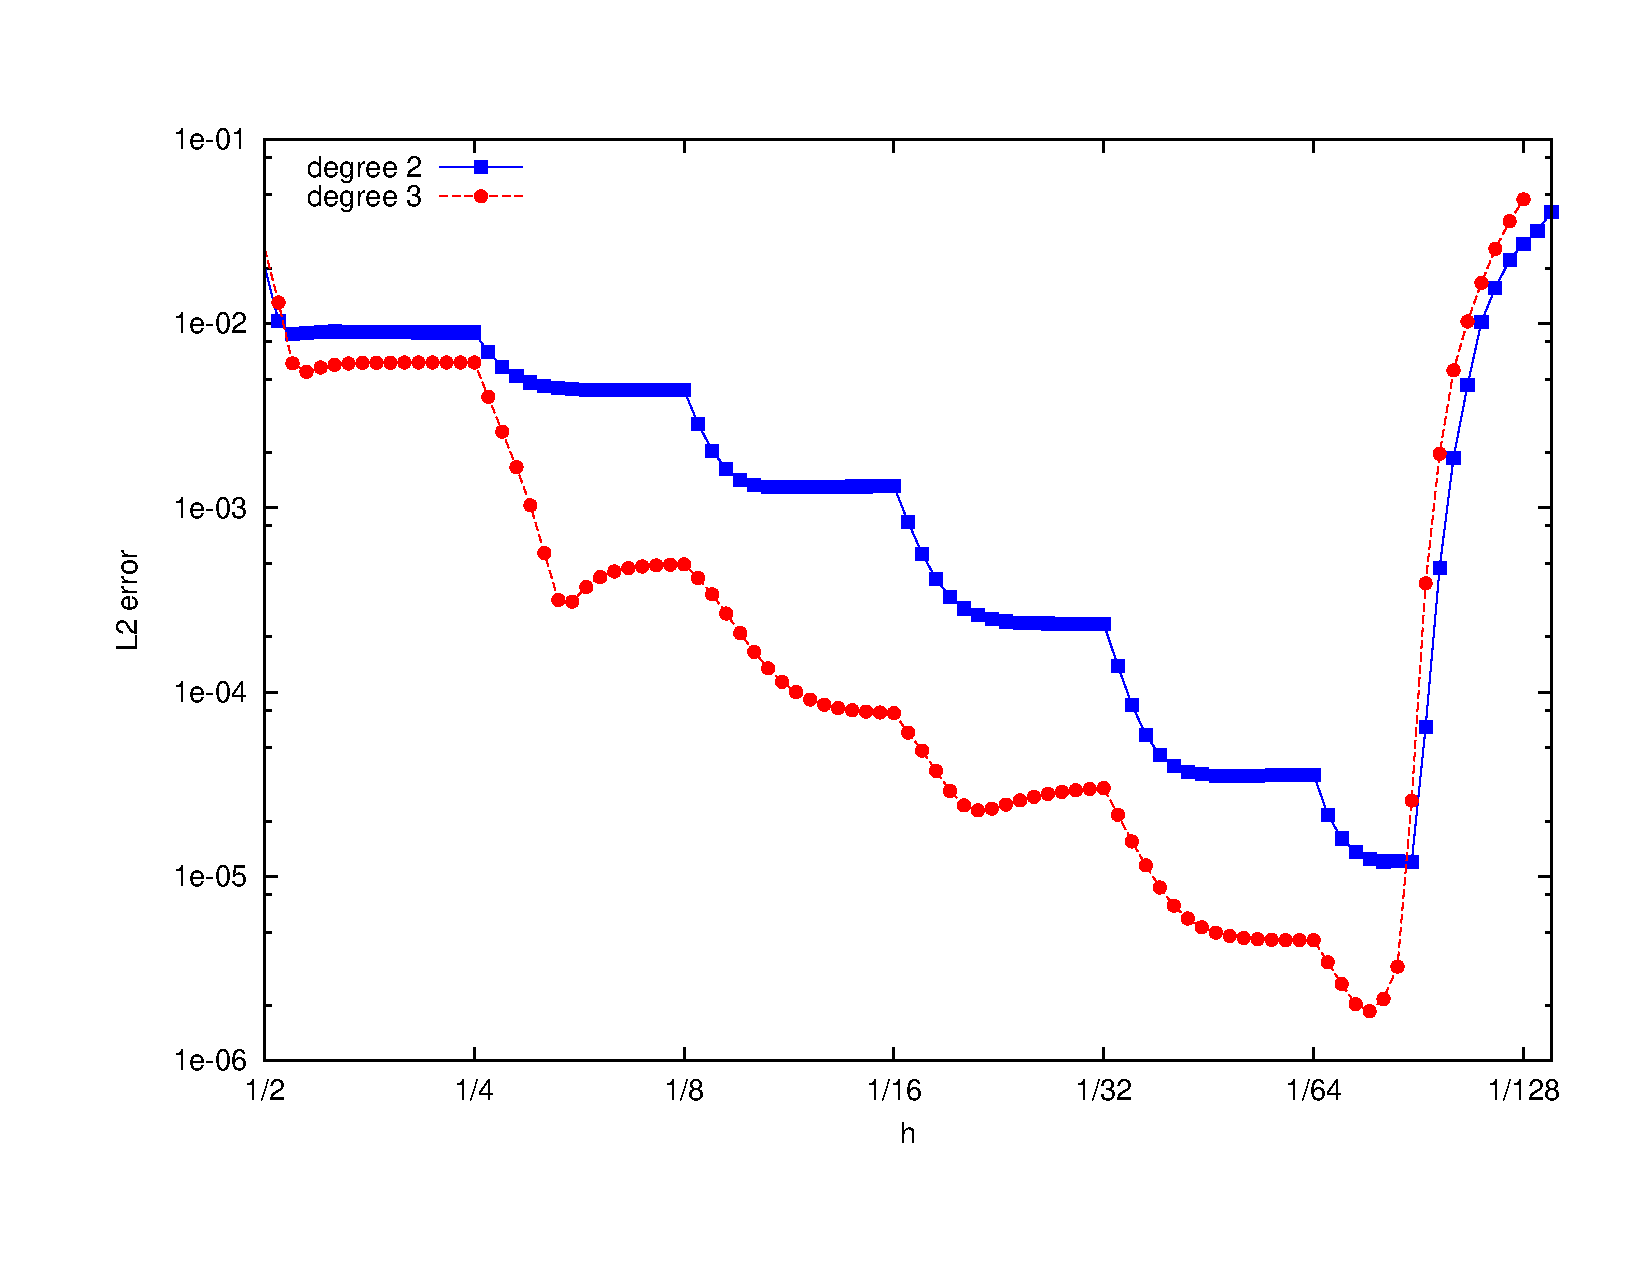
\includegraphics[scale =0.37]{plots/MA2.pdf}
  	\caption{$L^2$ errors for test case \ref{test singularity}}
  	\label{fig: l2 errors test singularity ourMethod}
  \end{figure}
We get similiar results in the next two cases albeit the fixed point iterations performs worse in the second case which lacks $H^2$ regularity. The $L^2$ errors are shown in the Figures \ref{fig: l2 errors test sqrt ourMethod} and \ref{fig: l2 errors test singularity ourMethod}, $\alpha$ was taken to be 0.3 and $\sigma^G$ to be 10. In the last example \ref{test dirac} the Picard iteration showed no signs of convergence at all.

  

The results were validated by a reference implementation using the finite element tool FEniCS. Albeit I was not able to include the modified cofactor matrix to the bilinear form the error behaved as in the computational results of the C++ code. It decreased for the first four refinements and diverged afterwards. 

Additionally one can in the FEniCS variant the cofactor matrix of the Hessian which is evaluated piecewise replace by the discrete Hessian as defined in \ref{def: discrete Hessian} for a symmetric ansatz space $\Sigma_h$. The code can be found in the Appendix \ref{app: our code}. Also experiments with this symmetric discrete Hessian ended in an unstable method.

\chapter{Conclusion und Perspective}
\label{ch:conclusion}
\section{Comparison with Newton's method}

Before we start the anlaysis of our Method we shortly see what happens if we apply Newton's method on the analytical form of the \MA equation \ref{MA eq}.
Let $F$ be the function such that its root solves the \MA equation, i.e. 
\[
	F(u) = \mydet{D^2 u} -f
\]
Applying Newton's method on $F(u) =0$ we have
\begin{align}
	DF[u^n](u^{i+1}-u^i) = -F[u^i]
\end{align}
where $DF[u]$ denotes the G\^ateaux derivative. We derived the G\^ateaux derivative $DF[u] v = \mycof{D^2 u}:D^2v$ already in theorem \ref{thm: linearisation} leading us to the Newton iteration
\begin{align}
	\mycof{D^2 u^i}:D^2\left(u^{i+1}-u^i\right) &= -\mydet{D^2 u^i}+f \nonumber \\
	\Leftrightarrow \qquad \qquad  \mycof{D^2 u^i}:D^2(u^{i+1}) &= -\mydet{D^2 u^i} +f  +\mycof{D^2 u^i}:D^2(u^i). \label{eq: Newton iteration pre}
\end{align}

Similar to the derivation of the fixed point iteration we can apply Lemma \ref{la: An application of the divergernce product rule} to rewrite \eqref{eq: Newton iteration pre} and we have the problem
\begin{align}
	\nabla \cdot \left( \cof(D^2 u^0) \nabla u^{i+1} \right) &= -\mydet {D^2u^i} +f+\nabla \cdot \left( \cof(D^2 u^i) \nabla u^{i} \right)  \textnormal{ in } \Omega,  \label{eq: Newton iteration}\\
	u^{i+1} &= g \textnormal{ on } \partial \Omega .
\end{align}

Hence, considering once again the fact 
\[
\nabla \cdot \left( \mycof {D^2 u } \nabla v \right)
\stackrel{La.\ref{la: An application of the divergernce product rule}}=\nabla \cdot {}\mycof{D^2 u}:D^2u
=\frac 1 2 \mydet{D^2u}.
\]
we can see our method as a variant of Newton's method. 

In \cite{Awanou2014} Awanou analysed the similar iteration process
\begin{align}
	\nabla \cdot \left( \cof(D^2 u^0) \nabla u^{i+1} \right) &= \nabla \cdot \left( \cof(D^2 u^0) \nabla u^{i} \right) + f - \operatorname{det} (D^2u^i) \textnormal{ in } \Omega,  \label{eq: Awanout eq}\\
	u^{i+1} &= g \textnormal{ on } \partial \Omega.
\end{align}
showing convergence for the analytical solution $u$ and a sufficent close $u^0$. 
In a earlier work \cite{Awanou2010} Awanou examined a discrete Version of a vanishing moment method, herein he mentioned a method he calls Newton's method defined by
\[
	\int_{\Omega} [\mycof{ D^2 u_h^i} Du_h^{i+1}] \cdot Dv_h = -	\int_{\Omega} f v_h + \frac 1 2 \int_{\Omega} [\mycof{ D^2 u_h^i} Du_h^{i}] \cdot Dv_h \; \forall v_h \in V_h \cap H^1_0 (\Omega)  \label{eq: Awanout eq2}.
\]
And indeed this is the variational form of \eqref{eq: Newton iteration}
His chosen trial space were piecewise polynomials contained in $C^1(\Omega)$. He claims that this ansatz breaks down for problems with non-smooth solutions, in his numerical results he cites test \ref{test sqrt} as an example where Newton's method diverges.

\todo{existence theory}
\section{Comparison with the $C^0$ penalty method}
It is also interesting to compare our linearisation with the linearisations of the two other methods.
Consider a Newton step made in the $C^0$ penalty method (cf. \ref{sec: Brenner method}).
\begin{align}
	&\int_\Omega \cofHess {u^i} \nabla (u^{i+1}-u^i) \nabla v - \sum_{e \in \edgesb} \int_e \cofHess {u^i} \nabla (u^{i+1}-u^i) \cdot \mathbf n \; v \nonumber \\
	&- \sum_{e \in \edgesb} \int_e \cofHess {u^i} \nabla v \cdot \mathbf n (u^{i+1}-u^i) + \sigma \sum_{e \in \edgesb} \frac 1 {|e|} \int_e v (u^{i+1}-u^i)\nonumber \\
	=&-\int_\Omega \left(f - \detHess{u^i)}\right) v  
			- \sum_{e \in \edgesi} \int_e \jump { \average{\cofHess {u^i}} \nabla {u^i} } v \nonumber \\
&	- \sum_{e \in \edgesb} \int_e \cofHess {u^i} \nabla v \cdot \mathbf n \; (u^i-g) - \sigma \sum_{e \in \edgesb} \frac 1 {|e|} \int_e v (u^{i}-g) \label{eq: a newton step Brenner}
\end{align}
To compare both linearisations we first reorder and remove cancelling terms in \eqref{eq: a newton step Brenner}.
\begin{align}
	&\int_\Omega \cofHess {u^i} \nabla u^{i+1} \nabla v \\
	&- \sum_{e \in \edgesb} \int_e \cofHess {u^i} \nabla u^{i+1} \cdot \mathbf n \; v 
		- \sum_{e \in \edgesb} \int_e \cofHess {u^i} \nabla v \cdot \mathbf n \; u^{i+1} \\
	&+\sigma \sum_{e \in \edgesb} \frac 1 {|e|} \int_e v u^{i+1}\\
	=
	&-\int_\Omega \left(f - \detHess{u^i)}\right) v \\
	&- \sum_{e \in \edgesi} \int_e \jump { \average{\cofHess {u^i}} \nabla {u^i} } v 
		+ \sum_{e \in \edgesb} \int_e \cofHess {u^i} \nabla {u^i} \cdot \mathbf n \; v\\
	&- 2\sum_{e \in \edgesb} \int_e \cofHess {u^i} \nabla v \cdot \mathbf n \; {u^i}
		+ \sum_{e \in \edgesb} \int_e \cofHess {u^i} \nabla v \cdot \mathbf n \; g \\
	&+\sigma \sum_{e \in \edgesb} \frac 1 {|e|} \int_e v g \label{eq: ordered newton step Brenner}
\end{align}

\section{Conclusion}

We saw the performances of three DG methods solving PDEs of \MA type.
The first method, introduced by Brenner et alter yields a good result for the smooth test case but failed for every other test case, even for test case \ref{test singularity} that has a solution in $C^1(\Omega)$. Hence, as the developer indicate in their paper it is only suitable for finding classical solutions.
Brenner et alter used a vanishing moment method to find a proper initial guess. This seems rather costly and our numerical results show the method could be improved using a nested iterations and a simple linear PDE for the first initial guess.

The results Neilan showed in his paper for our second examined method look very promising.
Note, that this method has if polynomial degree of $V_h$ and $\Sigma_h$ are chosen equally has as five times as many degree of freedoms compared to both other methods.

The last presented method turned out to be a variant of an classical damped Newton approach. 
\todo{verbesserung mit modifizierter cofactor matrix}
The classical approach is known to fail for elements which are not at least contained in $C^1(\Omega)$. Unfortunately the fixed point iteration do also diverge for finer grids. Yet it may serve for an initial guess during a multilevel method. For big grid widths in our test cases the $L2$ error even decreased for problems which do not have a classical solution.

Comparing the three methods for the smooth test case the first and second method produce similar convergence orders while the first has less degree of freedoms. The Picard type method yields even for the first four refinement a much smaller convergence rate.

We saw that recent DG methods perform well on problems with classical solution, but have problems with problems with only viscocity solution or Aleksandrov solutions. Most rely on Newton's method to solve their nonlinear system and how to provide good initial guesses is not answered yet.
My numerical results show that a nested iteration approach often does not provide suitable starting points for further refinements.

\section{Perspective}
Handling fully nonlinear PDEs is a complex domain and results on this domain are very unsatisfactory when compared to the linear case. Even when restrict ourselves to the prototype of nonlinear PDEs, the \MA equation, the theory is far from being complete for both the analytical and the numerical point of view.

Recent DG methods work provably well for classical solutions, but to the author's knowledge there are no proven statement on their performance for viscosity solutions or Aleksandrov solutions. Even in the case we have a classical solution convergence of DG method is only proven for polynomial degrees greater or equal than three. Though most numerical experiment suggest a relaxation it could not be proved yet.

We presented methods for the \MA equation given that the right-hand side only depend on $x$ and the left-hand side only on the determinant of the Hessian. Currently DG methods were often not extended to more general PDEs. It has to be analysed, if  discretisations for right-hand sides depending on $u$ and $\nabla u$ and more complicated left-hand sides may be derived analogously. An example for one of those more complicated left-hand sides is $\mydet {D^2 u +A}$ for $A:\Omega \rightarrow \R^{d \times d}$.
 
The implemented convexification did not support the solution process. Yet, it is worth to address this approach further. Maybe it is useful to convexify intermediate solution only on fine grids.




%\chapter*{Acknowledgements}

\begin{appendices}

%\section{FEniCS Code for General Setting}
\lstinputlisting{Source_Code/MA_problem.py}

\section{FEniCS Code for C0 penalty Method (cf. Section \ref{sec: Brenner method})} \label{app: Code Brenner}
\lstinputlisting{../../FEniCS/source/DG_Brenner.py}
\section{FEniCS Code for Discrete Hessian Method (cf. \ref{sec: FEM discrete Hessian})} \label{app: Code Neilan}
\lstinputlisting{Source_Code/DG_neilan.py}

\section{FEniCS Code for Picard Iteration (cf. Chapter \ref{ch:ourMethod})} \label{app: our code}
\lstinputlisting{Source_Code/MA_iterated_withNeilan.py}
	
\end{appendices}



\newpage
%\input{literatur.tex}
% bib
\newpage
%\nocite*{} 
\bibliography{literatur.bib,my_additional_bibliography.bib}
\bibliographystyle{plain}
\end{document}
